\documentclass[12pt]{report}

%======================
% Packages
%======================
\usepackage[a4paper,margin=1in]{geometry}
\usepackage{placeins}
\usepackage{setspace}
\usepackage{titlesec}
\usepackage{graphicx}
\usepackage{amsmath}
\usepackage{float}
\usepackage{xcolor}
\usepackage{draftfigure}
\usepackage[utf8]{inputenc}
\usepackage{textcomp}
\usepackage{textgreek}
\usepackage{xcolor}
\usepackage{caption}
\usepackage{caption}
\usepackage{setspace}
\usepackage{graphicx}
\usepackage{subcaption}
\usepackage{colortbl}
\usepackage{array}
\usepackage[table]{xcolor}

% Global caption style
\captionsetup{
	font=small,              % slightly smaller than body text
	labelfont=bf,            % Figure 1 in bold
	textfont=it,             % caption text in italic (Nature-like)
	labelsep=period,        % "Figure 1. Caption text"
	justification=justified,
	singlelinecheck=false,
	skip=6pt                % space between figure and caption
}
% Hyperref (MUST be last)
\usepackage[hidelinks]{hyperref}

\hypersetup{
	colorlinks=true,
	linkcolor=blue,
	citecolor=teal,
	urlcolor=violet
}

\onehalfspacing

%\flushbottom

%======================
\begin{document}
	
	%======================
	% Title Page
	%======================
	\begin{titlepage}
		\centering
		
		%======================
		% University Logo
		%======================
		
\includegraphics[width=0.2\textwidth]{logo}\\[1cm]
		
		%======================
		% University Name
		%======================
		{\Large Ferdowsi University of Mashhad}\\
		{\large Faculty of Engineering}\\[1.5cm]
		
		%======================
		% Title
		%======================
		{\Large \textbf{MSc Dissertation}}\\[1cm]
		
		{\large \textbf{Investigation of the correlation between the spatial distribution of sleep spindles and the relationship between the thalamocortical and hippocampal networks in mice}}\\[2cm]
		
		%======================
		% Author
		%======================
		\textbf{By:}\\
		Daniel Dehghan Ortekand\\[1cm]
		
		%======================
		% Supervisor
		%======================
		\textbf{Supervisor:}\\
		Dr. Maryam Ghorbani\\[2cm]
		
		%======================
		% Date
		%======================
		February 2024
		
	\end{titlepage}
	
	%======================
	% Abstract
	%======================
	\chapter*{Abstract}
	\addcontentsline{toc}{chapter}{Abstract}
	\setlength{\parindent}{0pt}
	
	Neural information exchange occurs both spatially and temporally. Moreover, the coupling between sleep spindles and slow oscillations reflects inter-network communications and the memory consolidation process. In recent years, various studies have been conducted on data recorded from the brains of humans and different animals to examine the spatial distribution of brain oscillations, including characteristic sleep oscillations such as spindle propagation and slow waves. These studies directly and indirectly indicate that the distribution and propagation of brain oscillations significantly affect neuronal activity and the rate of information transfer between different brain regions. Other studies suggest that the propagation of brain waves can directly influence memory recall and retention.\\[0.01cm]
	
	Additionally, certain sleep oscillations, when coupled with other oscillations, can specifically cause a significant increase in neuronal activity during that time frame.\\[0.01cm]
	
	In this study, conducted on mouse LFP data, we initially separated sleep spindles and then categorized slow oscillations into local and global, as well as single-peaked and double-peaked groups. Our findings demonstrate a significant correlation between neuronal activity and sleep events such as sleep spindles and slow oscillations. On the other hand, propagation in the thalamus was examined in all sessions, and characteristics such as period and amplitude for these events were compared with each other. Subsequently, to better understand the relationship between these two events, their Phase-Amplitude Coupling (PAC) was examined, and their phases showed significant differences.\\ [0.01cm]
	
	Finally, to investigate the relationship between the hippocampus and thalamus regions, PAC analysis was performed between global and local sleep spindles and ripples, and a significant correlation was observed for the phase.\\[0.01cm]
	
	\textbf{Keywords}: Sleep wave propagation, LFP, Sleep spindles, Slow oscillations, Sleep
	\newpage
	
	%======================
	% Lists
	%======================
	\pagenumbering{roman}
	
	\setcounter{tocdepth}{3}
	\tableofcontents
	\newpage
	
	\listoffigures
	\newpage
	
	%======================
	% Main Content
	%======================
	\pagenumbering{arabic}
	
	%======================
	\chapter{Introduction}
	\label{Introduction}
	At the beginning of this chapter, the different stages of sleep are first described. Subsequently, the key characteristics of NREM\footnote{None rapid eye movement} sleep, including sleep spindles, slow oscillations (SOs), and sharp-wave ripples (SPW-Rs), are introduced. Finally, the recording of local field potentials (LFPs) and electroencephalography (EEG) is discussed.
	
	\section{Sleep Stages}
	\label{sec:sleep-stages}
	
	Sleep is one of the most important aspects of the life of living organisms. Recent studies have shown that the transition from short-term to long-term memory occurs during NREM sleep\cite{Ghorbani2020}. This process consists of the following three stages:
	In humans, sleep is divided into two major states:
	\begin{itemize}
		\item Encoding
		\item Consolidation
		\item Retrieval
	\end{itemize}
	On the other hand, studies have shown that sleep consists of different stages across various animal species. For example, human sleep is broadly divided into two main categories: rapid eye movement (REM) sleep and non-rapid eye movement (NREM) sleep. One of the main characteristics of REM\footnote{Rapid eye movement} sleep is the low amplitude and high frequency of the recorded EEG signals\cite{Marshall2020}\cite{Watson2016}. Dreaming also occurs primarily during REM sleep\cite{Bandarabadi2020}.
	
	NREM sleep, in contrast, consists of three distinct stages, which are described below.
	
	\subsection{Stage 1 (NREM1)}
	\label{sec:Stage_1_(NREM1)}
	The first stage of NREM sleep is the lightest stage of sleep. During this stage, an individual gradually transitions into sleep. Examination of the EEG recordings under these conditions typically reveals alpha and theta oscillations\cite{Ghorbani2020}. The main characteristics of alpha and theta oscillations include their frequency ranges, which are approximately 8–10 Hz\footnote{Hertz} and 4–8 Hz, respectively. In addition, a reduction in activity can be observed in both the electrooculography (EOG) and electromyography (EMG) recordings during this stage of sleep.
	
	
	\subsection{Stage 2 (NREM2)}
	\label{sec:Stage_2_(NREM2)}
	In this stage of NREM sleep, characteristic oscillatory patterns known as K-complexes can be observed (Figure~\ref{fig:Sleep spindle and K-complex in the EEG signal}). Other oscillatory patterns, known as sleep spindles, can also be detected during this stage. These oscillations typically occur over a short period of time and within two distinct frequency ranges in the cortical and thalamic regions of the brain (Figure~\ref{fig:Sleep spindle and K-complex in the EEG signal})\cite{Sato2022}. Thalamocortical sleep spindles can be broadly classified into slow spindles (6–12 Hz) and fast spindles (13–17 Hz), which exhibit distinct characteristics\cite{Hashemi2019}.
	
	\begin{figure}[H]
		\centering
		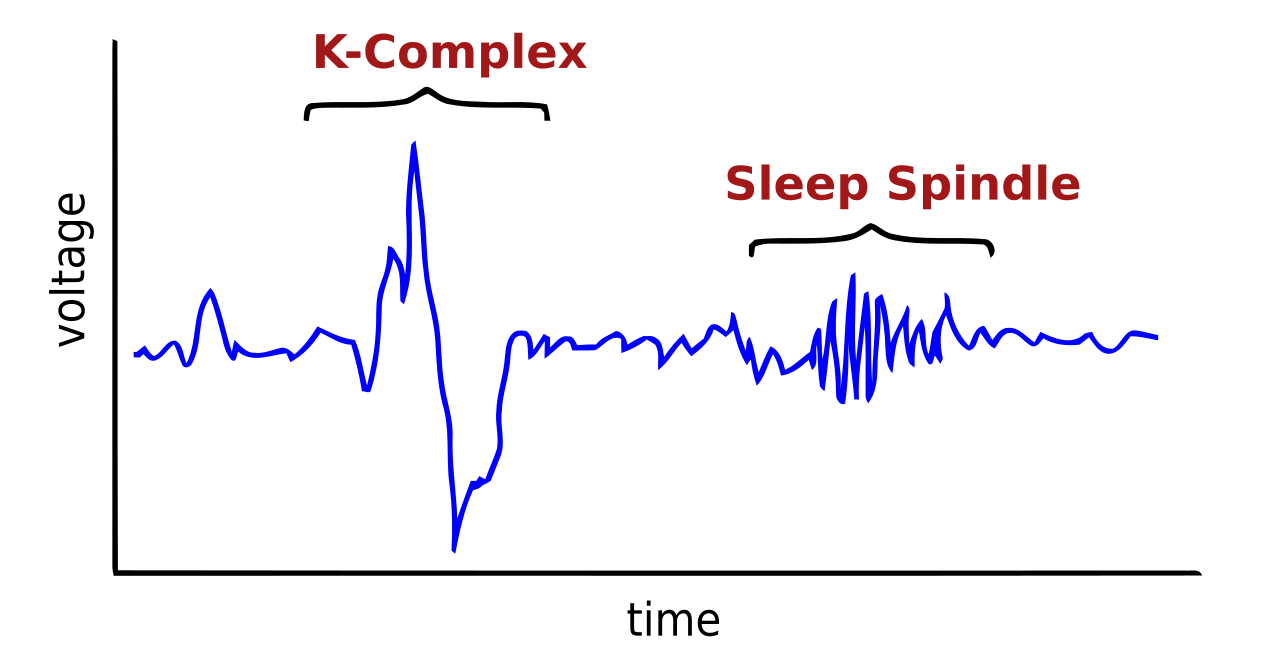
\includegraphics[width=0.8\linewidth]{fig1.1.png}
		\caption{Sleep spindle and K-complex in the EEG signal\cite{Cay2022}}
		\label{fig:Sleep spindle and K-complex in the EEG signal}
	\end{figure}
	
	\subsection{Stage 3 (NREM3 / Slow-Wave Sleep, SWS)}
	\label{Stage_3}
	This stage of NREM sleep occurs immediately before REM sleep or wakefulness. In fact, it represents the deepest stage of sleep and is commonly referred to as slow-wave sleep (SWS). The predominant oscillations during this stage are delta waves\cite{Ghorbani2020}(figure~\ref{Types of brain oscillations at different frequency ranges}).
	\begin{figure}[H]
		\centering
		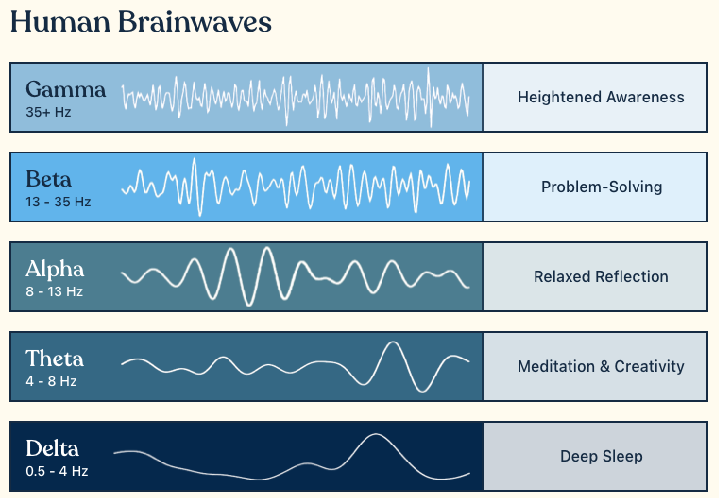
\includegraphics[width=0.8\linewidth]{fig1.2.png}
		\caption{Types of brain oscillations at different frequency ranges\cite{R2023}}
		\label{fig:Types of brain oscillations at different frequency ranges}
	\end{figure}
	Finally, it should be noted that the sleep stages in mice differ from those in humans. In mice, there is no distinct second stage of NREM sleep; instead, following the first stage, sleep progresses directly to the third stage and subsequently to either REM sleep or wakefulness\cite{Alizadeh2022}.
	
	\section{Characteristic Sleep Oscillations}
	\label{Characteristic_Sleep_Oscillations}
	As mentioned in Section~\ref{sec:sleep-stages}, sleep plays an important role in the consolidation of memories from short-term to long-term storage. However, the brain is an intrinsic oscillator\cite{Buzsaki2004}. Therefore, it is thought to support memory consolidation during sleep through its intrinsic oscillatory activity. Accordingly, it is necessary to introduce these endogenous brain oscillations.
	
	
	\subsection{Sleep spindles}
	\label{sec:Sleep spindles}
	These oscillations can be observed throughout the cortex\cite{Piantoni2017}. However, their generation originates in the thalamus. They arise from interactions between inhibitory reticular (RE) neurons and the thalamocortical network and subsequently propagate to other regions of the brain, including the cortex. The amplitude of these oscillations gradually increases from the onset of the oscillation until reaching its peak, after which it progressively decreases\cite{dehnavi2019}.
	The frequency of sleep spindles ranges from 7 to 15 Hz, with a duration of approximately 0.5 to 3 seconds. In addition, slow spindles are predominantly observed in the upper regions of the cortex, whereas fast spindles are mainly observed in the parietal region\cite{Niethard2018}\cite{Muehlroth2019}\cite{McDevitt2017}.
	
	
	\subsection{slow oscillations}
	\label{sec:slow_oscillations}
	Slow oscillations (SOs) are periodic rhythms with frequencies below 4 Hz and were first identified by Steriade and colleagues\cite{Steriade1993}. Experimental studies have shown that, during the negative slope of a slow oscillation in the local field potential (LFP) signal, cortical neurons are in a hyper-polarized state (the down state). Conversely, during the positive slope of the slow oscillation in the LFP signal, cortical neurons become depolarized and generate spikes (the up state)\cite{Contreras1995}. The neocortex is considered the primary source of SO generation, and observations indicate that cortical slow oscillatory activity is regulated by the underlying subcortical structures\cite{Timofeev2020}.
	
	Furthermore, both intracellular and extracellular recordings have shown that slow oscillations tend to propagate in either the anterior or posterior direction\cite{Luczak2007}\cite{Massimini2004}.
	
	\subsection{ripples}
	\label{sec:ripples}
	Another type of brain oscillation observed during NREM sleep is the ripple. Ripples are brief oscillations, typically lasting 50–100 ms, with a frequency range of 100–250 Hz. These oscillations occur in the hippocampus\cite{Buzski2006} and represent the most prominent self-organized event in the hippocampus. They occur when the suppression of inputs from outside the hippocampus is released\cite{Contreras1995}.
	
	In addition, sharp-wave ripples (SPW-Rs) exhibit several distinctive characteristics. First, they are among the population events of the brain. When a large number of neurons become active simultaneously, sharp-wave ripples are generated. These waves can transmit information across different regions of the brain\cite{Buzski1992}. Second, SPW-Rs are among the most highly synchronized events in the mammalian brain and are associated with transient and strong increases in excitability in the hippocampus and its associated structures\cite{Buzski2015}.
	
	\section{Electrophysiological Recordings}
	\label{sec:Electrophysiological_Recordings}
	Brain signals can generally be recorded using either invasive or non-invasive methods. In fact, the purpose of recording brain signals in humans or animals, such as mice, cats, and others, is to observe changes in the electromagnetic fields generated by the brain. In the following sections, some of these recording methods are briefly described.
	
	\subsection{Electroencephalography (EEG)}
	\label{sec:Electroencephalography _EEG)}
	Electroencephalography (EEG) is one of the oldest and most widely used methods for investigating the electrical activity of the brain\cite{Buzski2015} and is also commonly referred to as brain-wave recording (Figure~\ref{fig:fig3.1}). The EEG recorded by each scalp electrode can be considered a spatially smoothed version of the local field potential (LFP), reflecting the electrical activity generated within an area of approximately 10 cm² beneath the recording electrode\cite{Sheehy1984}.
	
	\begin{figure}[!htbp]
		\centering
		
		\begin{minipage}{0.48\textwidth}
			\centering
			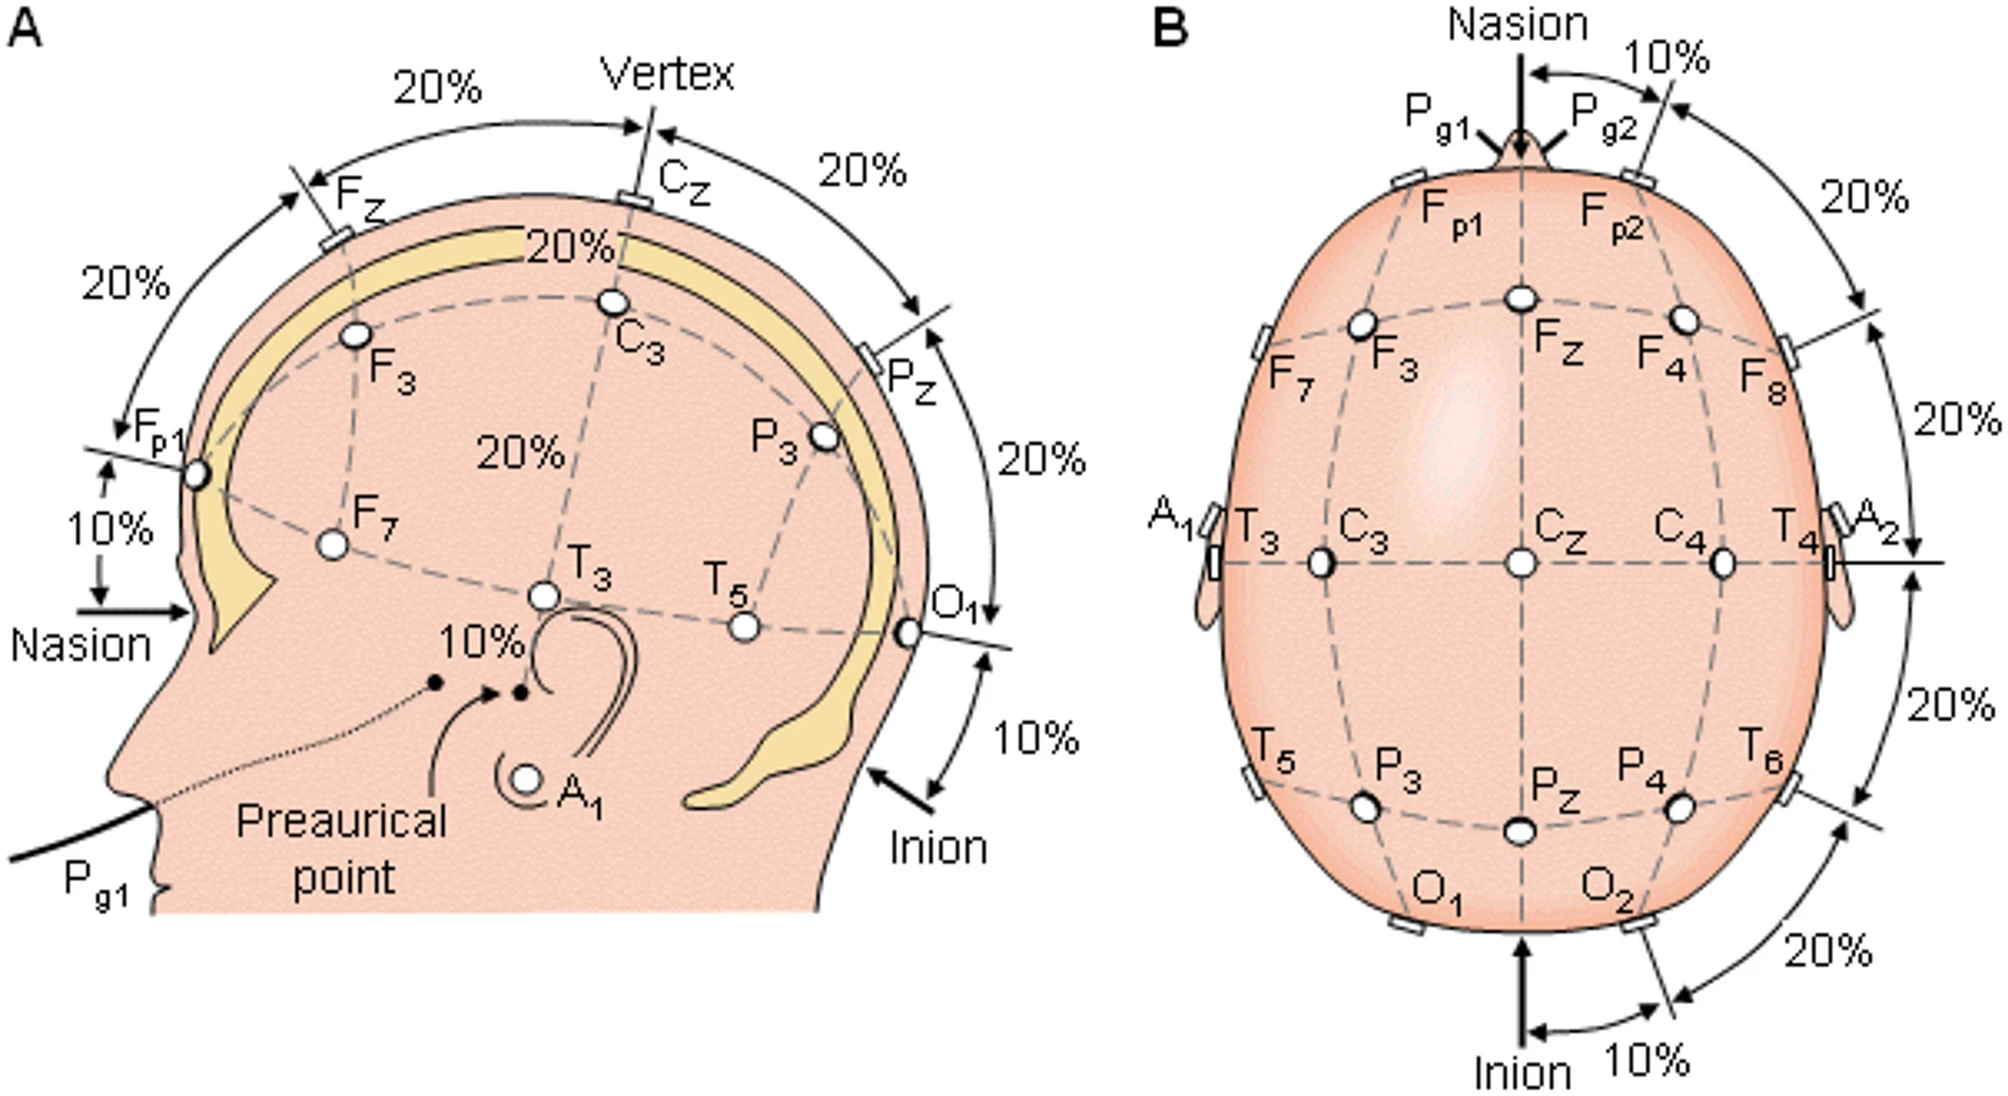
\includegraphics[width=\textwidth]{fig3.1left.png}
		\end{minipage}
		\hfill
		\begin{minipage}{0.48\textwidth}
			\centering
			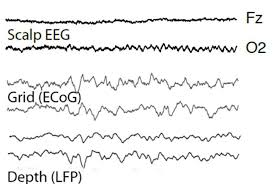
\includegraphics[width=\textwidth]{fig3.1r.jpeg}
		\end{minipage}
		
		\caption{Right: An example of EEG signals recorded from two different channels, ECOG and LFP\cite{Ghorbani2020}. Left: Electrode locations shown from the top and lateral views\cite{Xiong2025}.}
		\label{fig:fig3.1}
	\end{figure}
	
	In most cases, it is difficult to establish a reliable relationship between the EEG signal and the activity of individual neurons. This is because a combination of hard and soft tissues lies between the recording electrodes and the firing neurons. These tissues attenuate and distort the electrical signals before they reach the electrode, thereby altering the signal recorded at the electrode site\cite{Tucker1993}\cite{Ebersole1996}.
	
	\subsection{Local Field Potentials (LFPs)}
	\label{Local_Field_Potentials_(LFPs)}
	All of the signals introduced above are recorded from cortical regions, whereas local field potential (LFP) recordings capture activity from deeper brain regions, including action potentials and other oscillatory activity arising from membrane potentials at the neuronal level\cite{Buzski2015}. In addition, these recordings can be used to observe the activity of nearly all or a portion of a neuronal population within a small volume at high density\cite{Du2011}. This type of recording is referred to as multi-unit activity (MUA)\footnote{Multi unit activity} (Figure~\ref{fig:Placement of the LFP recording electrode}).
	
	\begin{figure}[H]
		\centering
		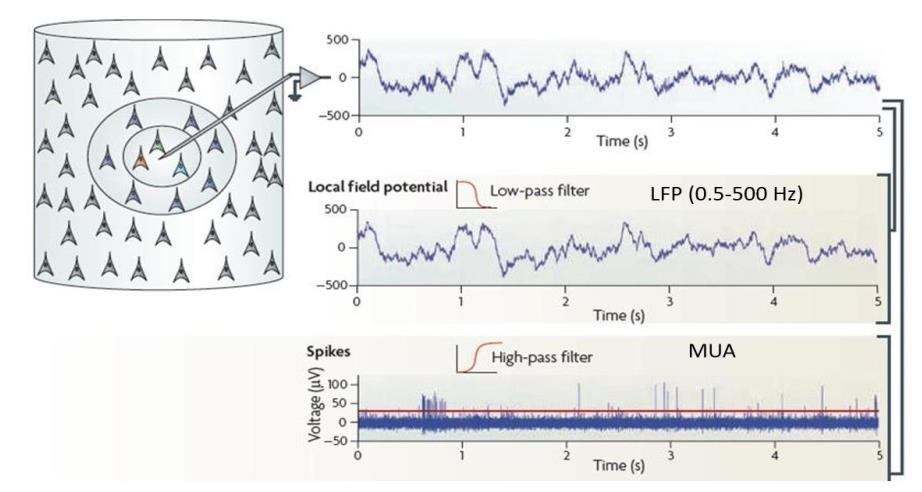
\includegraphics[width=0.8\linewidth]{fig1.4.png}
		\caption{Placement of the recording electrode, examples of the recorded signals, and extraction of LFP and MUA signals from the recordings.\cite{Ghorbani2020}}
		\label{fig:Placement of the LFP recording electrode}
	\end{figure}	
	
	\section{The Thalamus}
	\label{sec:The_Thalamus}
	Since part of the signals recorded in this study were obtained from the thalamic region of the mouse brain, a brief introduction to the thalamus is also provided.
	\subsection{Thalamus in Mice}
	\label{sec:Thalamus_in_Mice}
	The thalamus is the largest part of the diencephalon. It is located bilaterally along the dorsal aspect of the third ventricle and is bordered by the telencephalon, while its caudal portion is adjacent to the midbrain (mesencephalon). The thalamus serves as a relay station for almost all sensory inputs to the cortex, with the exception of olfactory information. The numerous thalamic nuclei can be classified into either specific nuclei, which are associated with motor, sensory, and associative functions, or nonspecific nuclei, which include the intralaminar and midline nuclei\cite{Hjornevik2007}\cite{Schrder2020}.
	In the present study, the recorded data were obtained from the anterior thalamic nucleus, which itself consists of the anterodorsal, anteromedial, and anteroventral nuclei, as shown in (Figure~\ref{fig:The thalamus in mice})\cite{Jankowski2013}.
	
	\section{The Hippocampus in Mice}
	\label{sec:The_Hippocampus}
	The hippocampus is a curved structure that extends from the septal nuclei of the ventral forebrain to the parietal cortex. It consists of the dentate gyrus (DG) and the cornu ammonis (CA) regions, including CA1–CA3. The DG is referred to as the granule cell layer because it is primarily composed of granule cells, whereas the corresponding layer in the CA regions is known as the pyramidal cell layer (Figure~\ref{fig:The hippocampus in mice})\cite{LlorensMartn2014}.
	
	\begin{figure}[H]
		\centering
		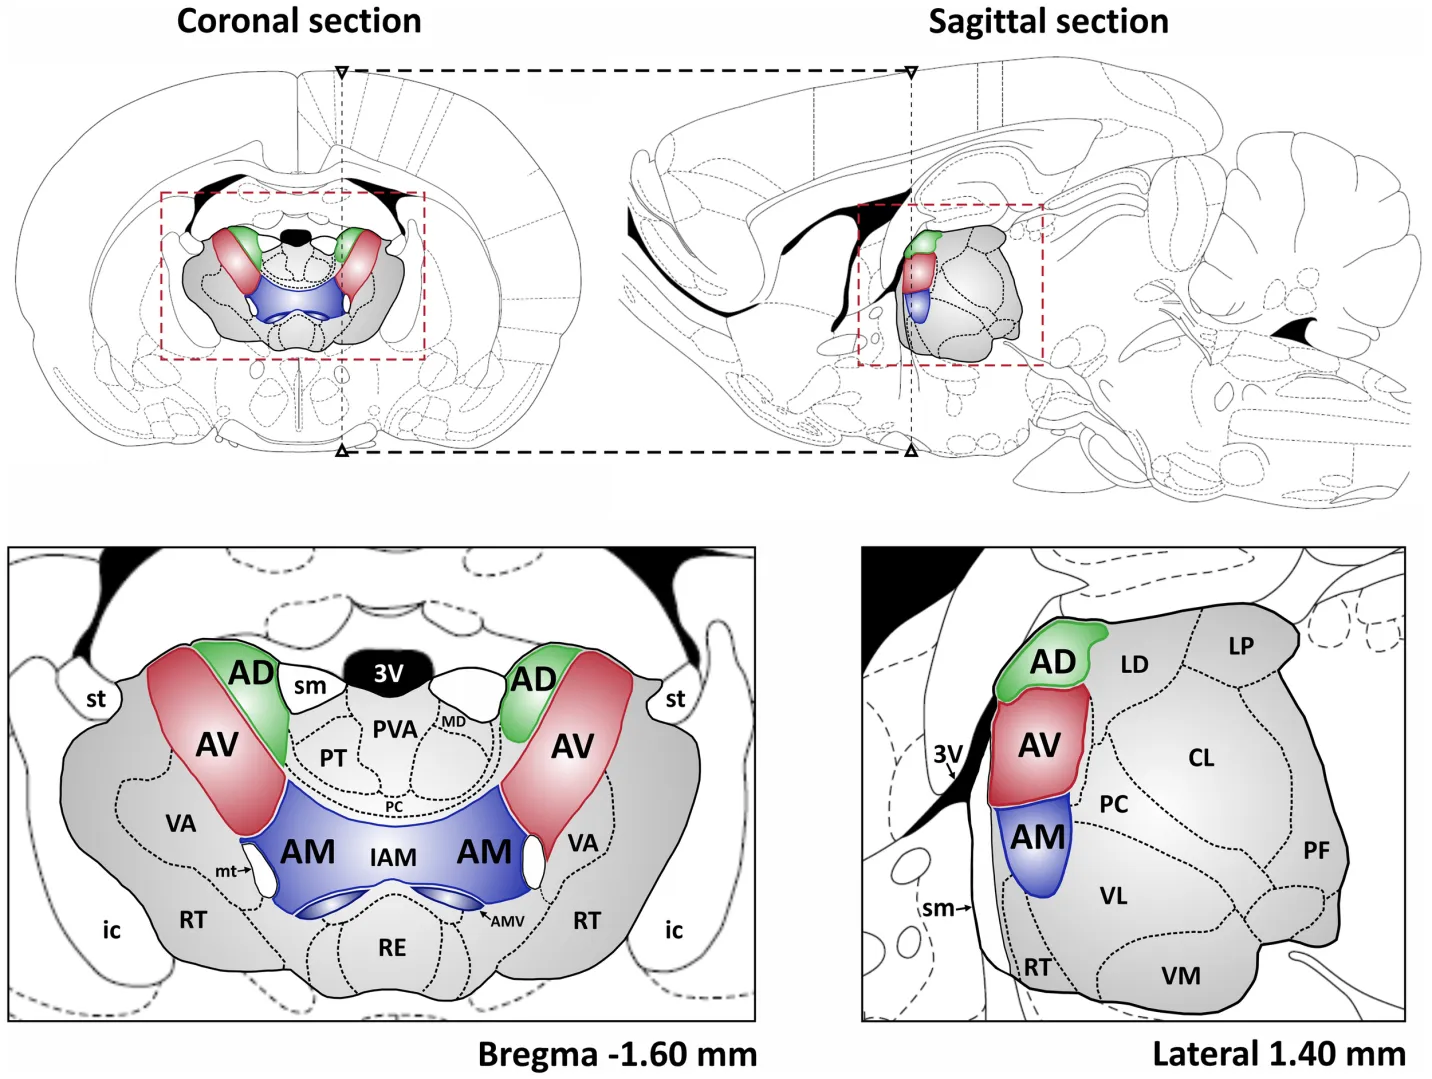
\includegraphics[width=0.8\linewidth]{fig1.5.png}
		\caption{The thalamus in mice.\cite{Jankowski2013}}
		\label{fig:The thalamus in mice}
	\end{figure}
	
	\begin{figure}[H]
		\centering
		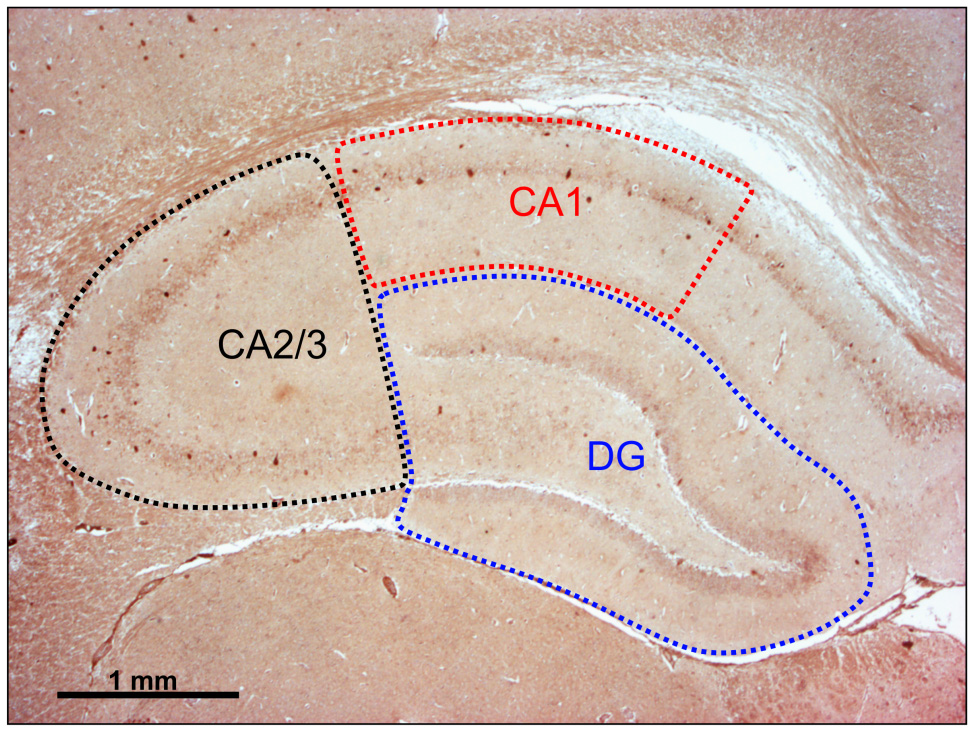
\includegraphics[width=0.8\linewidth]{fig1.6.png}
		\caption{The hippocampus in mice\cite{Selakovic2019}}
		\label{fig:The hippocampus in mice}
	\end{figure}
	%=======================
	\chapter{Review of Previous Studies}
	\label{chap:Review of Previous Studies}
	\section{Introduction}
	\label{Introduction2}
	This chapter begins with an overview of previous studies on global and local events. It then examines different types of phase-locking between sleep-related events and neuronal activity. Finally, the propagation of sleep spindles and slow oscillations in humans and mice is discussed.
	\section{Global and Local Events and Co-occurring Events}
	\label{Global and Local Events and Co-occurring Events}
	Yuval Nir and colleagues investigated slow oscillations during NREM sleep in 2012. Using EEG and depth EEG recordings obtained from the cortical and hippocampal regions of humans, they showed that most of these events were global\cite{Nir2011}. They also found a correlation between the amplitude of slow oscillations and their spatial extent. Specifically, the more widespread a slow oscillation was, the greater its amplitude.Figure~\ref{fig:global and local slow oscillation event} illustrates this relationship.\\
	Nir and colleagues defined a spindle or slow oscillation as local or global based on the proportion of recording sites in which the event was detected. If a spindle or slow oscillation was detected in fewer than 50\% of the recording sites, the event was considered local. In contrast, if it was detected in more than 50\% of the recording sites, it was classified as global.\\
	Figure~\ref{fig:global and local slow oscillation event} shows an example of a local slow oscillation event. As illustrated, an event can be observed in one brain region while being absent from another. Similar findings were also reported for sleep spindles.
	
	\begin{figure}[H]
		\centering
		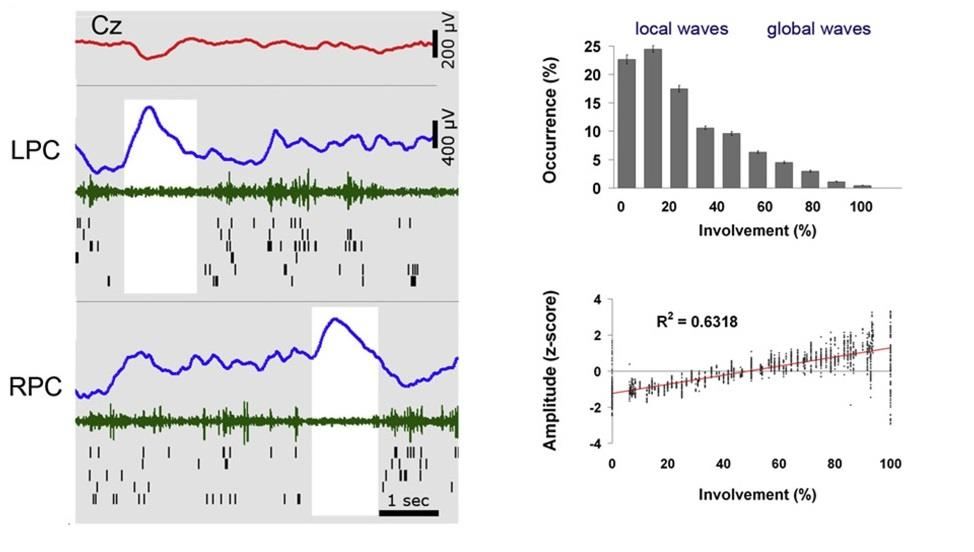
\includegraphics[width=0.8\linewidth]{fig2.1.png}
		\caption{Left: A global slow oscillation event. Top right: Histogram of slow oscillation events according to the percentage of recording regions in which they were detected. As shown, the majority of slow oscillations occurred in fewer than 50\% of the recording regions. Bottom right: Correlation plot between the normalized amplitude of slow oscillations and their spatial extent\cite{Nir2011}}
		\label{fig:global and local slow oscillation event}
	\end{figure}
	
	Most sleep spindles, like slow oscillations, were local. Moreover, larger-amplitude sleep spindles were more likely to be present across multiple recording regions (Figure~\ref{fig:global and local sleep spindles}).
	
	\begin{figure}[H]
		\centering
		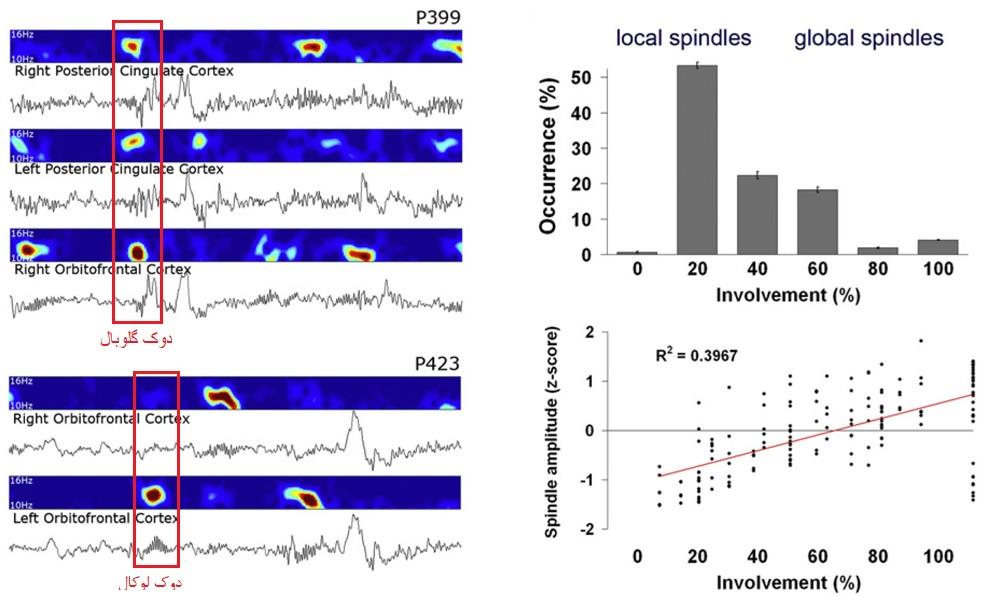
\includegraphics[width=0.8\linewidth]{fig2.2.png}
		\caption{Left: Examples of global and local sleep spindles in two patients. Top right: Distribution of sleep spindle events according to their presence across different recording regions. Most spindles were detected in fewer than 50\% of the recording regions and were therefore classified as local. Bottom right: Correlation between the normalized amplitude of sleep spindles and their presence across different recording regions. Higher spindle amplitudes were associated with a greater likelihood of the spindle being global.
			\cite{Nir2011}}
		\label{fig:global and local sleep spindles}
	\end{figure}
	
	By comparing the early and late periods of NREM sleep, the researchers also found that slow oscillations were present in fewer brain regions during the later periods of NREM sleep than during the earlier periods. This difference was statistically significant, indicating that slow oscillations became more local as NREM sleep progressed. In contrast, sleep spindles became more global during the later periods of NREM sleep compared with the earlier periods, and this increase in their presence across different brain regions was statistically significant (Figure~\ref{fig:Percentage of spindles present across different regions during the early and late periods of NREM sleep. Left: Same as the right panel, but for slow oscillations}).
	\begin{figure}[H]
		\centering
		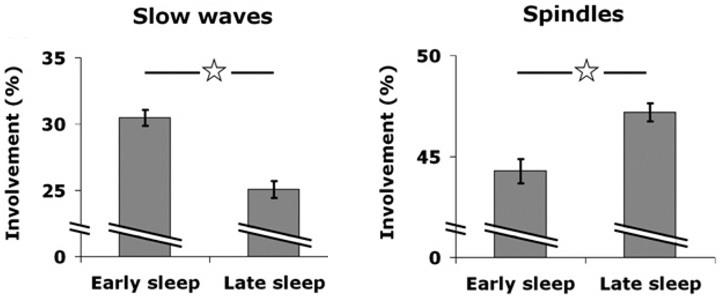
\includegraphics[width=0.8\linewidth]{fig2.3.png}
		\caption{Right: Percentage of spindles present across different regions during the early and late periods of NREM sleep. Left: Same as the right panel, but for slow oscillations\cite{Nir2011}}
		\label{fig:Percentage of spindles present across different regions during the early and late periods of NREM sleep. Left: Same as the right panel, but for slow oscillations}
	\end{figure}
	MakMcCully and colleagues showed in 2016, based on recordings obtained from humans\cite{MakMcCully2017}, that the occurrence of a slow oscillation in the cortex leads to a slow oscillation in the thalamus. Subsequently, interactions between the thalamus and the nucleus reticularis through repetitive cycles generate thalamic spindles, which in turn drive cortical spindles (Figure~\ref{fig:Relationship between slow oscillations and spindles in different regions}).
	\begin{figure}[H]
		\centering
		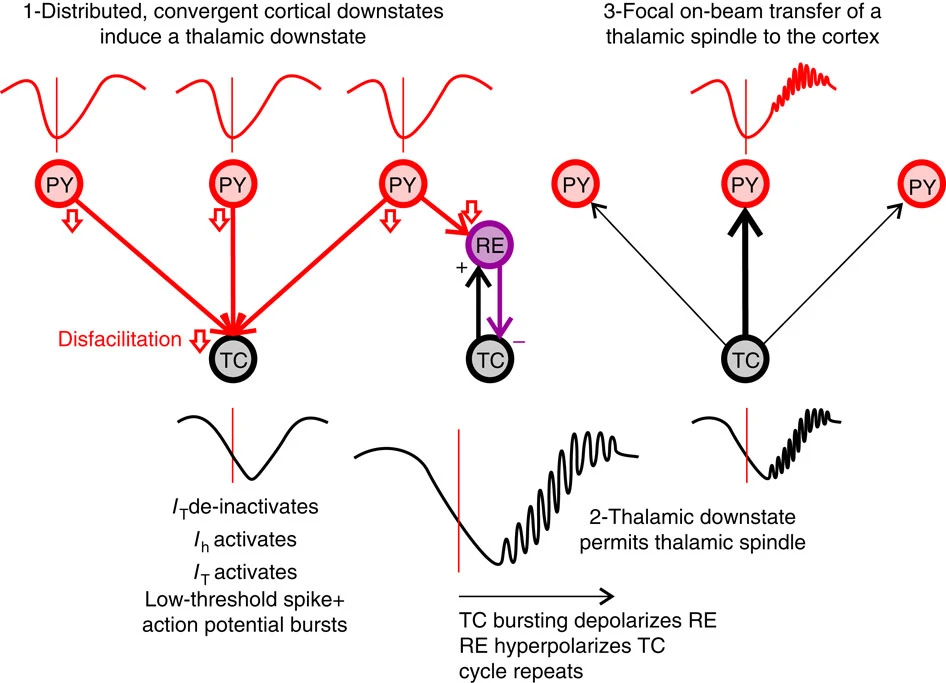
\includegraphics[width=0.8\linewidth]{fig2.4.png}
		\caption{Relationship between slow oscillations and spindles in different regions\cite{MakMcCully2017}}
		\label{fig:Relationship between slow oscillations and spindles in different regions}
	\end{figure}
	Piantoni and colleagues, in 2016, analyzed sleep recordings from six human subjects and observed that sleep spindles were present throughout the human cortex but exhibited a heterogeneous distribution. In other words, spindles did not occur with equal frequency across different cortical regions, and their local characteristics were influenced by the underlying cortical areas\cite{Piantoni2017}.
	They also showed that only a small proportion of spindles propagated across different cortical regions. In particular, spindles showed a greater tendency to co-occur between the superior temporal gyrus and lateral prefrontal cortex (Figure~\ref{Top: Co-occurring spindle distribution}).
	\begin{figure}[H]
		\centering
		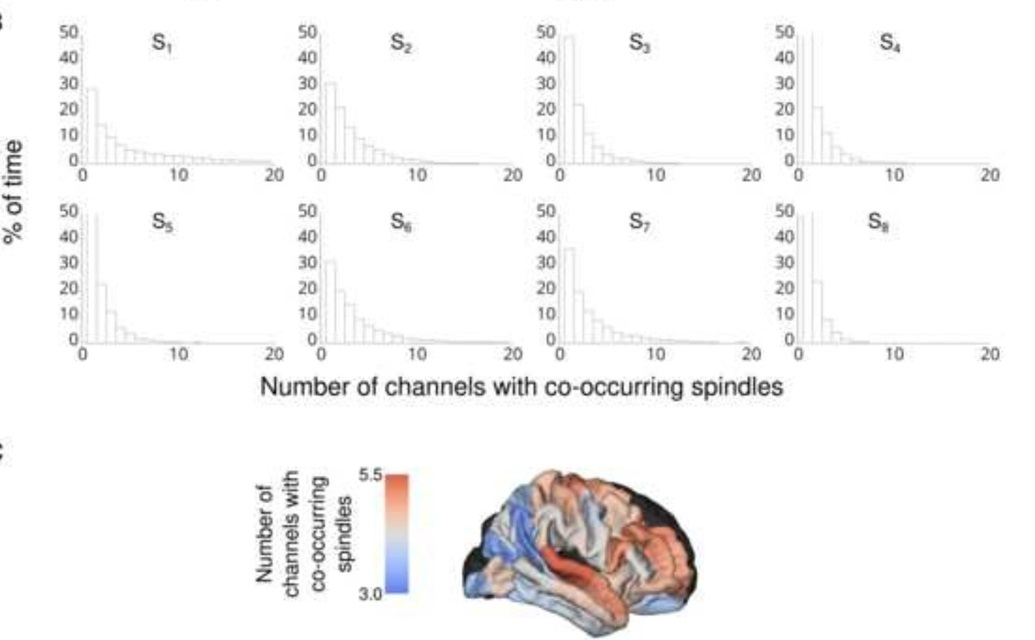
\includegraphics[width=0.8\linewidth]{fig2.5.jpg}
		\caption{Top: Percentage of time occupied by co-occurring spindle events across six different patients. Bottom: Number of channels exhibiting co-occurring spindles across different cortical regions.\cite{Piantoni2017}}
		\label{Top: Co-occurring spindle distribution}
	\end{figure}
	Bastoji and colleagues, in 2020, used simultaneous dual recordings from the thalamus and cortex in humans to investigate the spatial distribution of sleep spindles. They showed that 46\% of thalamic spindles were detected in only a single pair of contacts, suggesting that thalamic spindles have a more global distribution (Figure~\ref{fig:Thalamic spindle distribution by contact pairs})\cite{Bastuji2020}.\\
	The research team also showed that, for non-local thalamic spindles, corresponding spindles were present in other cortical regions where recordings were obtained. In contrast, for local thalamic spindles, corresponding spindles were not present across all recorded cortical regions (Figure~\ref{fig:Local and non-local thalamic spindles}).\\
	Furthermore, they found that, for local thalamic spindles, local cortical co-occurring spindles occurred significantly more frequently than non-local cortical co-occurring spindles. For non-local thalamic spindles, however, the occurrence of local and non-local cortical co-occurring spindles was approximately equal. Among the cortical regions, the highest percentage of co-occurring spindles with thalamic spindles was observed in the precuneus, whereas the lowest percentage was observed in the temporal (Temp) region (Figure~\ref{fig:Thalamocortical spindle characteristics}).
	
	\begin{figure}[H]
		\centering
		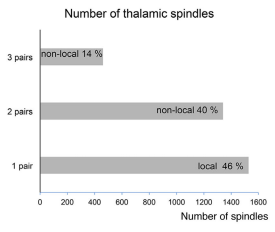
\includegraphics[width=0.8\linewidth]{fig2.6.png}
		\caption{Thalamic spindles according to the number of contact pairs in which they were detected.\cite{Bastuji2020}}
		\label{fig:Thalamic spindle distribution by contact pairs}
	\end{figure}
	
	\begin{figure}[H]
		\centering
		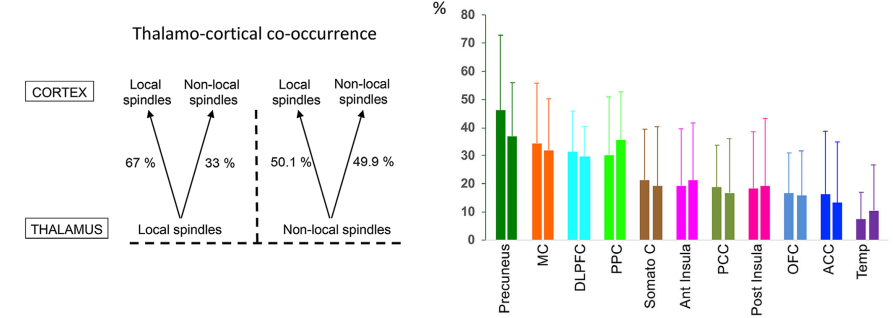
\includegraphics[width=0.8\linewidth]{fig2.8.png}
		\caption{Characteristics of thalamocortical spindles. Right: Percentage of local and non-local thalamic spindles associated with co-occurring spindles in each of the 11 cortical regions. Left: Local thalamic spindles had significantly more local than non-local cortical counterparts, whereas non-local thalamic spindles were associated with local and non-local cortical spindles at approximately equal proportions.\cite{Bastuji2020}}
		\label{fig:Thalamocortical spindle characteristics}
	\end{figure}
	
	\begin{figure}[H]
		\centering
		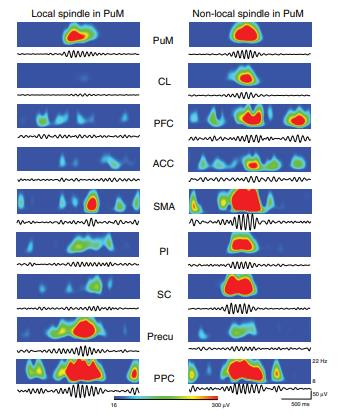
\includegraphics[width=0.8\linewidth]{fig2.7.png}
		\caption{Local (left) and non-local (right) thalamic spindles and their corresponding or non-corresponding spindles across different cortical regions.\cite{Bastuji2020}}
		\label{fig:Local and non-local thalamic spindles}
	\end{figure}
	
	\section{Phase-locking of sleep-related events with neuronal activity}
	Yuval Nir and colleagues showed in 2012 that there is a strong relationship between sleep slow waves in the EEG and the activity of single units across different brain structures\cite{Nir2011}. Although substantial variability was observed among neurons recorded from different brain regions, the activity of a considerable proportion of neurons was phase-locked to slow waves. Furthermore, the amplitude of EEG slow waves reflects the degree of modulation of neuronal activity; that is, greater slow-wave amplitudes are associated with stronger phase-locking (Figure~\ref{fig:Neuronal activity coupled to EEG slow waves}).
	\begin{figure}[H]
		\centering
		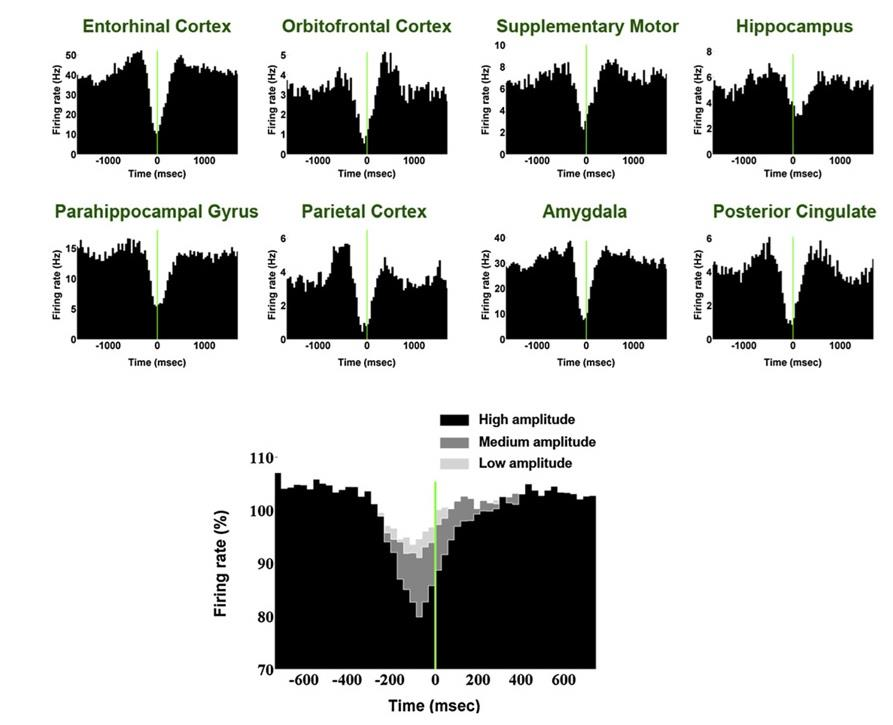
\includegraphics[width=0.8\linewidth]{fig2.9.png}
		\caption{Neuronal activity underlying EEG slow waves. Top: Examples of neurons recorded from different subjects and brain structures whose activity was strongly coupled to EEG slow waves. Bottom: Average unit waveforms across all brain structures as a function of the amplitude of positive EEG peaks. Slow waves were divided into three amplitude ranges; black, dark gray, and light gray represent high-, medium-, and low-amplitude slow waves, respectively.\cite{Nir2011}}
		\label{fig:Neuronal activity coupled to EEG slow waves}
	\end{figure}
	Dangoov Kim\cite{Kim2015} and colleagues, in 2015, recorded EEG signals from the cortex along with recordings from two electrodes implanted in the thalamus of mice \cite{Kim2015}. They then used K-means clustering to classify the detected spindles into three categories: global, posterior, and anterior spindles. They defined slow oscillations associated with spindles as those whose occurrence time ranged from $-0.8$ to $0.3$ s relative to spindle onset.
	
	They subsequently found that spindle-associated slow oscillations predominantly originated from anterior regions, regardless of spindle type. They also calculated the mean latency of the negative peak of the slow oscillations associated with each spindle type and found that this latency was greatest in the posterior region for all three spindle types (Figure~\ref{fig:Occurrence of spindle-associated slow waves}).
	\begin{figure}[H]
		\centering
		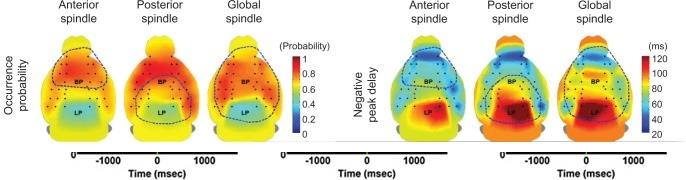
\includegraphics[width=0.8\linewidth]{fig2.10.png}
		\caption{Occurrence of spindle-associated slow waves. Left: Probability of occurrence. Right: Mean maps of the negative peak latency of slow waves associated with each spindle type.
			\cite{Kim2015}}
		\label{fig:Occurrence of spindle-associated slow waves}
	\end{figure}
	
	McCauley and colleagues, in a 2016 study of humans, demonstrated phase-locking between the timing of sleep spindles and the onset and offset of slow oscillations in the thalamus\cite{MakMcCully2017}. This phase-locking indicated that thalamic spindles typically occurred within the time interval between the onset and offset of the slow oscillation (Figure~\ref{fig:Thalamic spindle timing relative to DS}).
	\begin{figure}[H]
		\centering
		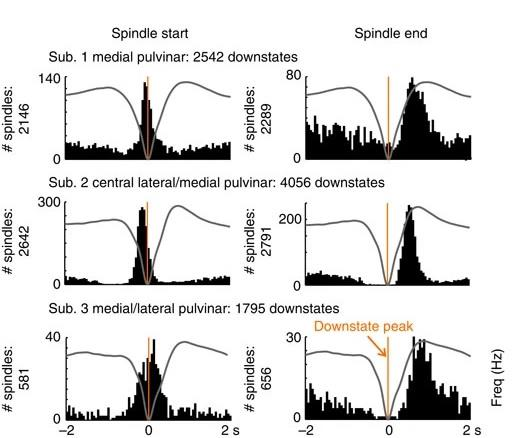
\includegraphics[width=0.8\linewidth]{fig2.11.png}
		\caption{Spindles typically begin around the thalamic DS peak and end near the subsequent positive peak. Histograms of thalamic spindle onset (first column) and spindle offset (second column) relative to the thalamic DS peak at zero (vertical orange line) for each thalamic channel.\cite{MakMcCully2017}}
		\label{fig:Thalamic spindle timing relative to DS}
	\end{figure}
	The research team also observed a similar phase-locking relationship between cortical spindles and cortical slow oscillations. Specifically, cortical spindles predominantly occurred between the down and up states of the slow oscillation. This finding was consistent across both slow and fast spindles (Figure~\ref{fig:Cortical spindle timing relative to DS}).
	\begin{figure}[H]
		\centering
		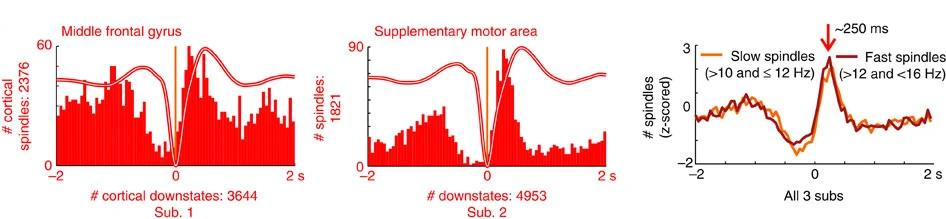
\includegraphics[width=0.8\linewidth]{fig2.12.png}
		\caption{Left: Histogram of cortical spindle onset relative to the cortical DS peak at 0 (vertical orange line). Right: Both slow and fast spindles occur during the transition from the down state to the up state.\cite{MakMcCully2017}}
		\label{fig:Cortical spindle timing relative to DS}
	\end{figure}
	Bandarabadi and colleagues, in 2020, used LFP recordings obtained from the cortex and thalamus of mice and demonstrated phase-locking between neuronal activity and sleep spindles across the different brain regions examined\cite{Bandarabadi2020}.
	Their findings showed that the activity of TRN\footnote{ thalamic reticular nucleus} units was strongly phase-locked to LFP spindle cycles. They also found that spike-phase locking in the CMT\footnote{centromedial} and AD\footnote{anterodorsal} thalamic nuclei was as strong as that observed in the TRN during spindles. Neurons in the CING\footnote{anterior cingulate} and VB\footnote{ventrobasal complex of the thalamus} regions showed an increase in activity only around the spindle peaks, whereas BARR\footnote{barrel cortex} cells exhibited an inverse phase-locking pattern, with most neuronal spikes occurring near the troughs. In the VIS\footnote{Visual cortex} cortex, neuronal activity was only weakly coupled to LFP oscillations during spindles (Figure~\ref{fig:Cellular substrates of sleep spindles}).
	To quantitatively assess and compare the degree of phase-locking, they also examined a measure referred to as spike–field coupling. To quantify spike–field coupling, they calculated the normalized cross-correlation between the average filtered LFP signals and the mean firing rate during spindles. Statistical comparisons showed that the observed increase in phase-locking in the TRN was significant compared with the CING, BARR, VIS, and VB regions, whereas no significant difference was observed compared with the CMT and AD regions (Figure~\ref{fig:Spike–field coupling during spindles}).
	They subsequently investigated the relationship between spindles and slow oscillations across all recorded regions (Figure~\ref{fig:Time–frequency representation of sleep spindles}). They quantified SO–spindle coupling using the normalized cross-correlation between the mean traces and found significant SO–spindle phase-locking in the CING, CMT, and AD regions compared with the VIS, BARR, VB, TRN, and EEG recordings.
	They further calculated the percentage of spindles that coincided with the up states of slow oscillations. Consistent with the SO–spindle coupling results, spindles in the AD, CMT, and CING regions showed a significantly higher proportion of occurrence during the up states compared with the other regions (Figure~\ref{fig:SO–spindle coupling and spindle occurrence during up states}).
	
	\begin{figure}[H]
		\centering
		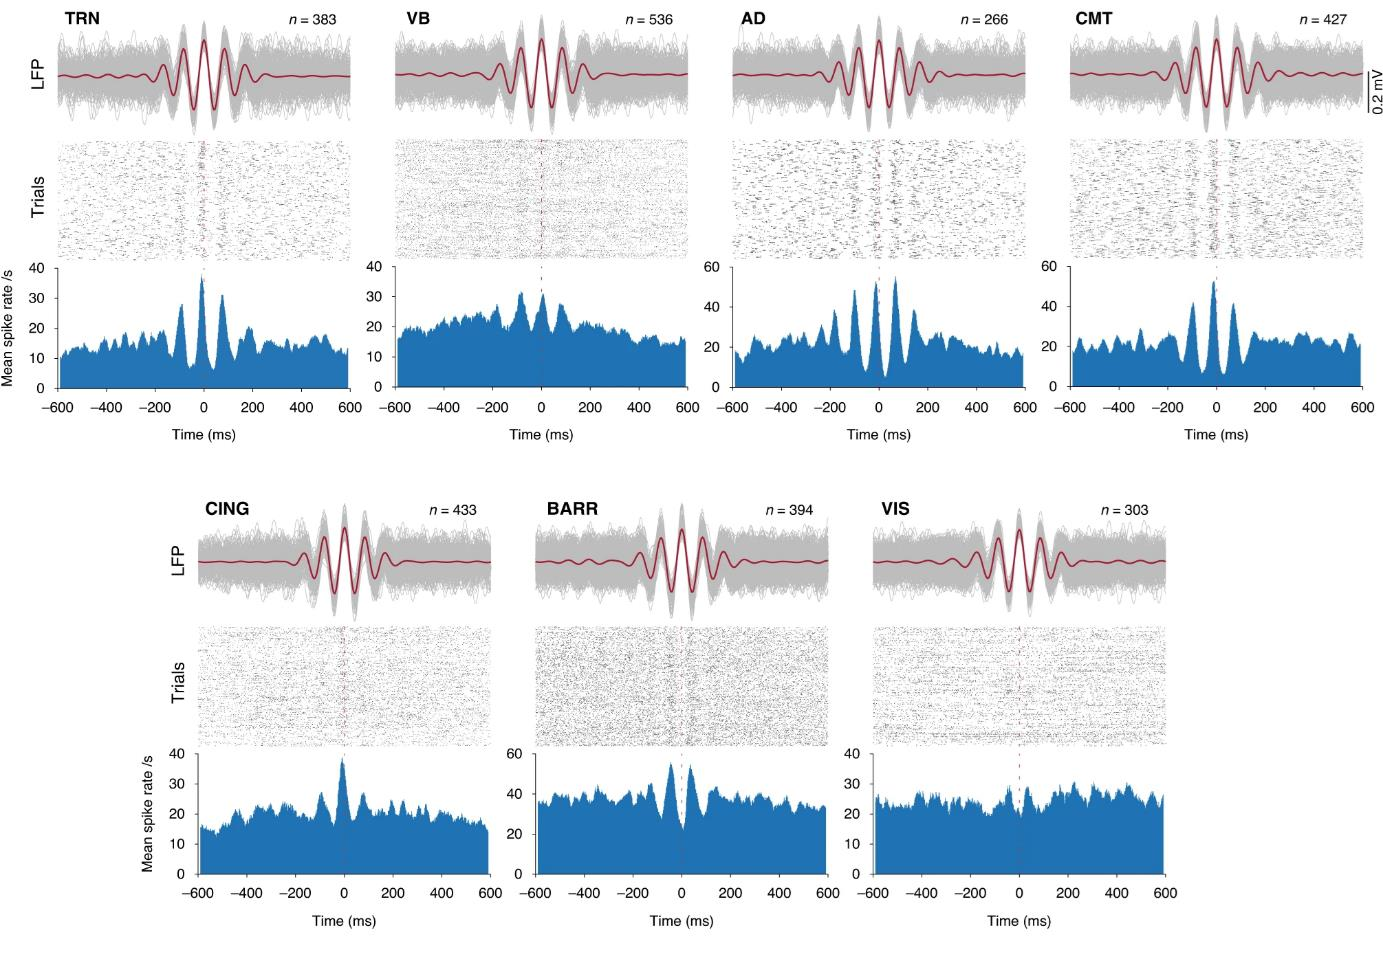
\includegraphics[width=0.8\linewidth]{fig2.13.png}
		\caption{Cellular substrates of sleep spindles in the thalamic nucleus and cortex. The mean thalamic spindle (red) and individual spindles (gray) are shown. Raster plots illustrate the activity of each thalamic neuronal unit during spindles.\cite{Bandarabadi2020}}
		\label{fig:Cellular substrates of sleep spindles}
	\end{figure}
	\begin{figure}[H]
		\centering
		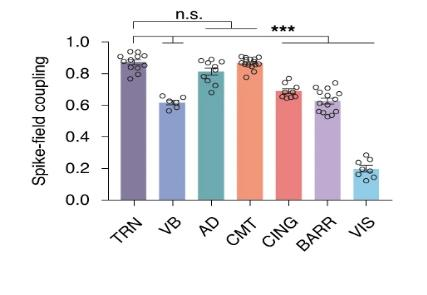
\includegraphics[width=0.8\linewidth]{fig2.14.png}
		\caption{Spike–field coupling during spindles using normalized cross-correlation.\cite{Bandarabadi2020}}
		\label{fig:Spike–field coupling during spindles}
	\end{figure}
	\begin{figure}[H]
		\centering
		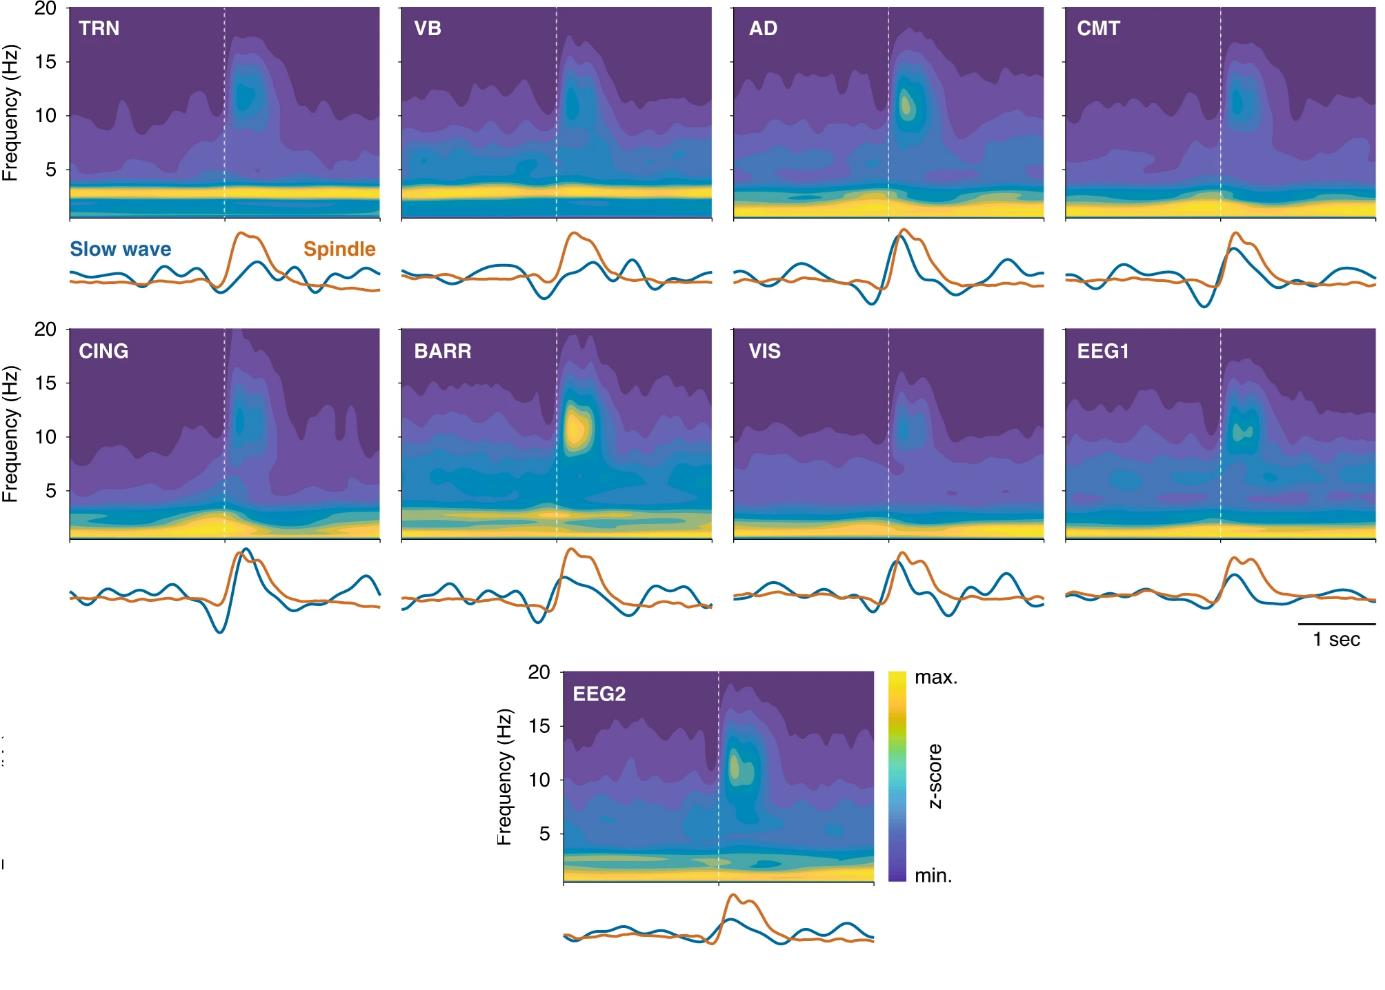
\includegraphics[width=0.8\linewidth]{fig2.15.png}
		\caption{The plots show the average time–frequency representation of sleep spindles. The vertical white dashed lines indicate spindle onset. The plots below the spectrograms show the average filtered LFPs for the SO (blue) and the average LFPs filtered within the spindle frequency range (red).\cite{Bandarabadi2020}}
		\label{fig:Time–frequency representation of sleep spindles}
	\end{figure}
	\begin{figure}[H]
		\centering
		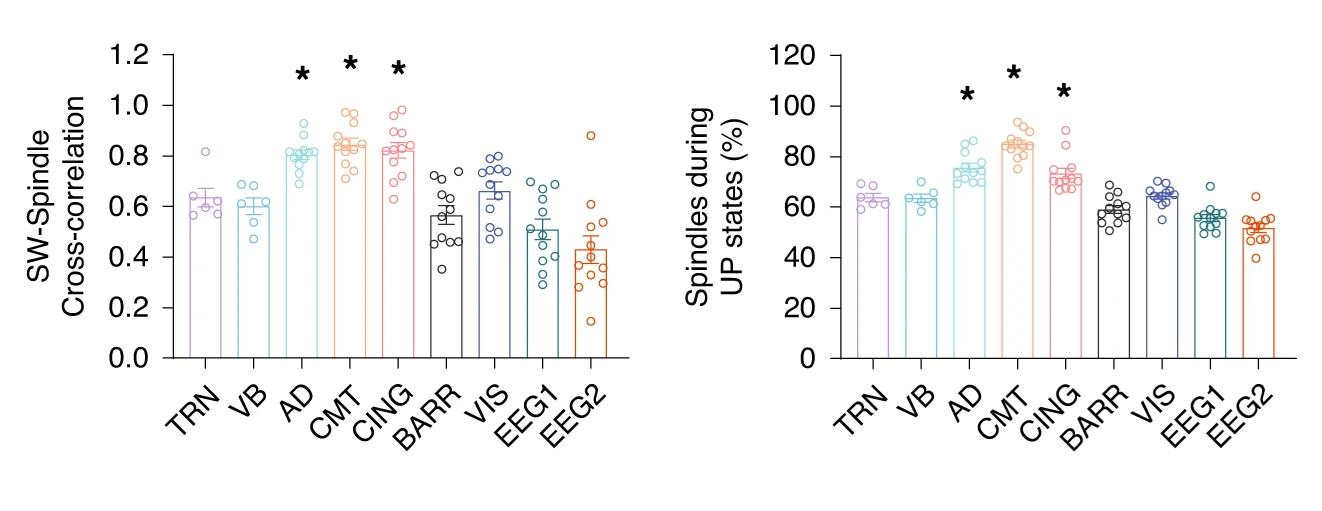
\includegraphics[width=0.8\linewidth]{fig2.16.png}
		\caption{Left: Normalized cross-correlation between SOs and spindles, indicating significant SO–spindle coupling in the CING, CMT, and AD regions compared with the other regions. Right: Percentage of spindles coinciding with the up states. The proportions of spindles occurring during the up states were significantly higher in the AD, CMT, and CING regions than in the other regions.\cite{Bandarabadi2020}}
		\label{fig:SO–spindle coupling and spindle occurrence during up states}
	\end{figure}
	Charles D. et al. showed in 2021\cite{Dickey2021}, using LFP recordings obtained from the human cortex, that neuronal activity is directly related to sleep spindles. They classified spindles into two categories: isolated spindles and spindles coupled to either the up or down states of slow oscillations. They also examined neuronal activity in two different types of units, PY\footnote{pyramidal cells} and IN\footnote{interneuron}.
	
	They subsequently found that neuronal co-firing was higher when all co-occurring spindles were considered than during periods without any spindles. Co-firing increased again during isolated spindles. Similarly, co-firing was strongly increased for units associated with spindles coupled to either the up or down states of slow oscillations. These results were similar for both PY and IN units (Figure~\real{fig:Pairwise neuronal co-firing during spindles}).
	
	The research team further showed that the delay in the co-firing of spatially co-localized neurons was linearly related to the phase delay of co-occurring spindles (Figure~\ref{fig:Co-firing as a function of spindle phase delay}).
	\begin{figure}[H]
		\centering
		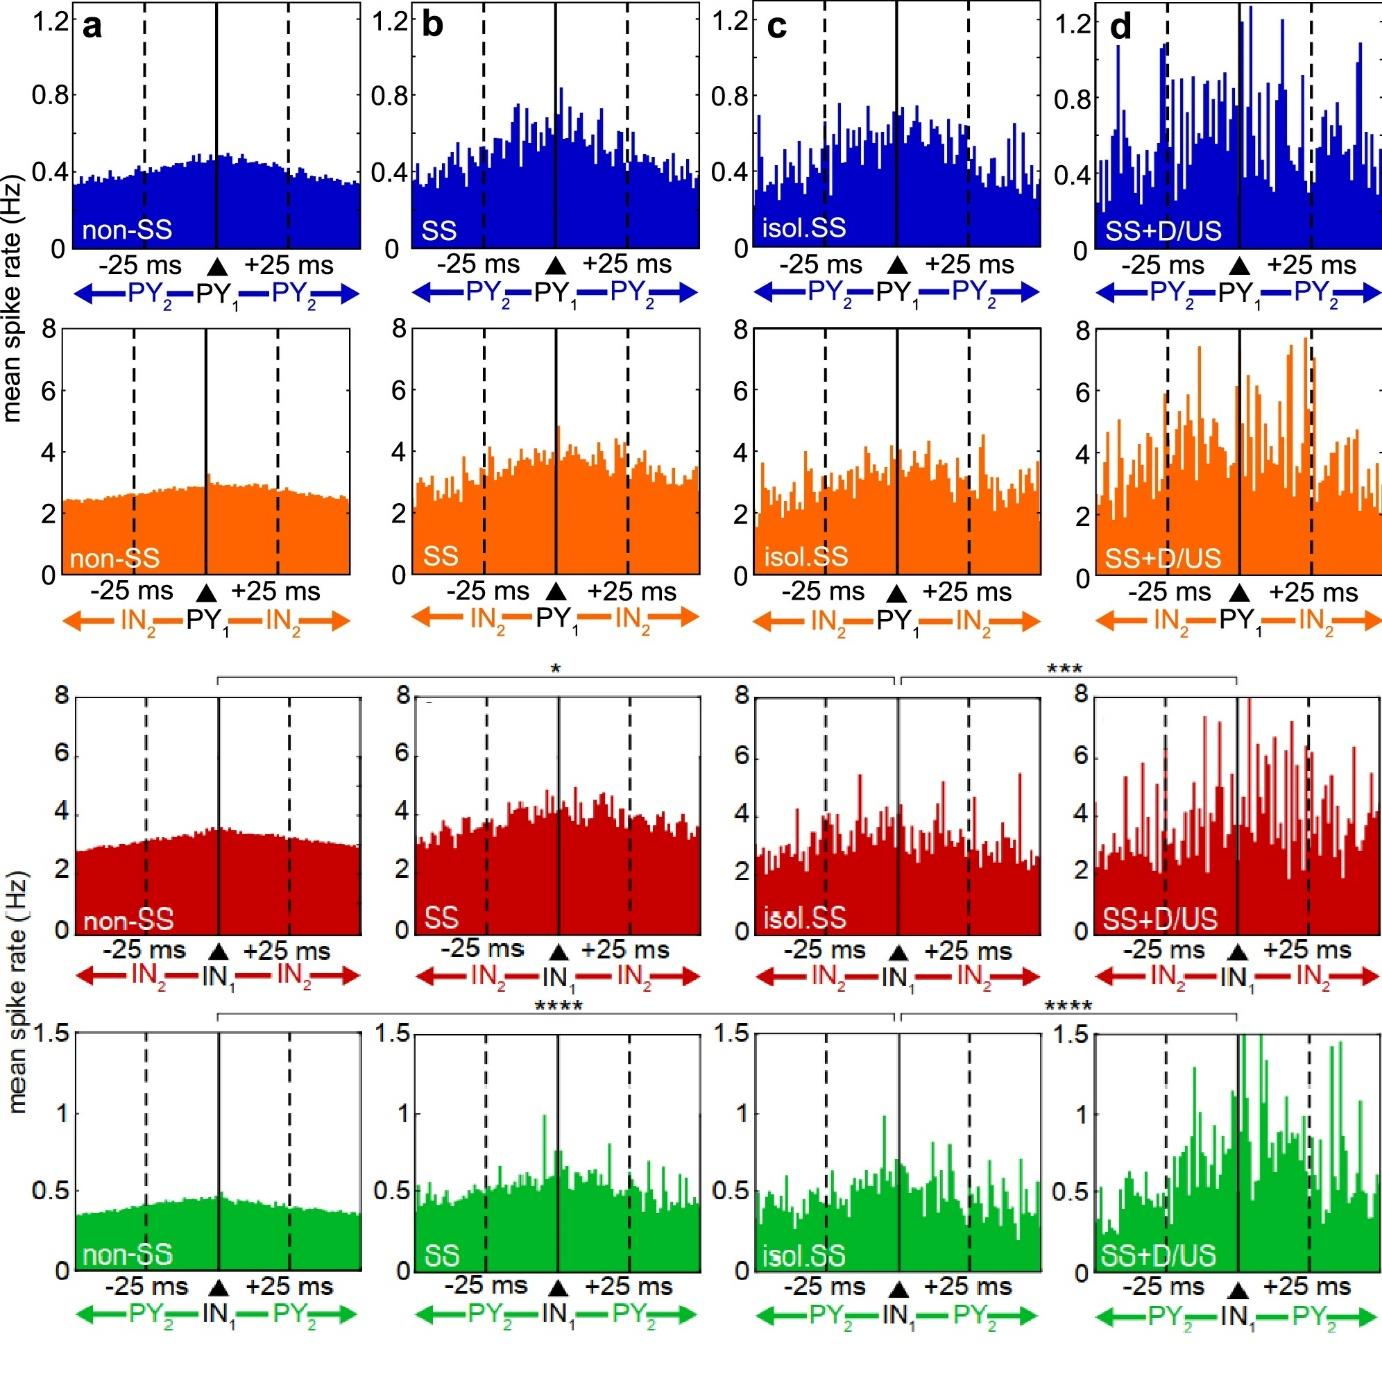
\includegraphics[width=0.8\linewidth]{fig2.17.png}
		\caption{Pairwise neuronal co-firing during spindles. (a) Non-spindle periods (baseline), (b) co-occurring spindles, (c) spindles not coupled to the up/down states, and (d) co-occurring spindles coupled to the up/down states\cite{Dickey2021}}
		\label{fig:Pairwise neuronal co-firing during spindles}
	\end{figure}
	\begin{figure}[H]
		\centering
		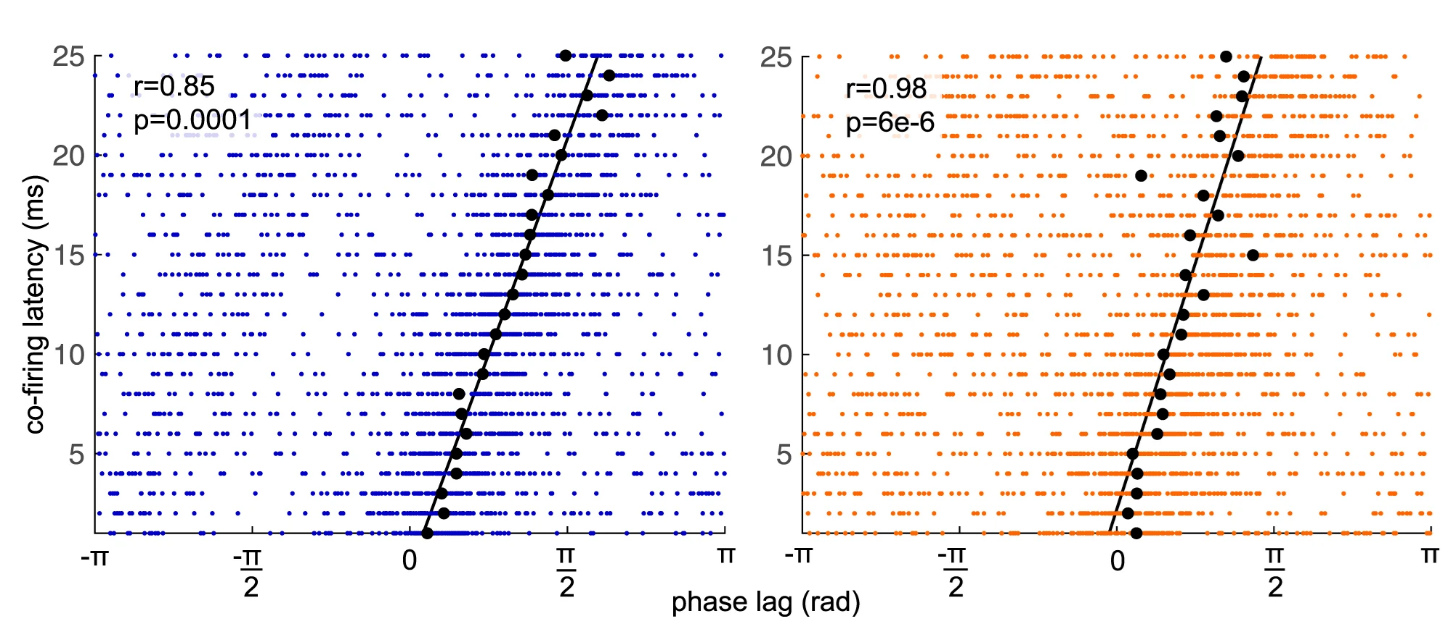
\includegraphics[width=0.8\linewidth]{fig2.18.png}
		\caption{Pairwise co-firing within 25 ms as a function of spindle phase delay. Black circles represent the circular mean for each 1-ms delay, and the black line represents the best circular–linear fit to these means. The P-value indicates the significance of the correlation coefficient.\cite{Dickey2021}}
		\label{fig:Co-firing as a function of spindle phase delay}
	\end{figure}
	Noam Nitzan and colleagues, in 2022\cite{Nitzan2022}, analyzed a dataset obtained from different brain regions, including the hippocampus, cortex, and thalamus. They showed that neuronal activity changed within a limited time window before and after sharp-wave ripples (SPW-Rs). In the CN\footnote{cerebral nuclei} region, neuronal activity increased during the interval surrounding SPW-Rs and was followed by a subsequent decrease in neuronal activity. In contrast, neuronal activity in the TH\footnote{thalamus} region decreased before the occurrence of SPW-Rs and increased after the SPW-Rs (Figure~\ref{fig:SPW-R-related activity across extrahippocampal regions}).
	\begin{figure}[H]
		\centering
		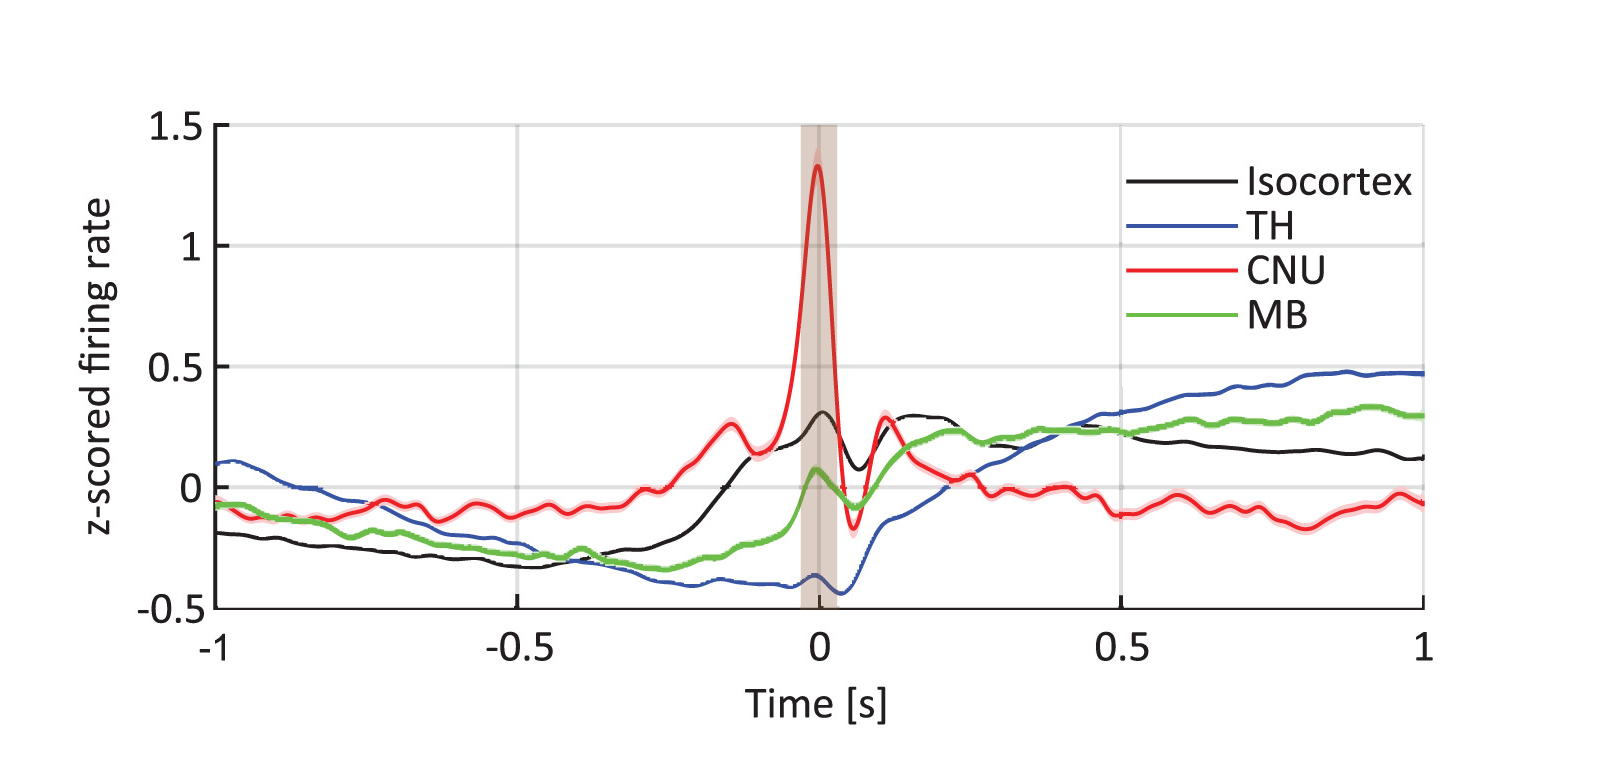
\includegraphics[width=0.8\linewidth]{fig2.19.png}
		\caption{Mean (mean ± SEM) SPW-R-related activity across four major extrahippocampal regions: TH, MB, CN, and isocortex\cite{Nitzan2022}}
		\label{fig:SPW-R-related activity across extrahippocampal regions}
	\end{figure}
	Peyrache and colleagues, in 2012\cite{Peyrache2011}, used recordings obtained from the mouse cortex to investigate neuronal activity in two cortical layers, superficial and deep, for fast-spiking (FS) and regular-spiking (RS) cells. They showed that neuronal activity during spindle events increased significantly in neurons located in the deep layer. In addition, neurons in the superficial layer tended to fire at the spindle peaks. This tendency was also observed in neurons in the deep layer, although to a lesser extent (Figure~\ref{fig:Neuronal firing and phase modulation during sleep spindles}).
	
	\begin{figure}[H]
		\centering
		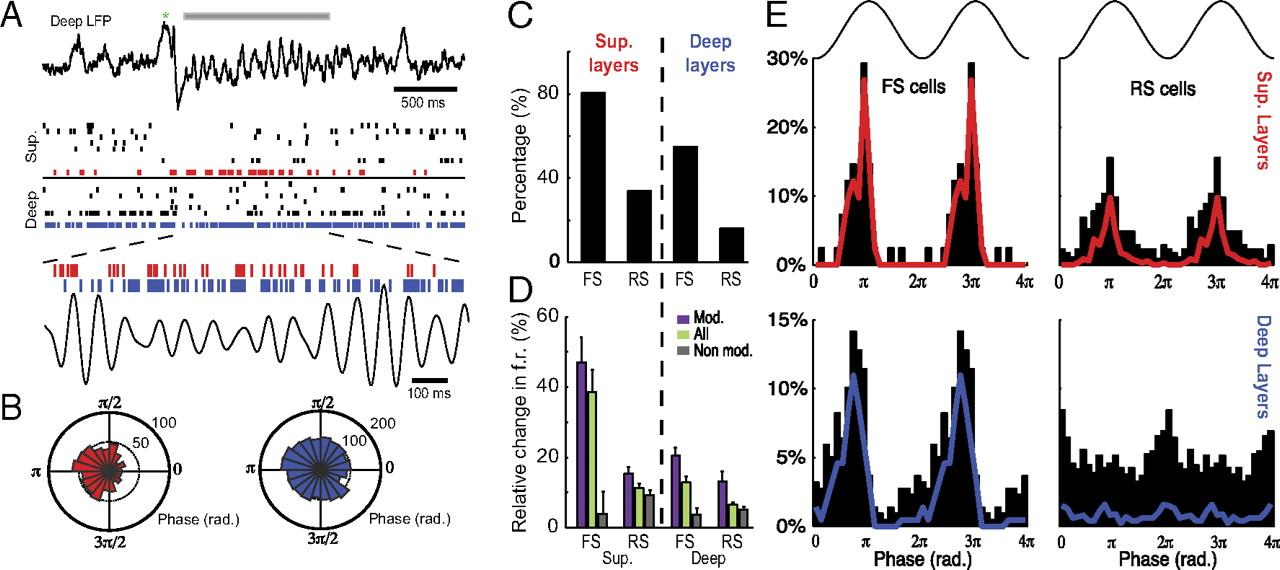
\includegraphics[width=0.8\linewidth]{fig2.20.png}
		\caption{Firing of superficial pyramidal cells and neurons during spindles. (A) Raw deep LFP signal (top), with the spindle indicated by the horizontal gray bar. Below: Raster plot of individual units showing spike activity in the superficial (II/III) and deep (V/VI) layers. Firing from two FS cells, one in each layer, is shown in color, whereas spikes from RS cells are shown in black. Bottom: Enlarged view of a spindle oscillation. (B) Phase histogram of FS cells. (C) Percentage of cells showing significant phase modulation. (D) Mean relative change in firing rate over the spindle oscillation compared with non-spindle SWS for significantly phase-locked cells (purple), non-phase-locked cells (gray), and all cells (green). Error bars represent SEM. (E) Distribution of the preferred firing phase of cells. Black bars indicate the preferred phase for all cells. The distribution for significantly phase-modulated cells is shown only for the colored traces\cite{Peyrache2011}}
		\label{fig:Neuronal firing and phase modulation during sleep spindles}
	\end{figure}
	The research team also showed that, in neurons from both cortical layers, changes in the firing rate were greater when the neurons were modulated by spindles than when no spindle modulation was present. This finding was observed for both FS and RS cells (Figure~\ref{fig:Neuronal firing and phase modulation during sleep spindles}).
	
	Another finding was that, with the exception of RS cells in the deep layer, neurons in the other regions and cell types showed a strong tendency to fire at spindle peaks (Figure~\ref{fig:Neuronal firing and phase modulation during sleep spindles}).
	
	Furthermore, the research team showed that neuronal responses to slow waves (SWs) during periods without spindles were greater than those during periods accompanied by spindles. This finding was observed in both cortical layers and for FS cells (Figure~\ref{fig:Cellular responses to SPW-Rs during spindles}).\\
	Alizadeh and colleagues, in 2022\cite{Alizadeh2022}, used simultaneously recorded data from the thalamus and hippocampus of mice and showed that neuronal activity around slow spindle–associated ripple events was greater than that observed during ripples occurring alone or ripples occurring together with fast spindles. The dataset used by this group also included a behavioral task (Task 1). Therefore, neuronal activity before and after exploration of the experimental environment was also examined. The results showed that the mean firing rate of CA1/AD neurons did not change significantly between sleep periods before and after exploration. However, during post-exploration sleep periods, CA1 units were strongly modulated by spindles compared with pre-exploration sleep (Figure~\ref{fig:Neuronal activity during thalamic spindles}).
	
	\begin{figure}[H]
		\centering
		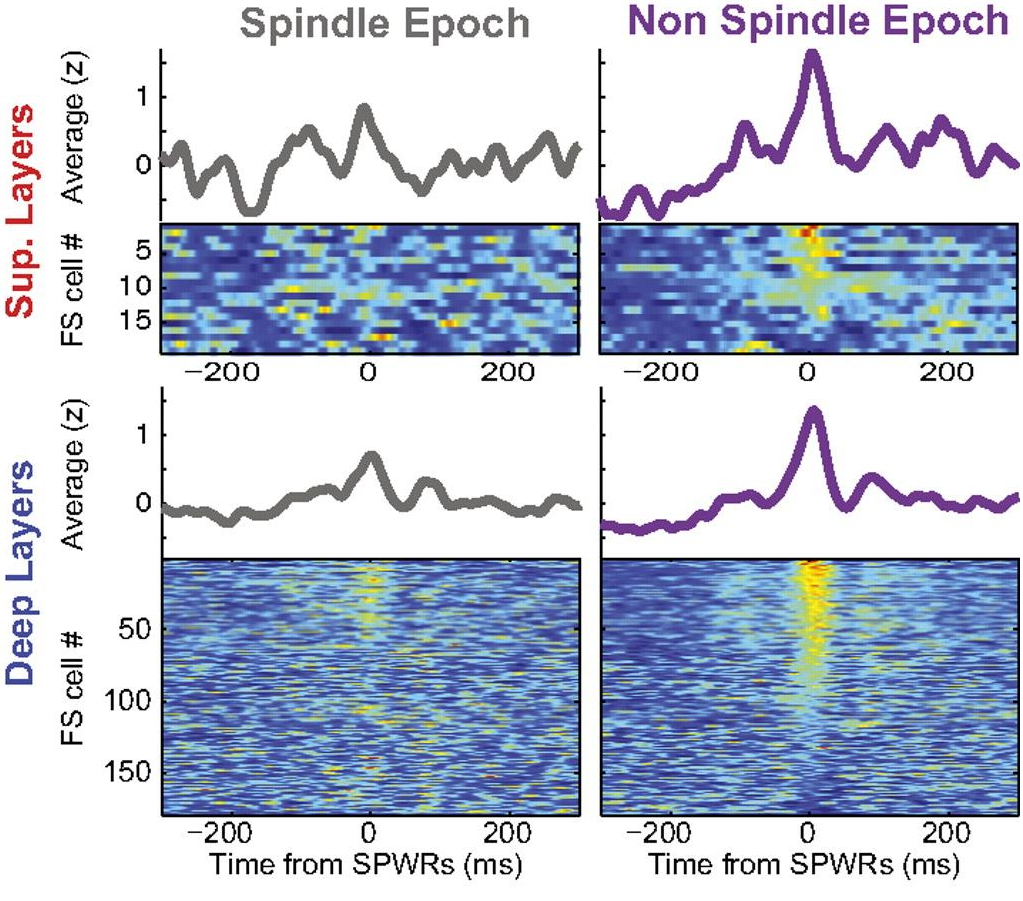
\includegraphics[width=0.8\linewidth]{fig2.21.png}
		\caption{Cells increased their responsiveness to hippocampal SPW-Rs during spindle periods compared with non-spindle periods. Mean (top) and individual (bottom) responses of superficial FS cells relative to the time of SPW-R occurrence during spindle oscillations (left) and non-spindle periods (right)\cite{Peyrache2011}}
		\label{fig:Cellular responses to SPW-Rs during spindles}
	\end{figure}
	
	\section{Propagation of Brain Waves and Sleep Events}
	\label{sec:Propagation of Brain Waves and Sleep Events}
	Yuval Nir and colleagues, in 2012\cite{Nir2011}, showed that slow oscillations tend to propagate from the medial frontal cortex toward the hippocampus. They also found that this propagation tendency follows the expected anatomical pathway (Figure~\ref{fig:Slow-wave propagation along anatomical pathways}).\\
	Dangoov Kim and colleagues, in 2015\cite{Kim2015}, used EEG recordings from the cortex and LFP recordings from the thalamus of mice to show that slow oscillations originated predominantly in the anterior region of the brain and could be observed across all brain regions. These observations suggest that slow oscillations propagate from the anterior toward the posterior regions (Figure~\ref{fig:Propagation Topography of Slow Oscillations}).\\
	Piantoni and colleagues, in 2016\cite{Piantoni2017}, based on cortical recordings obtained from humans, showed that sleep spindles tend to propagate from the superior frontal and temporal regions toward the orbitofrontal cortex. For co-occurring spindles detected in two different regions, the researchers defined a ratio based on whether the spindle was classified as leading or lagging. They found that spindle propagation from the superior frontal and temporal regions toward the orbitofrontal cortex occurred with ratios greater than 2:1 (Figure~\ref{fig:Directional propagation of sleep spindles}).
	\begin{figure}[H]
		\centering
		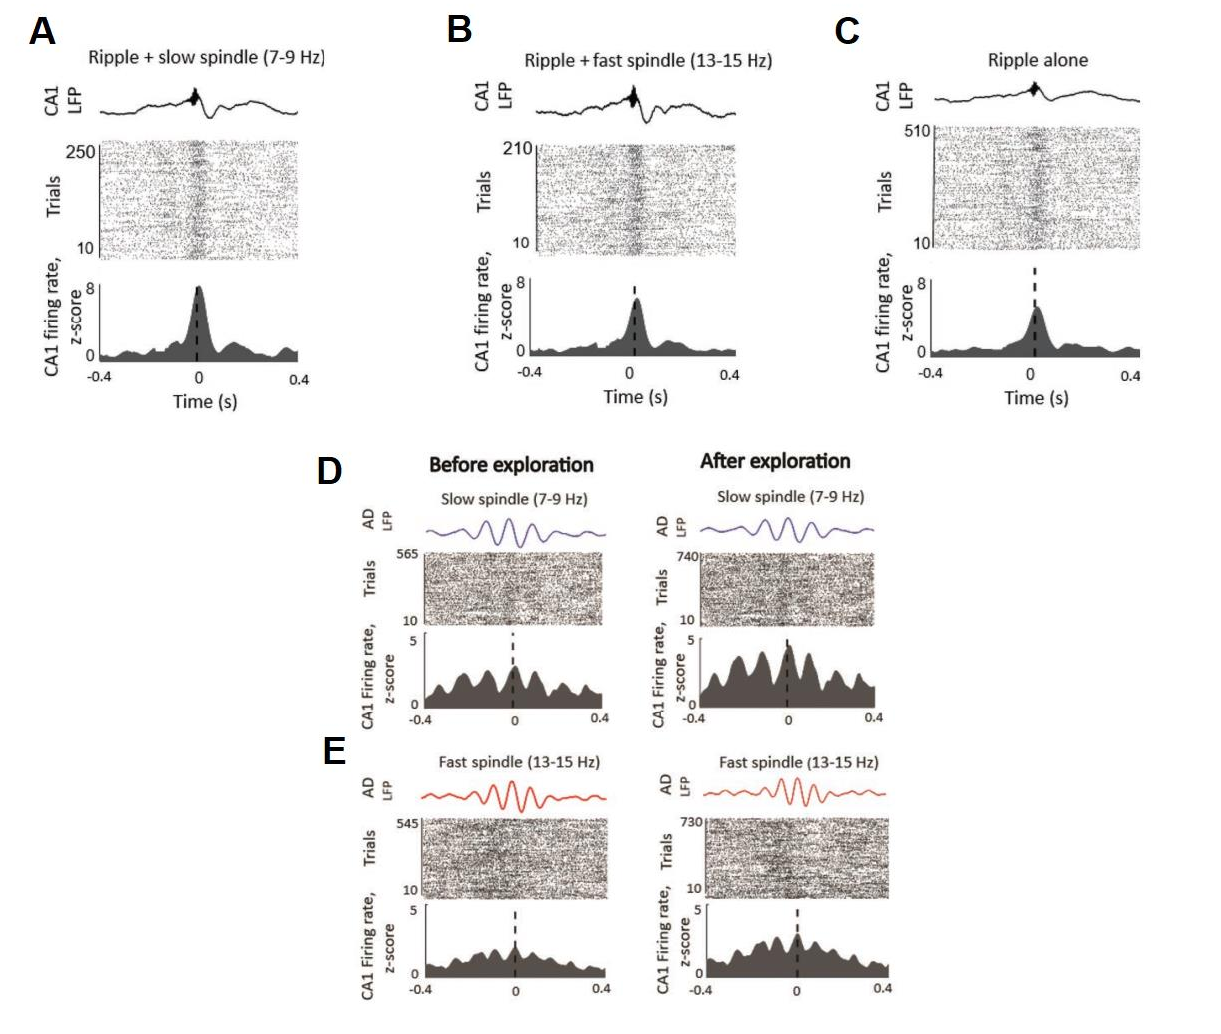
\includegraphics[width=0.8\linewidth]{fig2.22.png}
		\caption{(A) Top: Mean raw CA1 LFP aligned to the peaks of waves co-occurring with slow thalamic spindles (7–9 Hz). Middle: Spike rasters, and bottom: peri-ripple peak histograms of CA1 spikes during spindle oscillations (left) and non-spindle periods (right). (E, F) Same as (A), but for waves co-occurring with fast thalamic spindles (13–15 Hz) and isolated ripples, respectively. (D) Top: Mean AD LFP filtered in the slow spindle frequency range (7–9 Hz) and aligned to slow spindle peaks. Middle: Time-aligned raster plots, and bottom: histograms of activity around slow spindles before (left) and after (right) exploration. (E) Same as (D), but for fast spindles (13–15 Hz) [8]\cite{Alizadeh2022}}
		\label{fig:Neuronal activity during thalamic spindles}
	\end{figure}
	\begin{figure}[H]
		\centering
		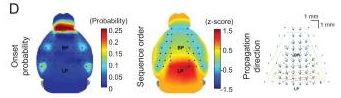
\includegraphics[width=0.8\linewidth]{fig2.24.png}
		\caption{Topography of slow oscillation propagation. Left: Topography of the probability of slow oscillation onset, with the highest probability observed in the frontal region. Middle: Z-score map of slow oscillations showing the expected occurrence of a slow wave across different brain regions. Right: Direction of slow oscillation propagation\cite{Kim2015}}
		\label{fig:Propagation Topography of Slow Oscillations}
	\end{figure}
	\begin{figure}[H]
		\centering
		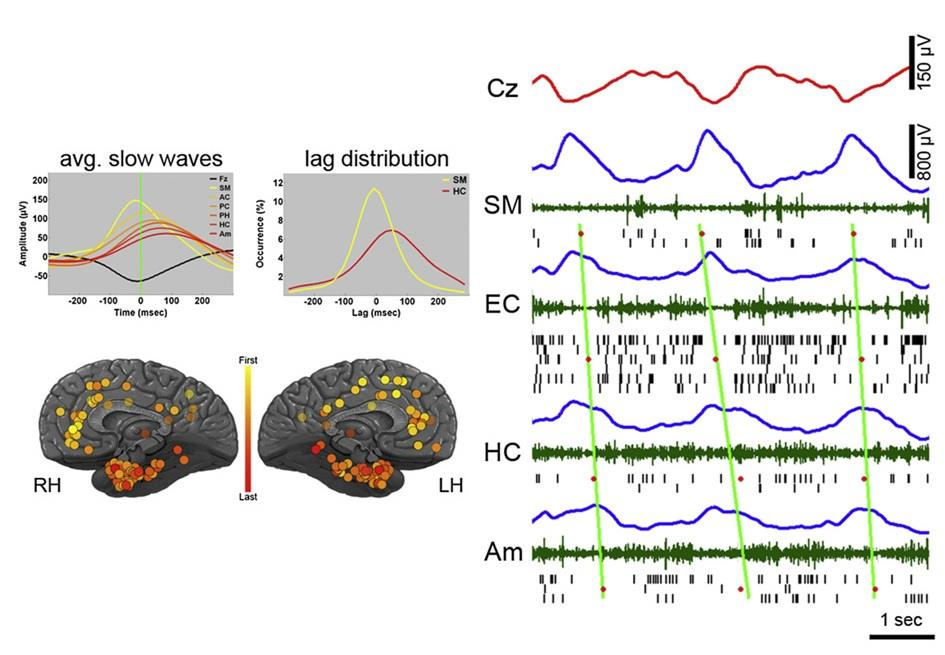
\includegraphics[width=0.8\linewidth]{fig2.23.png}
		\caption{Propagation of slow sleep waves along anatomical pathways. Top left: Topography of the onset probability of slow waves. The highest probability is located in the frontal cortex. Center: Z-score map of slow waves showing the expected occurrence of a slow wave across different brain regions. Bottom left: Mean propagation trajectory of slow waves. Each circle represents a depth electrode according to its precise anatomical location. Yellow-to-red colors indicate waves that occurred earlier in the frontal cortex than in the MTL. Right: Example of slow waves propagating from the frontal cortex to the MTL. From top to bottom, the rows show scalp EEG (Cz, red), supplementary motor area (SM), entorhinal cortex (EC), hippocampus (HC), and amygdala (Am). Colors indicate the following: blue, depth EEG; green, MUA; and black lines, clusters of isolated units. Red dots indicate the center of OFF periods in each brain region. Green diagonal lines are fitted to the OFF-period times using linear regression and indicate the direction of propagation\cite{Nir2011}}
		\label{fig:Slow-wave propagation along anatomical pathways}
	\end{figure}
	Dickey and colleagues, in 2021\cite{Dickey2021}, recorded neural activity from the cortex of four patients using a Utah array. The research team showed that, at a spatial scale of less than one centimeter, spindles propagated across the array. The propagation initially followed a circular pattern up to the spindle peak and then continued in a linear pattern after the peak (Figure~\ref{fig:Sub-centimeter spindle propagation}). A video of this propagation is available at the website provided in Footnote\footnote{\href{https://media.springernature.com/original/springer-static/esm/art\%3A10.1038\%2Fs41467-021-21298-x/MediaObjects/41467\_2021\_21298\_MOESM4\_ESM.mov}{https://media.springernature.com/original/springer-static/esm/art\%3A10.1038\%2Fs41467-021-21298-x/MediaObjects/41467\_2021\_21298\_MOESM4\_ESM.mov}}.
	
	Nithard and colleagues, in 2018\cite{Niethard2018}, used EEG recordings obtained from the brains of mice and showed that slow oscillation-related activity exhibited a systematic propagation from the frontal region toward the occipital cortical region. Specifically, the decrease in activity during the negative half-wave reached its peak slightly earlier in the frontal cortical regions than in the posterior regions. This propagation pattern was observed for both slow oscillations and slow oscillation events coupled with sleep spindles (Figure~\ref{fig:Frontal-to-posterior SO propagation}). A video of this propagation is available on the website provided in Footnote\footnote{\href{ http://movie-usa.glencoesoftware.com/video/10.1073/pnas.1805517115/video-1}{ http://movie-usa.glencoesoftware.com/video/10.1073/pnas.1805517115/video-1}}.
	
	\begin{figure}[H]
		\centering
		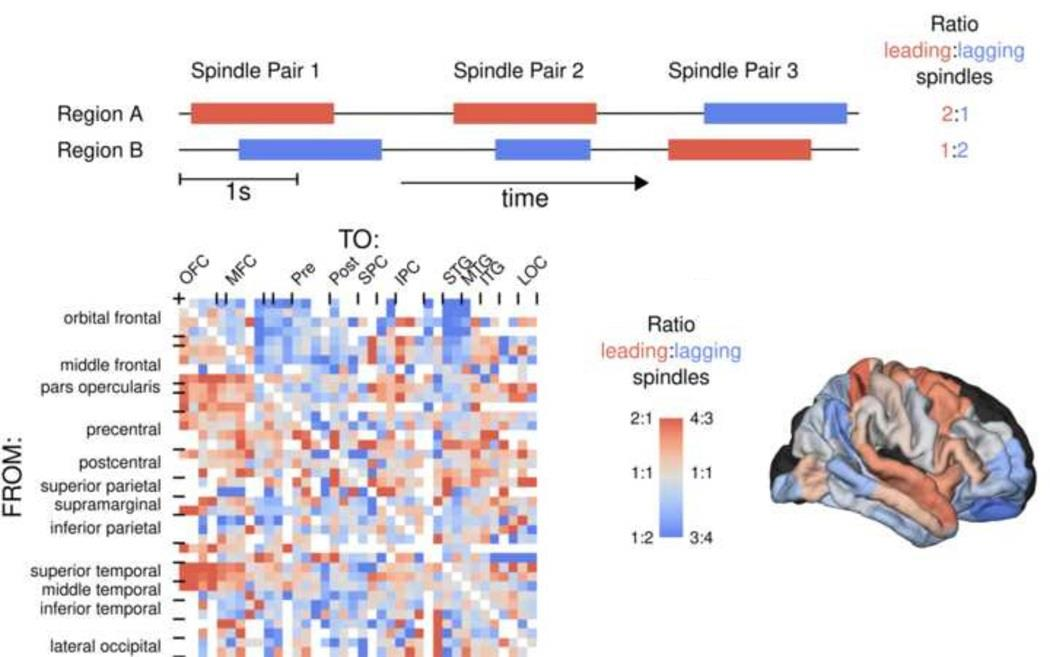
\includegraphics[width=0.8\linewidth]{fig2.25.png}
		\caption{ Spindles tend to propagate from the superior frontal and temporal regions toward the orbitofrontal cortex. Top: Each pair of regions A and B was assigned a ratio based on whether spindles in region A were leading or lagging relative to spindles in region B, resulting in a ratio of 2:1. Bottom left: This measurement was calculated for each pair of regions to generate an antisymmetric matrix representing the directional ratio of spindles between brain regions. We found that spindles in the superior frontal and temporal regions tended to occur before those in the orbitofrontal cortex, with ratios greater than 2:1. Bottom right: The ratio of leading to lagging spindles was averaged for each brain region, indicating regions with a greater tendency to exhibit leading spindles and regions with a greater tendency to exhibit lagging spindles.\cite{Piantoni2017}}
		\label{fig:Directional propagation of sleep spindles}
	\end{figure}
	\begin{figure}[H]
		\centering
		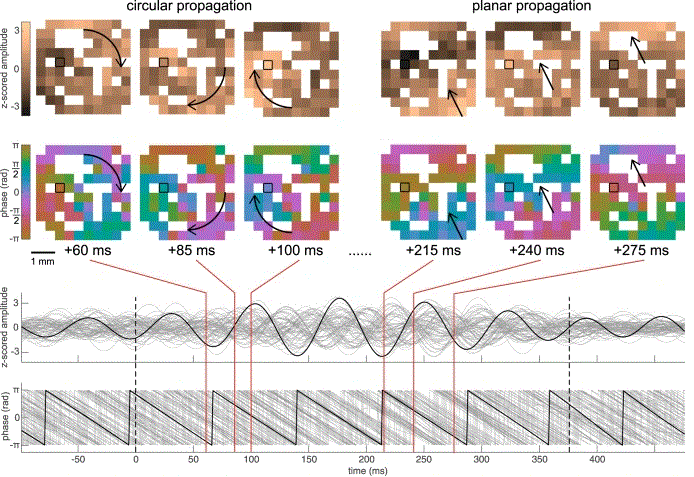
\includegraphics[width=0.8\linewidth]{fig2.26.png}
		\caption{Spindles propagate at a subcentimeter spatial scale. Top left: Circular propagation of a spindle wave shown in three frames of its instantaneous normalized amplitude (z-score) and instantaneous phase. A cyclic colormap was used to represent phase. Top right: Linear propagation of a different wave within the same spindle. White areas indicate bad channels. The channel highlighted in black corresponds to the channel in which the spindle was detected. Arrows indicate the approximate direction of propagation. Bottom: Normalized amplitude and phase. The black waveform and phase correspond to the channel in which the spindle was detected, whereas the gray waveform and phase represent the remaining channels\cite{Dickey2021}}
		\label{fig:Sub-centimeter spindle propagation}
	\end{figure}
	\begin{figure}[H]
		\centering
		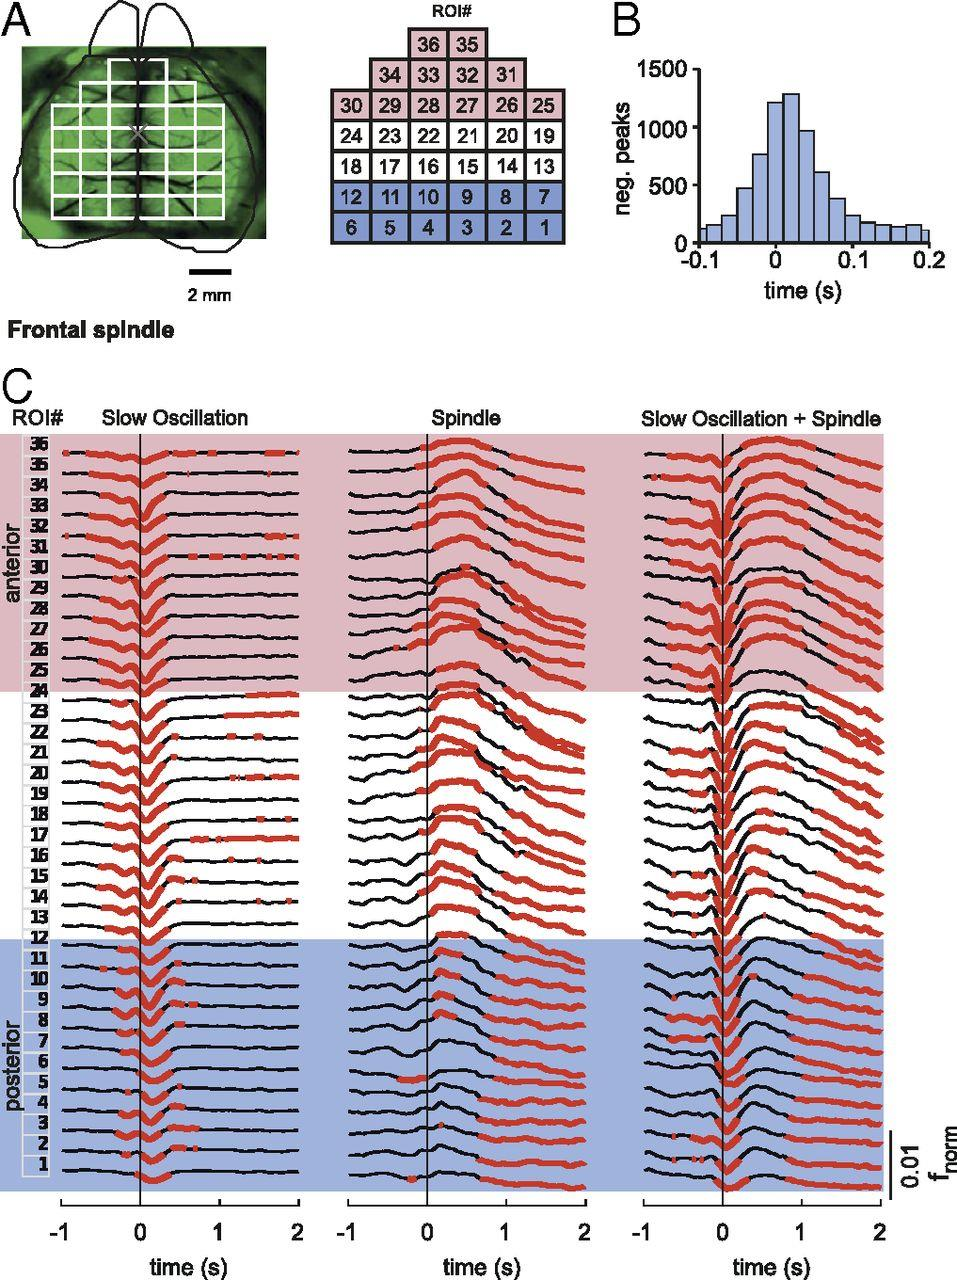
\includegraphics[width=0.8\linewidth]{fig2.27.png}
		\caption{Slow oscillation-related signals propagate from the frontal to the posterior cortex. (A) Illustration of the 36 cortical regions of interest (ROIs) used for imaging. The red area indicates the frontal ROIs (25–36), whereas the blue-shaded area indicates the posterior ROIs (1–12). (B) Histogram showing the distribution of the time delays between the peaks of the negative half-waves of the slow oscillations defined in the signals between the frontal and occipital ROIs. (C) Activity across the 36 ROIs during slow oscillations (left), spindles (middle), and slow oscillations co-occurring with spindles (right; slow oscillation + spindle). The mean raw signal across four animals is shown (n = 706, n = 9,472, and n = 770 for slow oscillations, spindles, and slow oscillations co-occurring with spindles, respectively). Red dots indicate intervals of significantly increased or decreased activity\cite{Niethard2018}}
		\label{fig:Frontal-to-posterior SO propagation}
	\end{figure}
	
	\chapter{Materials and Methods}
	\label{ch:Materials and Methods}
	\section{Introduction}
	\label{sec:Introduction3}
	The present study requires data recorded from the thalamic region. For this purpose, we used the dataset available from the \href{https://buzsakilab.com/wp/datasets}{Buzsáki Lab}, which is associated with Professor Buzsáki's laboratory. The data used in this study consist of simultaneous recordings from the hippocampus and thalamus of mice. The characteristics of these data are described in greater detail in the following sections.
	\section{Data}
	\label{sec:Data}
	As mentioned above, the data consist of simultaneous recordings from the hippocampus and the anterodorsal (AD) nucleus of the mouse thalamus. Therefore, these recordings provide access to thalamic and cortical sleep spindles, slow oscillations in the thalamus and cortex, and ripples and sharp-wave ripples (SPW-Rs) in the hippocampus. The details of the dataset are as follows:
	
	Simultaneous thalamic–hippocampal recordings were obtained from four mice over 18 days, resulting in a total of 18 recording sessions.
	
	It should be noted that spike data are available for both datasets. The raw data were amplified 1,000-fold and recorded at a sampling rate of 20 kHz using a Datamax system with 16-bit resolution. The final sampling rate was 1,250 Hz\cite{Alizadeh2022}.
	\subsection{Recording Electrodes}
	\label{Recording Electrodes}
	The data used by Buzsáki and colleagues were recorded using a 64-channel electrode array in the thalamic region and a five-channel electrode for recordings from the hippocampal region. A brief description of these recording electrodes is provided below\cite{Alizadeh2022}.
	\subsubsection{Buzsáki 64}
	\label{Buzsáki 64}
	This chip is similar to the Buzsáki 32 in terms of its overall appearance and thickness. However, it contains 8 recording electrodes, each of which has 8 channels. The distance between two adjacent electrodes is 200 μm, similar to the Buzsáki 32. The thickness of each electrode is at most 52 μm, and the length of each channel is 5 mm. The total length of the electrode array is 1400 μm (Figure~\ref{fig:Buzsáki 64 chip}).
	\begin{figure}[H]
		\centering
		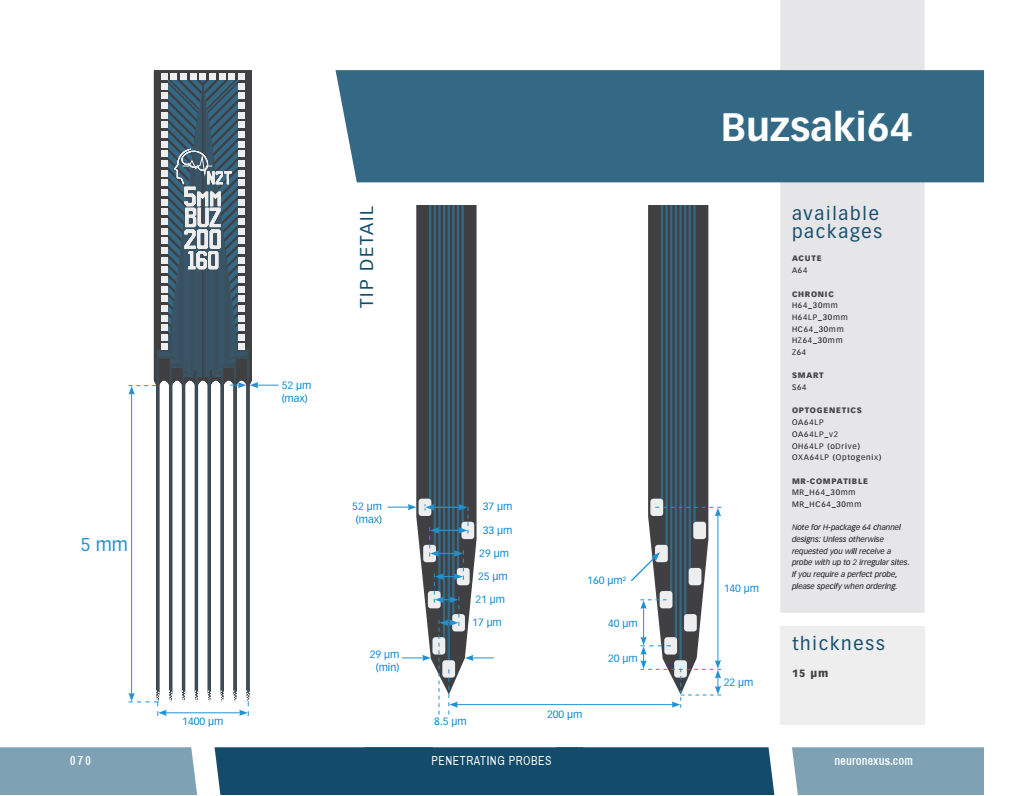
\includegraphics[width=0.8\linewidth]{fig3.1.png}
		\caption{Buzsáki 64 chip\cite{Watson2016}}
		\label{fig:Buzsáki 64 chip}
	\end{figure}
	\section{Data Processing}
	\label{Data Processing}
	\subsection{Data Preprocessing}
	\label{Data Preprocessing}
	Before starting the analysis, it is necessary to ensure that the data are clean. The description of this dataset states that channels containing corrupted signals have already been removed. Therefore, to assess the quality of the recorded signals, we examined the power spectrum of each channel.
	
	To evaluate signal quality based on the power spectrum, we first plotted the power spectrum. The resulting spectrum should exhibit a (1/f) slope\cite{Fernandez2020}. In addition, the presence of a peak at specific frequencies, such as between 8 and 16 Hz, indicates the presence of a sleep spindle in that channel\cite{Fernandez2020}.
	The software used in this study was MATLAB 2022a.
	\subsection{Detection of Slow Oscillations}
	\label{Detection of Slow Oscillations}
	To detect slow oscillations, we used the method described in\cite{Watson2016}. In brief, this method is as follows:
	
	Slow oscillations occur within the frequency range of 0.5–4 Hz. Therefore, the LFP signal was first passed through a band-pass filter with a frequency range of 0.5–4 Hz. Next, the standard deviation of the signal was calculated, and upper and lower thresholds were defined based on this measure. The z-score of the signal was then calculated, and the up and down states were identified based on the z-scored signal and the thresholds determined in the previous step.
	
	It is also known that slow oscillations typically occur within a time window of 500–2000 ms. Therefore, any event that met the above criteria was considered a slow oscillation.
	\subsection{Detection of Sleep Spindles}
	\label{Detection of Sleep Spindles}
	To detect sleep spindles, we used the methods described in\cite{Bernyi2014} and\cite{Watson2016}. In brief, the method is as follows:
	
	Since slow spindles occur in the frequency range of 7–10 Hz and fast spindles in the range of 11–15 Hz, the LFP signal was first filtered within these two frequency ranges. Next, the standard deviation of the signal was calculated, and a threshold was defined. To obtain the signal envelope, the Hilbert transform was applied to the signal within a 0.3-s time window, as the magnitude of the Hilbert transform corresponds to the signal envelope. An event was considered a spindle if the amplitude of its envelope exceeded the defined threshold.
	
	Finally, a temporal criterion was applied to the detected spindles: each spindle had to have a duration between 0.4 and 3.5 s. Events that satisfied both criteria were considered sleep spindles.
	\subsection{Detection of Sharp-Wave Ripples}
	\label{Detection of Sharp-Wave Ripples}
	To detect sharp-wave ripples (SPW-Rs), we used the method described in\cite{Peyrache2011}, which is briefly outlined below.
	
	As mentioned in the Introduction, sharp-wave ripples occur within the frequency range of 150–200 Hz. Therefore, the LFP signal was first filtered within this frequency range. Next, the root mean square (RMS) of the signal was calculated using moving windows. Finally, similar to the detection of sleep spindles and slow oscillations, the standard deviation was used to determine the threshold. The threshold was defined based on the calculated standard deviation.
	
	The z-score of the signal was then calculated by subtracting the mean of the signal from the obtained RMS and dividing the result by the standard deviation. Finally, events whose envelope exceeded the defined threshold were considered sharp-wave ripples.
	\section{Data Analyses}
	\label{Data Analyses}
	\subsection{Time–Frequency Analysis}
	\label{Time–Frequency Analysis}
	For this analysis, we followed the method described in\cite{Bernhard2022}. The FieldTrip toolbox was used to perform wavelet convolution for each event. In this method, frequency steps of 0.25 Hz were used together with a Hanning window with a length corresponding to 5 cycles in time.
	
	Each sleep event was analyzed within its corresponding frequency range. For sleep spindles, the frequency range was set to 5--20 Hz, whereas for sharp-wave ripples, a frequency range of 5--300 Hz was used. The time–frequency matrix was then calculated and normalized. The pre-event time window used for normalization was $-2.5$ to $-1.5$ s for sleep spindles and $-1.5$ to $-1$ s for sharp-wave ripples.
	
	\subsection{Analysis of Phase-locking between Events and Neuronal Activity}
	\label{Analysis of Phase-locking between Events and Neuronal Activity}
	For this analysis, we used the method described in\cite{Dickey2021}. Briefly, after detecting sleep spindles and slow oscillations, these events were divided into two groups: coupled and uncoupled events. A sleep spindle was considered coupled to a slow oscillation if it occurred within 1000 ms of either the up state or down state.
	
	The effect of each coupled event on neuronal activity was then examined separately for each recorded unit using distribution histograms.
	
	\subsection{Separation of Global and Local Sleep Spindles}
	\label{Separation of Global and Local Sleep Spindles}
	To separate sleep spindles into global and local groups, we followed a method similar to that described in\cite{Nir2011}. Briefly, sleep spindles were first detected across all 64 channels of each shank using the method described above. The occurrence times of spindle events were then averaged across all channels.
	
	Next, the distribution of spindle occurrence times was plotted for all recording sessions, and the threshold for separating global and local spindles was determined based on the mean of the medians of these distributions.
	
	Therefore, if a spindle was detected in a number of channels greater than the defined threshold, it was classified as a global spindle; otherwise, it was classified as a local spindle.
	\subsection{Separation of single--peak and double--peak Slow Oscillations} 
	\label{Separation of Bimodal and Unimodal Slow Oscillations}
	To separate single--peak and double--peak slow oscillations, slow oscillations were first detected using the method described above. We then calculated the ratio of the two peaks located within 0.25 s around the main peak. Finally, events for which this ratio was greater than 0.5 were classified as bimodal, whereas the remaining events were classified as unimodal.
	
	\subsection{PAC Analysis between Sleep Spindles and Slow Oscillations} 
	\label{PAC Analysis between Sleep Spindles and Slow Oscillations}
	Phase–amplitude coupling (PAC) analysis was performed as described in\cite{Ladenbauer2017}.
	
	For each event, the phase of the low-frequency oscillation and the phase of the high-frequency oscillation were determined using the Hilbert transform. To ensure accurate estimation of the phase difference, both types of oscillations were filtered within the frequency range of the low-frequency oscillation.
	
	The phase of the low-frequency oscillation was then subtracted from the phase of the high-frequency oscillation.
	
	The phase-locking strength was calculated using the following equation:
	
	$$
	SI = \frac{1}{n}\sum_{t=1}^{n} e^{i(\varphi_l(t)-\varphi_u(t))}
	$$
	
	\subsection{PAC Analysis between Ripples and Sleep Spindles} 
	\label{PAC Analysis between Ripples and Sleep Spindles}
	For this analysis, the same procedure described in \ref{PAC Analysis between Sleep Spindles and Slow Oscillations} was followed, with the difference that the low-frequency events were sleep spindles and the high-frequency events were ripples.
	
	\subsection{Phase Analysis of Sleep Oscillations and Thalamic Neurons} 
	\label{Phase Analysis of Sleep Oscillations and Thalamic Neurons}
	For this analysis, the signal was first filtered within the frequency range of interest. Next, a one-second segment before and after the peak of the oscillatory event of interest was extracted from the signal. The phase of this signal segment was then calculated using the Hilbert transform. Finally, only the phases corresponding to time points at which a spike occurred were extracted from the remaining phases\cite{Alizadeh2022}.
	\subsection{Modulation Index Analysis}
	\label{Modulation Index Analysis}
	To calculate the modulation index, we used a method similar to that described by Yang and colleagues\cite{Watson2016}. This index was used to quantify the relationship between hippocampal neuronal activity and sleep spindles.
	
	To calculate the modulation index, we first obtained a histogram of spike occurrences within a 2-s window before and after the peak of the sleep spindle event. The signal was then smoothed using a 3-s Gaussian window with a width parameter of 6 ms.
	
	Next, surrogate data were generated by shuffling the spike data 100 times using 4-s windows. The mean of the shuffled signal was also calculated within 4-s windows. A histogram of the surrogate spike occurrences around the sleep spindle peak was then obtained.
	
	Finally, the difference between the smoothed signal and the surrogate signal was divided by the 4-s mean values. The modulation index was calculated within a 0.5-s window before and after the sleep spindle peak using this value.
	
	\subsection{Analysis of Sleep Spindle Propagation} 
	\label{Analysis of Sleep Spindle Propagation}
	For this analysis, we used a method similar to that described by Luczak and colleagues\cite{Luczak2007}. First, for each shank of each electrode, we calculated the mean onset time of all detected sleep spindles. We then calculated the mean onset-time delay of spindles in the other shanks relative to the reference shank. Based on the resulting delays, the shanks were ordered according to the direction of spindle propagation.
	\section{Statistical Analyses}
	\label{Statistical Analyses} 
	\subsection{Circular Statistical Tests}
	\label{Circular Statistical Tests} 
	
	In this study, all circular statistical tests were performed using the Circular Statistics Toolbox for MATLAB. In general, the input data for all functions are angular measurements expressed in radians. The following test was used in this study:
	
	\begin{itemize}
		\item Rayleigh test: This test is used to assess whether the distribution of a circular dataset is uniform or non-uniform.
	\end{itemize}
	
	\subsection{Statistical Tests}
	\label{Statistical Tests} 
	To select the appropriate statistical tests, the two datasets were first assessed for normality. If both datasets followed a normal distribution, a t--test was used. If, in addition to being normally distributed, the two datasets had equal sample sizes, an independent-samples t--test was used.
	
	If the two datasets did not follow a normal distribution, non-parametric tests were used. In this case, if the two datasets had equal sample sizes, the rank-sum test was used; otherwise, the paired test was used.
	
	\section{Hypotheses}
	\label{Hypotheses}
	\begin{itemize}
		\item Sleep spindles occur in both local and global forms.
		\item Slow oscillations can occur as either unimodal or bimodal events.
		\item Global spindles are capable of propagating across different brain regions.
		\item Phase-locking between sleep spindles and unimodal and bimodal slow oscillations reflects inter-network connectivity and memory consolidation.
		\item The behavior of sleep events differs between global and local states.
		\item Few studies have investigated spindles separately in the thalamic regions and their relationship with the hippocampus.
		\item Neuronal activity in the AD region of the thalamus during characteristic NREM sleep events in mice can be investigated.
		\item The characteristics of unimodal slow oscillations differ from those of bimodal slow oscillations.
	\end{itemize}
	\section{Problem Statement}
	\label{Problem Statement}
	Living organisms spend a considerable portion of their lifetime asleep. Therefore, understanding sleep and the events that occur in the brain during sleep is highly important.
	
	Over the years, many researchers have investigated brain activity during sleep, including characteristic sleep events such as slow oscillations, sleep spindles, and SPW-Rs. Numerous studies have confirmed the role of characteristic sleep oscillations in memory consolidation. On the other hand, recent studies conducted in the cortex have shown that the propagation of these oscillations has a direct effect on memory consolidation and learning. Similarly, phase-locking between sleep spindles and slow oscillations reflects inter-network connectivity as well as memory consolidation. The behavior of these events also differs depending on whether they are global or local. Since these characteristics have a direct effect on memory function, understanding the behavior of events according to their local or global distribution is of considerable importance. However, most studies conducted in humans and animals have focused primarily on the cortical regions of the brain, and relatively few studies have investigated these events in the thalamus and hippocampus.
	
	The novelty of the present study lies in investigating characteristic sleep oscillations in the AD region of the thalamus, specifically sleep spindles and slow oscillations, by classifying sleep spindles into global and local groups and slow oscillations into unimodal and bimodal groups. In addition, the characteristics of these events, including their duration and amplitude, will be investigated and compared. Furthermore, the relationship between unimodal and bimodal slow oscillations in the thalamus and sleep spindles will be examined. To investigate the connectivity between the thalamus and hippocampus, the relationship between global and local thalamic spindles and hippocampal ripples will also be examined.
	
	Finally, given the important role of thalamic sleep spindles in memory consolidation, their propagation patterns will also be investigated.
	
	%%%%%%%%%%%%%%%%%%%%%%%%%%%%%%%%%%%%%%%
	\chapter{Results}
	\label{ch:Results}
	\section{Separation of Sleep Spindles and Slow Oscillations}
	\label{Separation of Sleep Spindles and Slow Oscillations}
	\subsection{Global and Local Sleep Spindles}
	\label{Global and Local Sleep Spindles}
	Global and local sleep spindles were separated using the method described above. An example of global and local sleep spindles is shown in Figure~\ref{fig:Example of global and local spindles}.
	The percentages of global and local sleep spindles for the 18 recording sessions are presented in Appendix \ref{tab:global_local_spindles}.
	
	By examining the percentages of global and local sleep spindles across the 18 recording sessions and using a t-test, it was found that thalamic spindles were significantly more likely to be local (Figure\ref{fig:spindle hist}).
	
	Next, the characteristics of sleep spindles were compared between these two groups. When comparing the peak amplitudes of spindles in the two groups, a significant difference in peak amplitude was observed across all recording sessions. In addition, a positive correlation was found between the peak amplitudes of global and local spindles.
	
	Regarding the duration of local and global spindles, a significant difference between their mean durations was observed in 72\% of the recording sessions. A positive correlation was also found between the durations of global and local spindles (Figure\ref{fig:fig4.3}).
	\begin{figure}[!htbp]
		\centering
		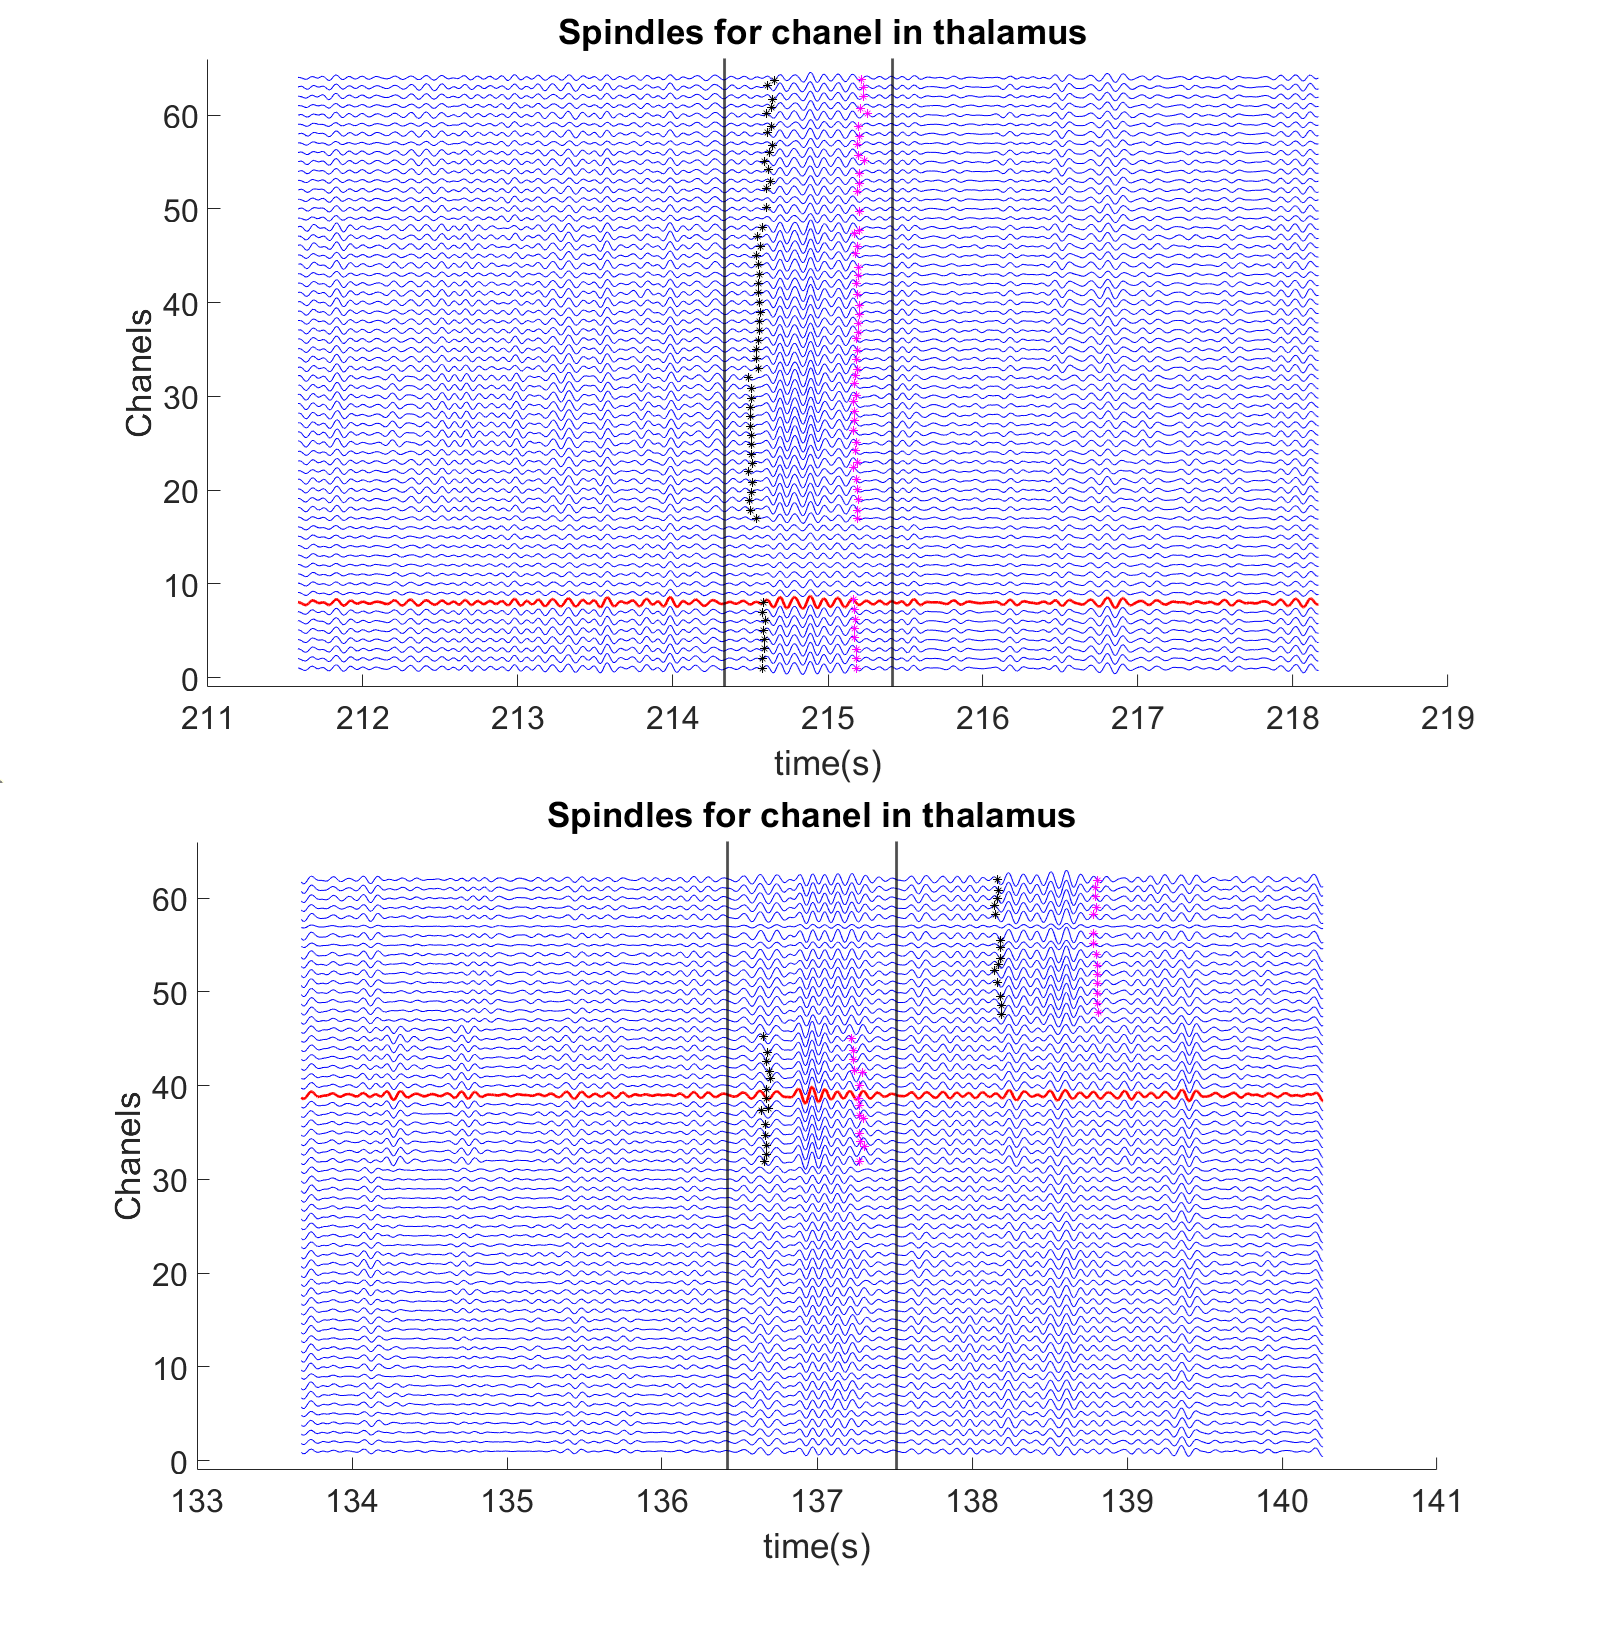
\includegraphics[width=0.8\linewidth]{fig4.1.png}
		\caption{Example of global and local spindles. (Top) A global spindle; (bottom) a local spindle. The red channel represents the reference channel. The black marker indicates the spindle onset, and the pink marker denotes the spindle offset}
		\label{fig:Example of global and local spindles}
	\end{figure}

	\begin{figure}[!htbp]
		\centering
		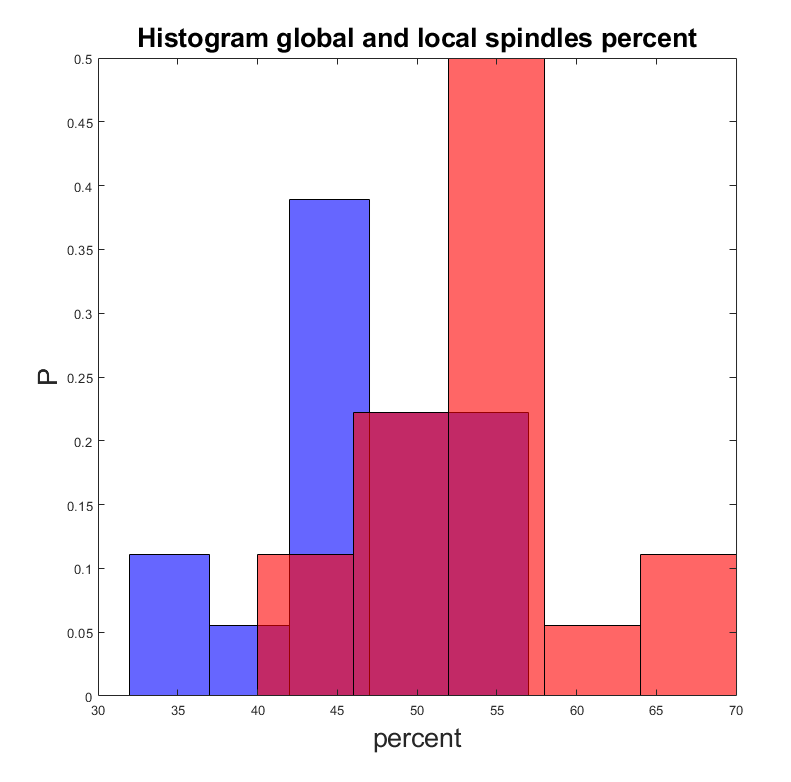
\includegraphics[width=0.8\linewidth]{fig4.2.png}
		\caption{The histogram of global (blue) and local (red) spindle percentages shows that thalamic spindles exhibit a significant tendency to be local}
		\label{fig:spindle hist}
	\end{figure}
	
	\begin{figure}[!htbp]
		\centering
		
		% TOP ROW
		\begin{minipage}{0.48\textwidth}
			\raggedright
			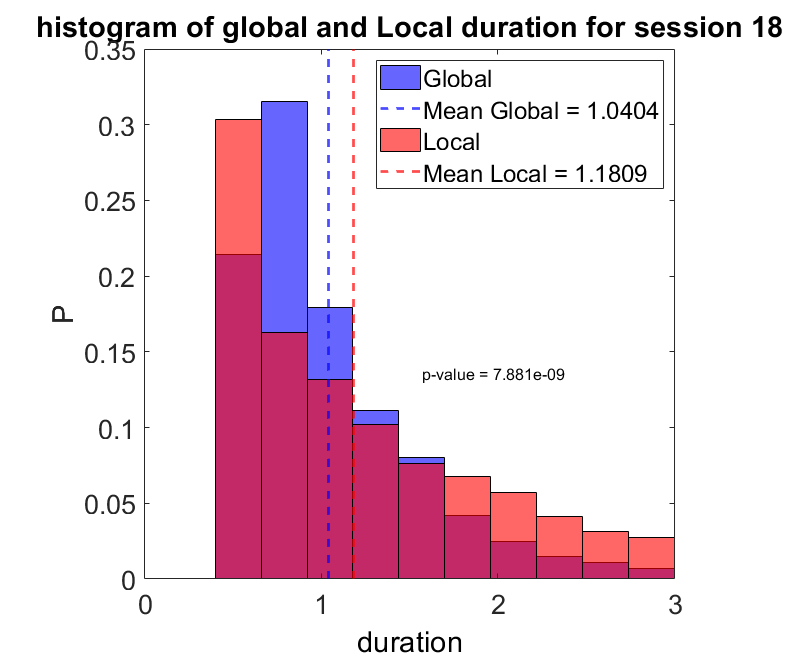
\includegraphics[width=0.95\textwidth]{fig4.3 top right .png}
		\end{minipage}
		\hfill
		\begin{minipage}{0.48\textwidth}
			\raggedleft
			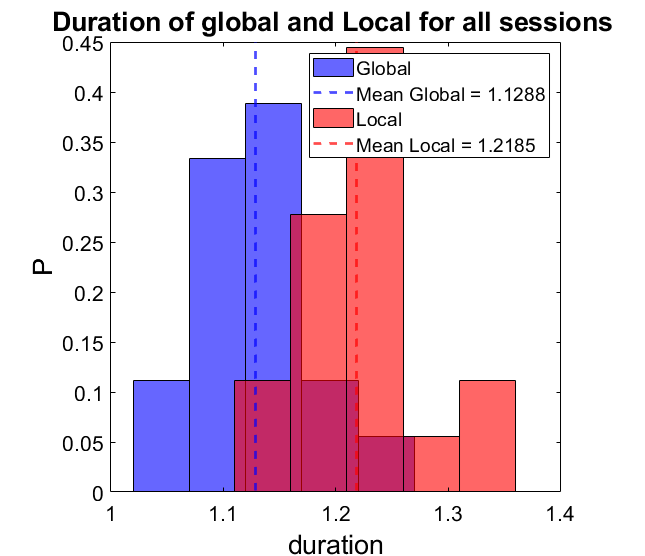
\includegraphics[width=0.95\textwidth]{fig4.3 top left.png}
		\end{minipage}
		
		\vspace{0.5cm}
		
		% CENTER IMAGE
		\begin{minipage}{0.7\textwidth}
			\centering
			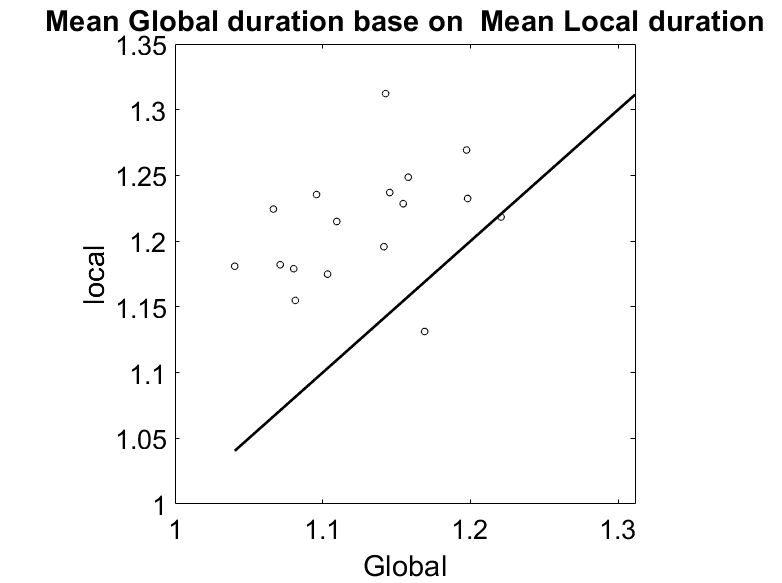
\includegraphics[width=\textwidth]{fig4.3 center.png}
		\end{minipage}
		
		\caption{Comparison of the duration of global and local spindles. Top-left: comparison for a single session. Top-right: comparison across all sessions. Bottom: statistical significance.}
		\label{fig:fig4.3}
	\end{figure}
		
	
	%\FloatBarrier
	\section{Separation of Single-Peak and Double-Peak Slow Oscillations}
	\label{Separation of Single-Peak and Double-Peak Slow Oscillations}
	To separate slow oscillations into single-peak and double-peak groups, after detecting the slow oscillations, the ratio between the two peaks within a 0.25-s time window around the main peak was calculated, and its distribution was plotted as a histogram. Based on the histograms obtained for all 18 recording sessions, a ratio of 0.5 was selected as the threshold (Figure~\ref{fig:fig4.4}).
	
	\begin{figure}[htbp]
		\centering
		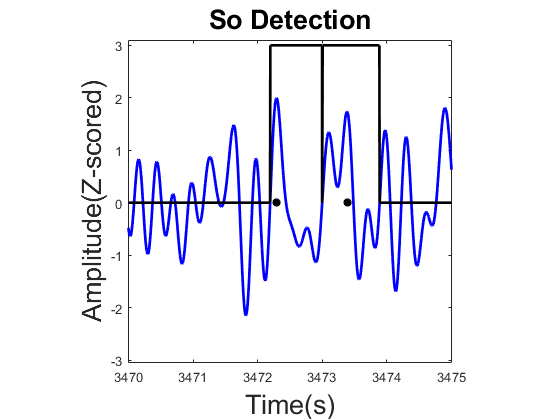
\includegraphics[width=0.5\linewidth]{fig4.4.png}
		\caption{An example of single-peak and double-peak slow oscillations}
		\label{fig:fig4.4}
	\end{figure}
	The numbers of single-peak and double-peak slow oscillations, together with their total number and the percentage of each type of event, are presented in Appendix~\ref{tab:single_double_slow_oscillations}
	
	Next, by comparing the percentages of single-peak and double-peak slow oscillations across all recording sessions, it was found that there was no significant difference between the two groups across any of the recording sessions.
	Similar to the comparisons performed for sleep spindles, the characteristics of single-peak and double-peak slow oscillations were also compared.
	
	First, the amplitudes of single-peak and double-peak slow oscillations were compared. A significant difference in amplitude was observed in 100\% of the recording sessions (Figure~\ref{fig:fig4.5}).
	
	Comparison of the durations of single-peak and double-peak slow oscillations showed that, overall, there was no significant difference between the two groups. A session-by-session analysis also showed that no significant difference was present in 83\% of the recording sessions (Figure~\ref{fig:fig4.6}).
	
	\section{Analysis of Neuronal Activity Around Spindle Events and Slow Oscillations}
	\label{Analysis of Neuronal Activity Around Spindle Events and Slow Oscillations}
	\subsection{Neuronal Activity Around Global and Local Sleep Spindles}
	\label{Neuronal Activity Around Global and Local Sleep Spindles}
	Analysis of the modulation index (MI) within the time window extending 0.25 s before and after the spindle peak showed that, among 465 neurons across the 18 recording sessions, neuronal activity was phase-locked to spindle peaks. In 61\% of the neurons, this phase-locking was stronger during global spindles than during local spindles. Comparison of this difference across all neurons showed a significant difference between the two spindle groups (Figure~\ref{fig:fig4.8} and Figure~\ref{fig:fig4.7}).
	
\begin{figure}[!htbp]
	\centering
	
	% TOP ROW
	\begin{minipage}{0.48\textwidth}
		\raggedright
		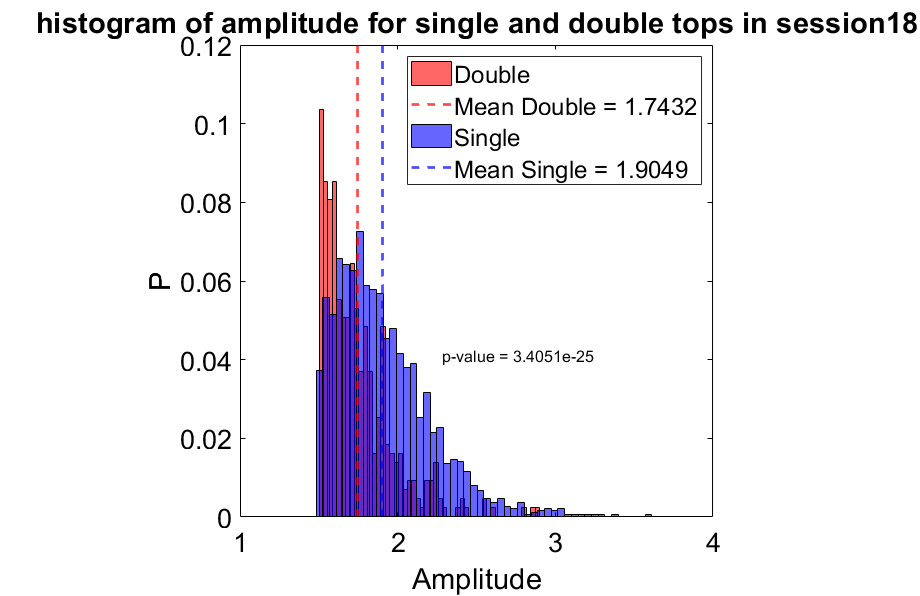
\includegraphics[width=1\textwidth]{fig4.5 top right.png}
	\end{minipage}
	\hfill
	\begin{minipage}{0.48\textwidth}
		\raggedleft
		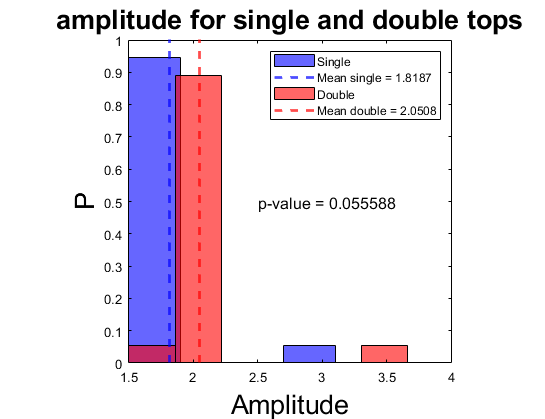
\includegraphics[width=1.2\textwidth]{fig4.5 top left.png}
	\end{minipage}
	
	\vspace{0.5cm}
	
	% CENTER IMAGE
	\begin{minipage}{0.7\textwidth}
		\centering
		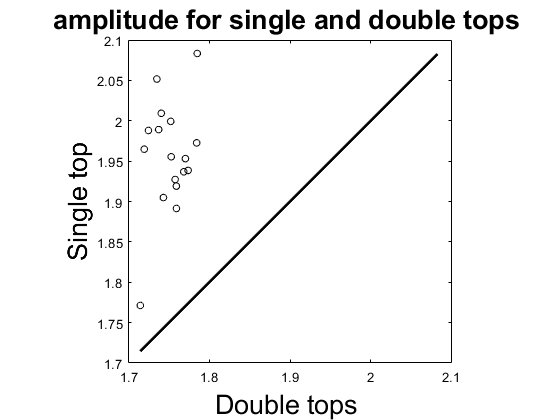
\includegraphics[width=\textwidth]{fig4.5 center.png}
	\end{minipage}
	
	\caption{Comparison of the amplitude of single-peak and double-peak slow oscillations. Top-left: comparison for a single session. Top-right: comparison across all sessions. Bottom: statistical significance.}
	\label{fig:fig4.5}
\end{figure}

\begin{figure}[!htbp]
	\centering
	
	\begin{minipage}{0.48\textwidth}
		\centering
		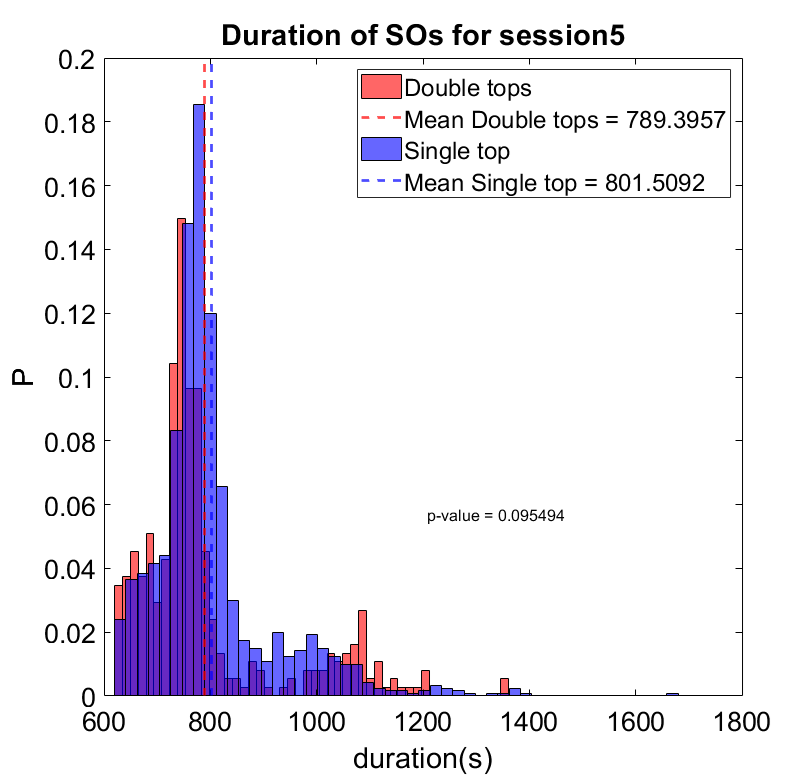
\includegraphics[width=\textwidth]{fig4.6 left.png}
	\end{minipage}
	\hfill
	\begin{minipage}{0.48\textwidth}
		\centering
		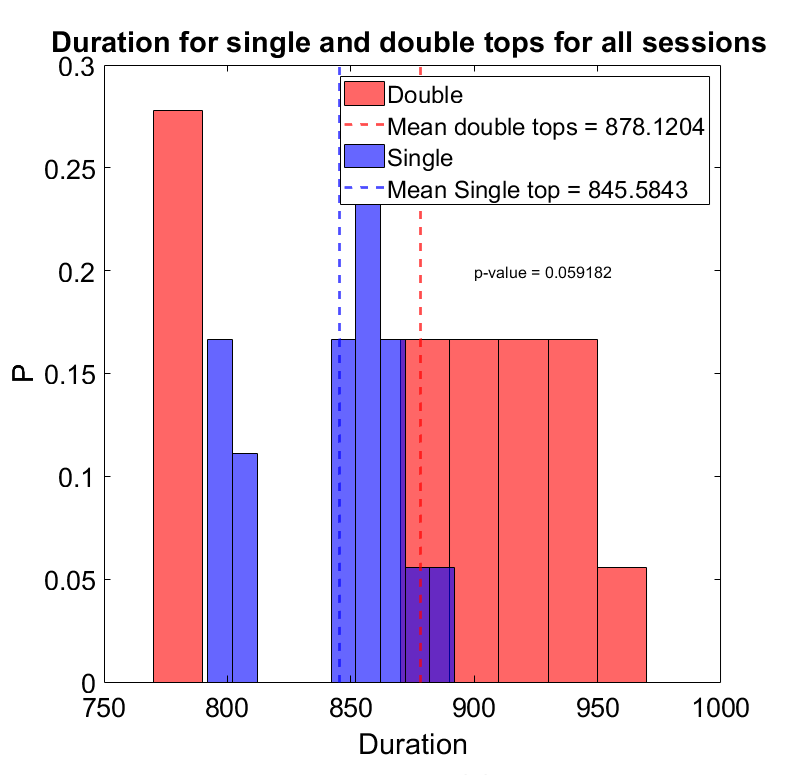
\includegraphics[width=\textwidth]{fig4.6 right.png}
	\end{minipage}
	
	\caption{Comparison of the duration of single-peak and double-peak slow oscillations. left: comparison for a single session. right: comparison across all sessions}
	\label{fig:fig4.6}
\end{figure}

\begin{figure}[!htbp]
	\centering
	
	\begin{minipage}{0.48\textwidth}
		\centering
		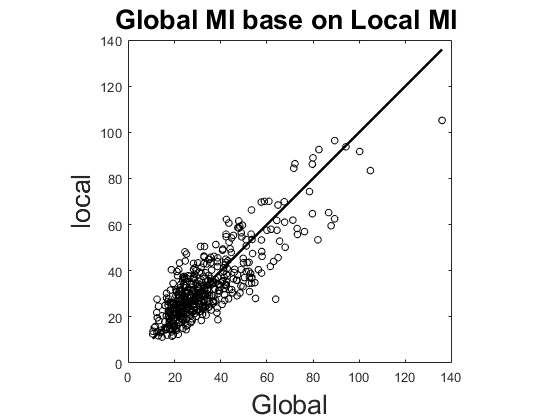
\includegraphics[width=\textwidth]{fig4.7 left.png}
	\end{minipage}
	\hfill
	\begin{minipage}{0.48\textwidth}
		\centering
		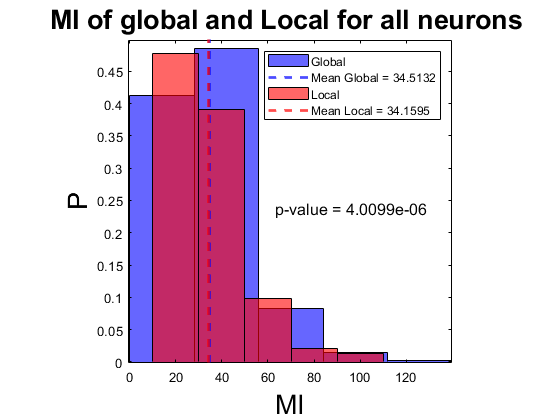
\includegraphics[width=\textwidth]{fig4.7 right.png}
	\end{minipage}
	
	\caption{Right: Neuronal activity around sleep spindles for all neurons. Left: MI values for each neuron, separated for local and global spindles.}
	\label{fig:fig4.7}
\end{figure}

\begin{figure}[!htbp]
	\centering
	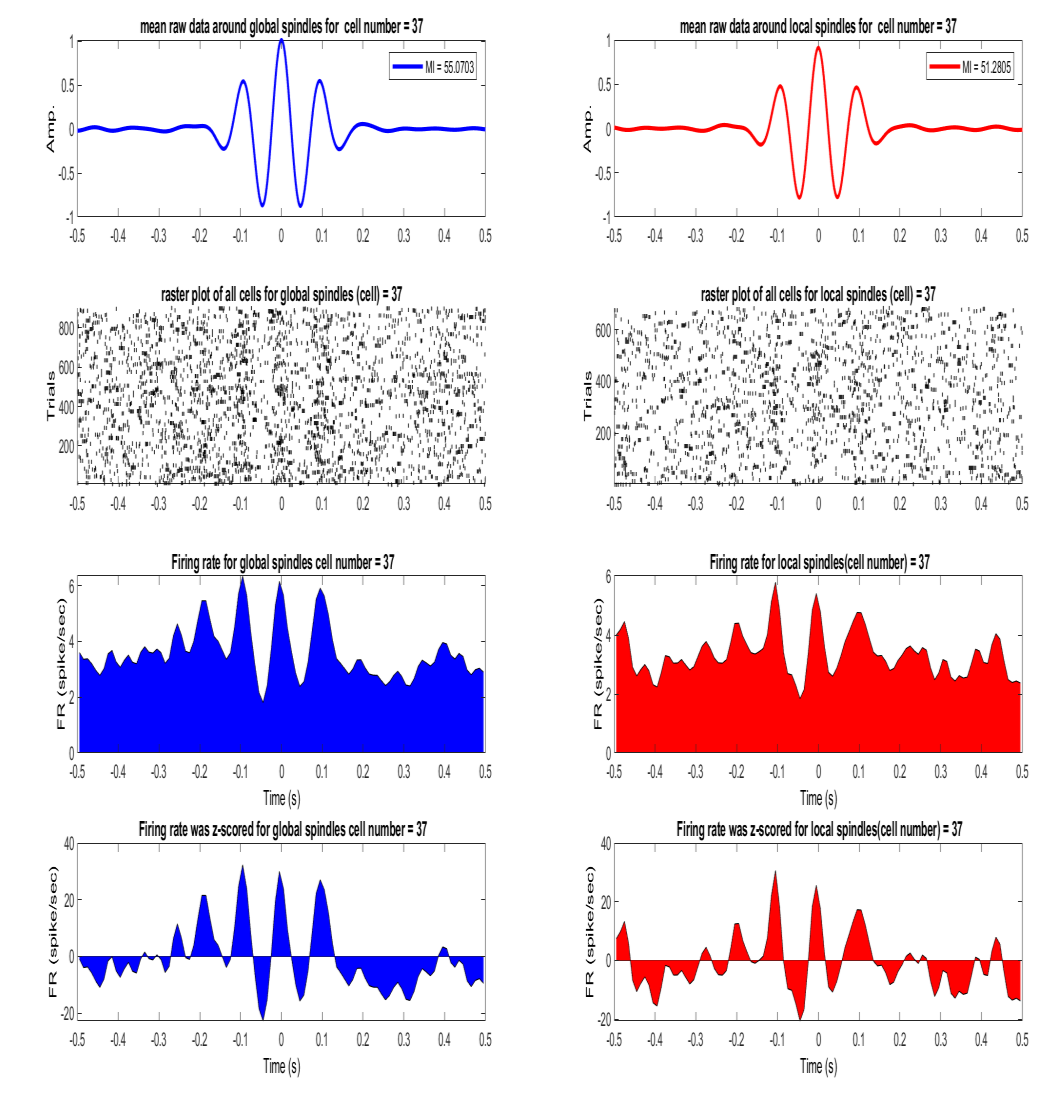
\includegraphics[width=1\linewidth]{fig4.8.png}
	\caption{ Neuronal activity around spindles for a single neuron. Row 1: Mean activity for global and local spindles. Row 2: Raster plot of the neuron around global and local spindles. Row 3: Neuronal activity around global and local spindles. Row 4: Normalized neuronal activity around global and local spindles}
	\label{fig:fig4.8}
\end{figure}

\subsection{Neuronal Activity Around Single-Peak and Double-Peak Slow Oscillations}
\label{Neuronal Activity Around Single-Peak and Double-Peak Slow Oscillations}
For 465 neurons across 18 recording sessions, the modulation index (MI) was examined within a 0.25s window around the main peak of the slow oscillation. In 83\% of the neurons, neuronal activity was greater during single-peak slow oscillations than during double-peak slow oscillations. Statistical analysis across all neurons further showed that the higher MI observed for single-peak slow oscillations was statistically significant (Figure~\ref{fig:fig3.9} and Figure~\ref{fig:fig4.10}).
\begin{figure}
	\centering
	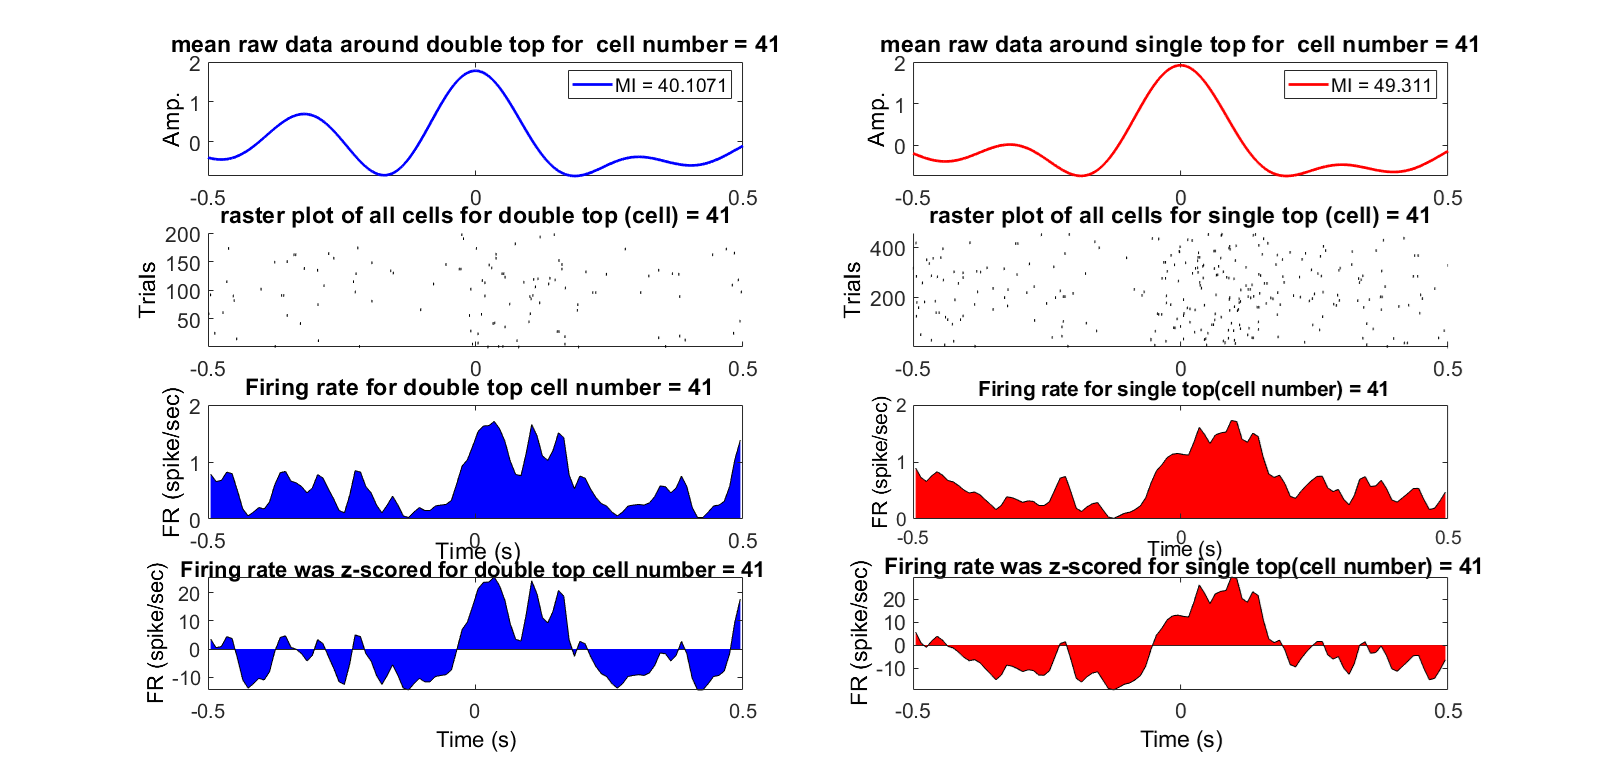
\includegraphics[width=1\linewidth]{fig3.9.png}
	\caption{Neuronal activity around slow oscillations for a single neuron. Row 1: Mean single-peak and double-peak slow oscillations. Row 2: Raster plot of the neuron around single-peak and double-peak slow oscillations. Row 3: Neuronal activity around single-peak and double-peak slow oscillations. Row 4: Normalized neuronal activity around single-peak and double-peak slow oscillations.}
	\label{fig:fig3.9}
\end{figure}

\begin{figure}[!htbp]
	\centering
	
	\begin{minipage}{0.48\textwidth}
		\centering
		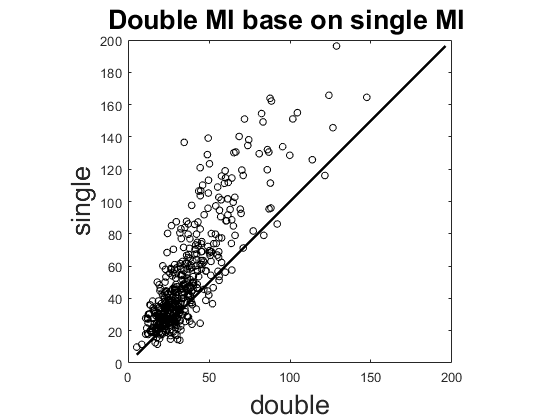
\includegraphics[width=\textwidth]{fig4.10 left.png}
	\end{minipage}
	\hfill
	\begin{minipage}{0.48\textwidth}
		\centering
		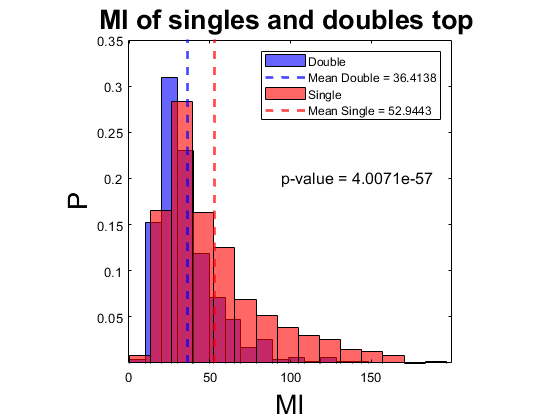
\includegraphics[width=\textwidth]{fig4.10 right.png}
	\end{minipage}
	
	\caption{Right: Neuronal activity around sleep slow oscillations for all neurons. Left: MI values for each neuron, separated for single-peak and double-peak slow oscillations.}
	\label{fig:fig4.10}
\end{figure}

\section{Relationship Between Single-Peak and Double-Peak Slow Oscillations and Sleep Spindles}
\label{Relationship Between Single-Peak and Double-Peak Slow Oscillations and Sleep Spindles}
Using the phase–amplitude coupling (PAC) method described in the Methods section, we investigated the relationship between sleep spindles and the two types of detected slow oscillations.
Using this method, it was found that the phases of both groups of slow oscillations were phase-locked to sleep spindles; however, no significant difference in their strength was observed (Figure~\ref{fig:fig4.11} and Figure~\ref{fig:fig4.12}).
\begin{figure}
	\centering
	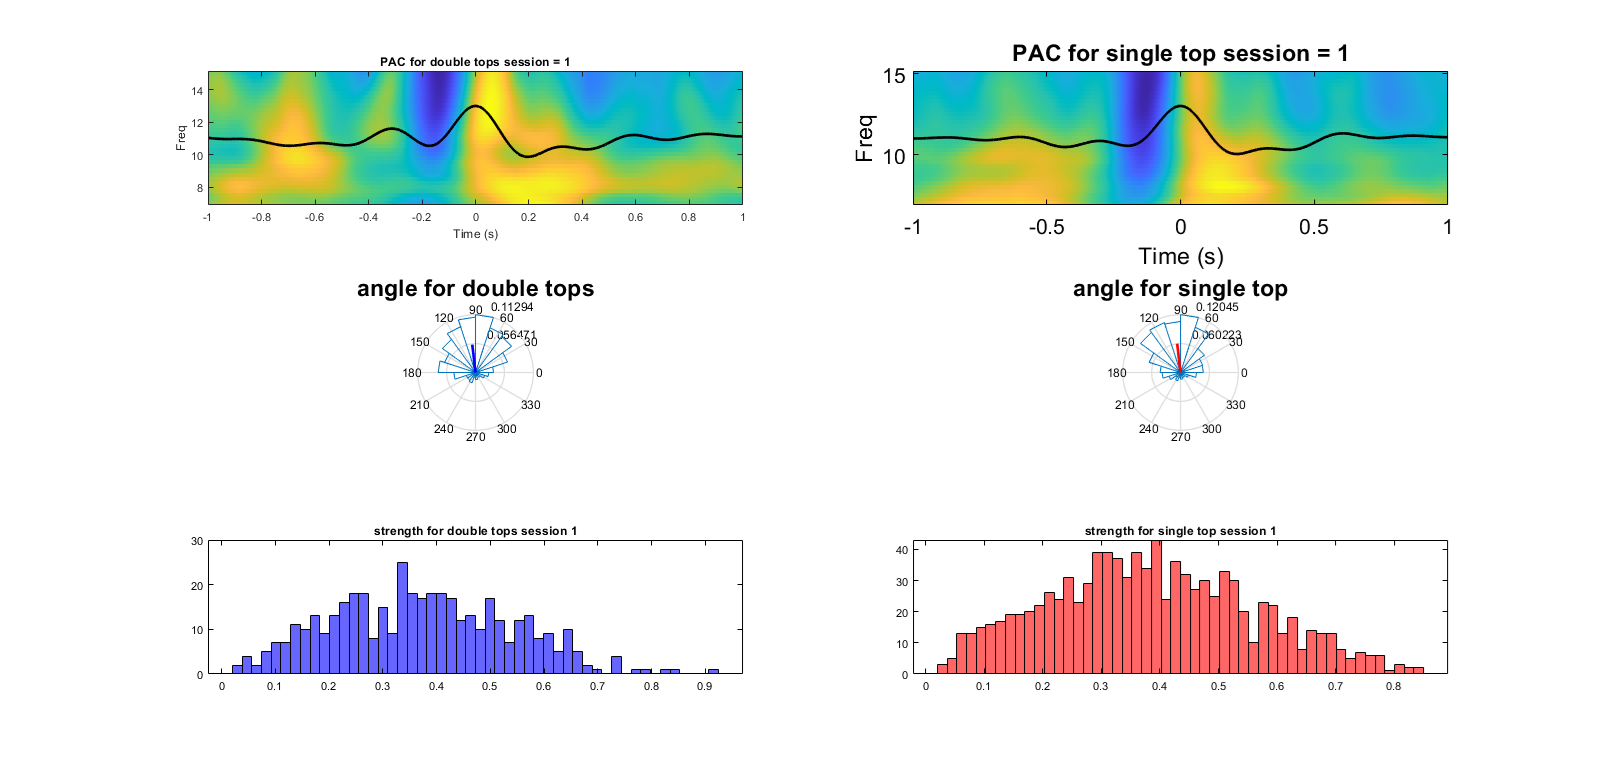
\includegraphics[width=1\linewidth]{fig4.11.png}
	\caption{PAC analysis between single-peak and double-peak slow oscillations and spindles in a single session. Row 1:Time-frequency characteristics between slow oscillations and spindles. Row 2: Phase. Row 3: PAC magnitude.}
	\label{fig:fig4.11}
\end{figure}

\begin{figure}[!htbp]
	\centering
	
	% TOP ROW
	\begin{minipage}{0.48\textwidth}
		\raggedright
		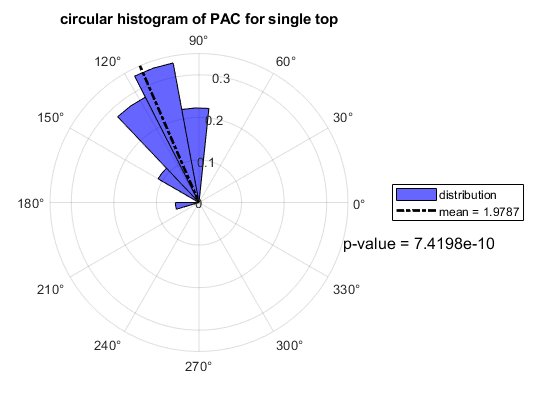
\includegraphics[width=1\textwidth]{fig4.12 right top.png}
	\end{minipage}
	\hfill
	\begin{minipage}{0.48\textwidth}
		\raggedleft
		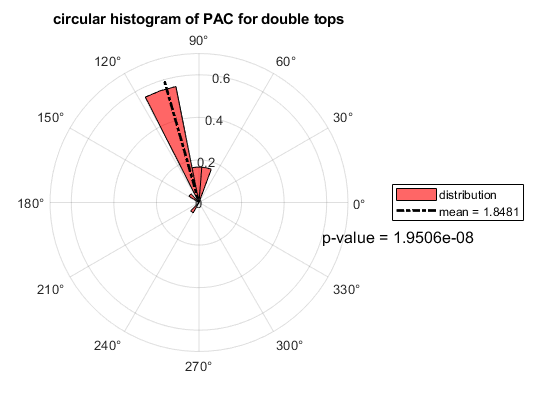
\includegraphics[width=1.2\textwidth]{fig4.12 left top.png}
	\end{minipage}
	
	\vspace{0.5cm}
	
	% CENTER IMAGE
	\begin{minipage}{0.7\textwidth}
		\centering
		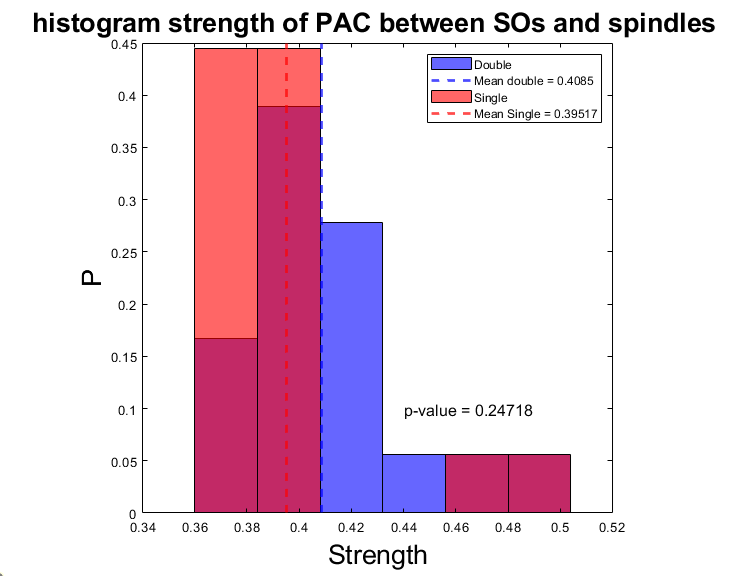
\includegraphics[width=\textwidth]{fig4.12 center.png}
	\end{minipage}
	
	\caption{PAC analysis across all sessions. Top-left: PAC phase for single-peak slow oscillations. Top-right: PAC phase for double-peak slow oscillations. Bottom: PAC strength for single-peak and double-peak slow oscillations.}
	\label{fig:fig4.12}
\end{figure}

\section{Propagation of Spindles}
\label{Propagation of Spindles}
Following the method described in the Methods section, we first calculated the sorted median time delay separately for each recording session. We then determined the delay of each individual spindle detected in the reference channel and calculated its correlation with the sorted median delay. To investigate whether this difference in delay was consistently observed across all spindles in the reference channel, we plotted the corresponding histogram for each recording session. It was observed that, in most recording sessions, the fourth electrode was the primary site of spindle onset. In addition, the median correlation of the delays was positive across all recording sessions, indicating the presence of spindle propagation (Figure~\ref{fig:fig3.13}).
\begin{figure}[!htbp]
	\centering
	
	% TOP ROW
	\begin{minipage}{0.48\textwidth}
		\raggedright
		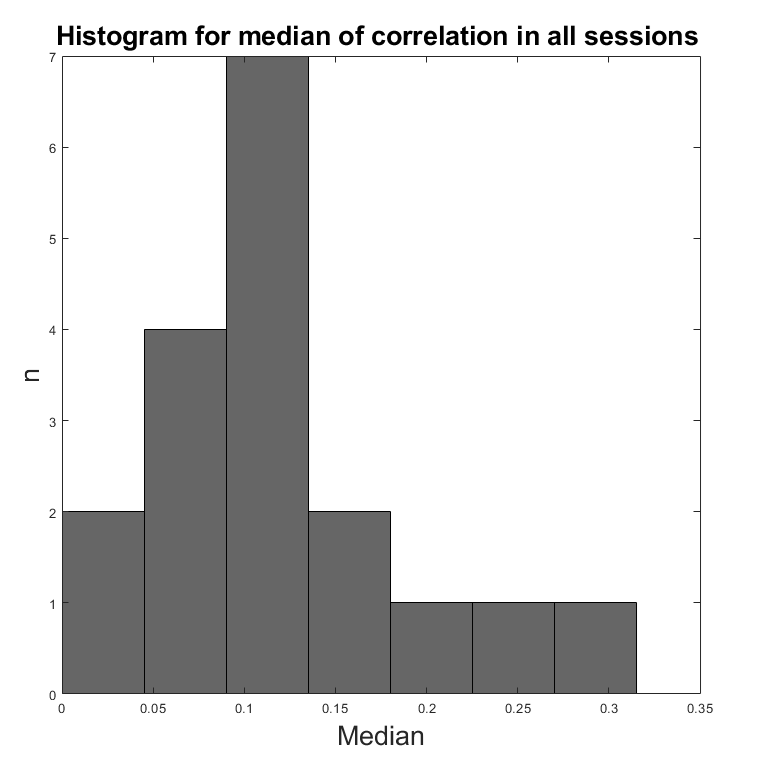
\includegraphics[width=1\textwidth]{fig3.13 right top.png}
	\end{minipage}
	\hfill
	\begin{minipage}{0.48\textwidth}
		\raggedleft
		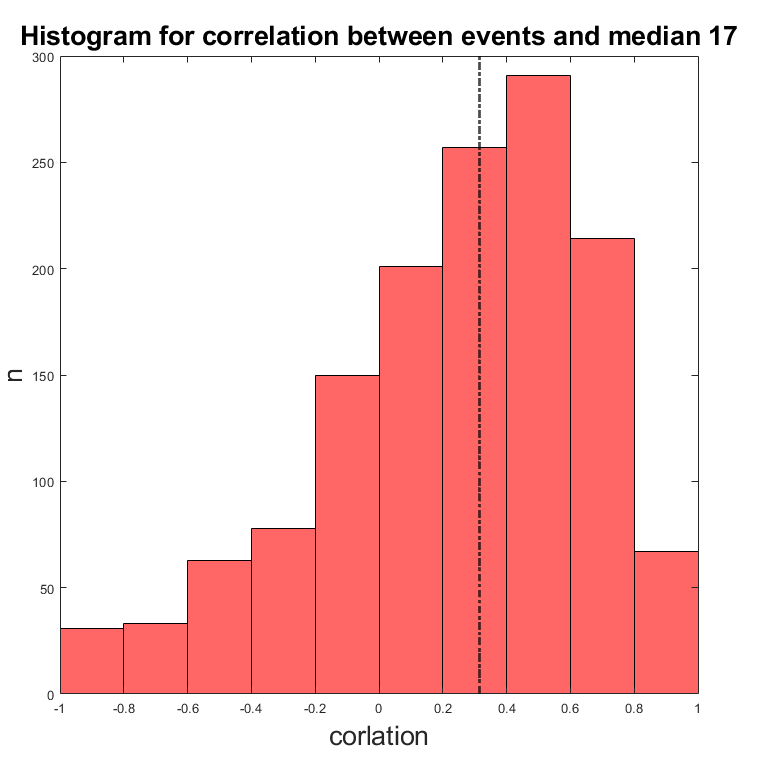
\includegraphics[width=1.2\textwidth]{fig3.13 left top.png}
	\end{minipage}
	
	\vspace{0.5cm}
	
	% CENTER IMAGE
	\begin{minipage}{0.7\textwidth}
		\centering
		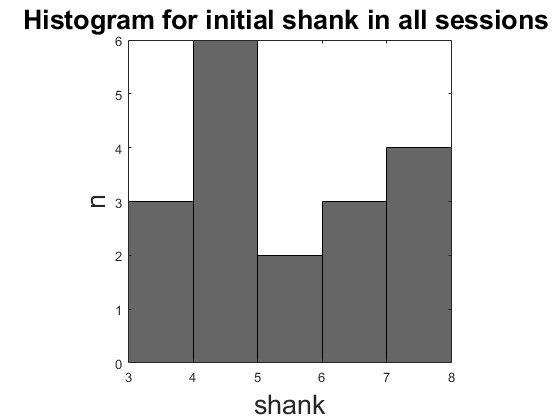
\includegraphics[width=\textwidth]{fig3.13 center.png}
	\end{minipage}
	
	\caption{Top-left: Histogram of median correlation between the delays of reference channel spindles and other channels across all sessions. Top-right: Histogram of correlations between the delays of spindles in different channels relative to the reference channel for a single session (dashed line indicates the median). Bottom: Histogram of spindle-initiating channels across all sessions.}
	\label{fig:fig3.13}
\end{figure}

\section{Relationship Between Spindles and Ripples}
\label{Relationship Between Spindles and Ripples}
As mentioned in Chapter~\ref{Introduction}, sleep spindles are events originating from the thalamic region, whereas ripples are events originating from the hippocampal region, and these two types of events also occur at different frequency ranges.

\begin{figure}
	\centering
	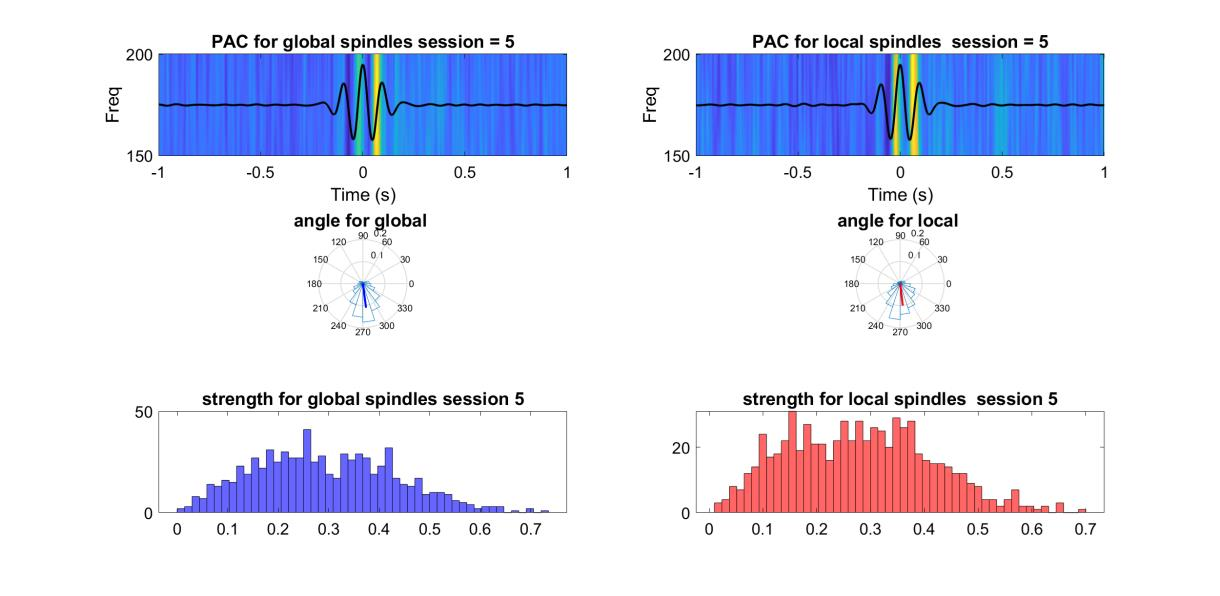
\includegraphics[width=1\linewidth]{fig4.14.png}
	\caption{PAC analysis between global and local spindles in a single session. Row 1: Time-frequency characteristics between spindles and ripples. Row 2: Phase. Row 3: PAC magnitude.}
	\label{fig:fig4.14}
\end{figure}


To compare these two similar events, we used the PAC analysis described in Section~\ref{Relationship Between Single-Peak and Double-Peak Slow Oscillations and Sleep Spindles}. The analysis showed that the phases of both global and local spindles were phase-locked to ripples; however, no significant difference was observed in the strength of this phase-locking (Figure~\ref{fig:fig4.14} and Figure~\ref{fig:fig4.15}).

\begin{figure}[!htbp]
	\centering
	
	% TOP ROW
	\begin{minipage}{0.48\textwidth}
		\raggedright
		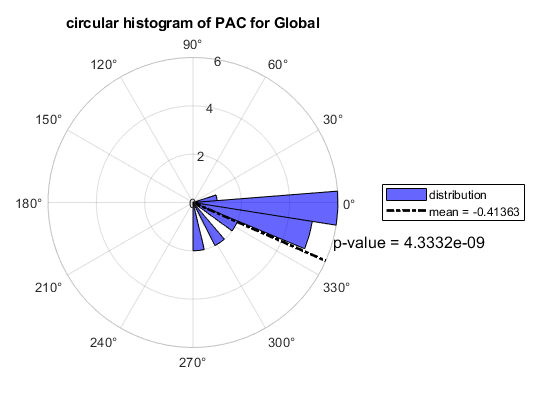
\includegraphics[width=1\textwidth]{fig4.15 top left.png}
	\end{minipage}
	\hfill
	\begin{minipage}{0.48\textwidth}
		\raggedleft
		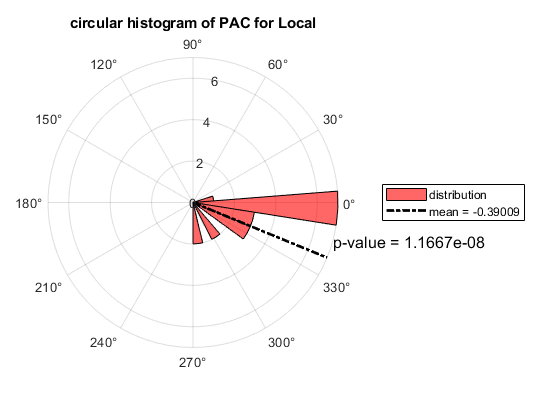
\includegraphics[width=1.2\textwidth]{fig4.15 top right.png}
	\end{minipage}
	
	\vspace{0.5cm}
	
	% CENTER IMAGE
	\begin{minipage}{0.7\textwidth}
		\centering
		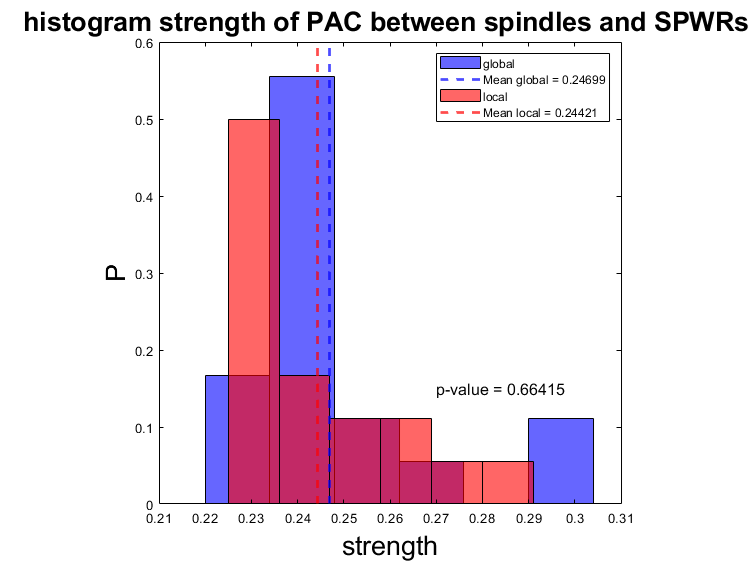
\includegraphics[width=\textwidth]{fig4.15 center.png}
	\end{minipage}
	
	\caption{PAC analysis across all recording sessions. Top right: PAC phase for global and local spindles. Top left: PAC phase for global and local spindles. Bottom: PAC strength for global and local spindles.
	}
	\label{fig:fig4.15}
\end{figure}

\chapter{Discussion and Conclusion}
\label{Discussion and Conclusion}


In this study, global and local sleep spindles were separated using the methods described above. The results presented in the figures and tables indicate significant differences between local and global spindles. In particular, statistical analysis using the t-test showed that thalamic spindles were significantly more likely to be local.

Compared with previous studies, these findings may indicate fundamental differences in the functional mechanisms underlying sleep spindles. Previous studies have mainly focused on global spindles and have shown that these spindles are involved in cognitive processes such as memory and learning. However, the findings of the present study suggest that local spindles may have distinct roles that have received less attention in previous research.

Significant differences were also observed in the peak amplitude and duration of spindles between the two groups. These differences may reflect variations in the neuronal mechanisms responsible for spindle generation. In addition, the positive correlations observed between the peak amplitudes of global and local spindles, as well as between their durations, may indicate complex relationships between these two types of spindles.

Overall, these findings may contribute to a better understanding of sleep physiology and the role of sleep spindles in this process. Further research in this area may help identify new approaches for the treatment of sleep disorders and for improving quality of life. Such studies may also provide a better understanding of the role of sleep in health and daily functioning.

In this study, slow oscillations were divided into two groups: single-peak and double-peak slow oscillations. Using histogram analysis, a peak ratio of 0.5 was selected as the threshold for separating the two groups. This threshold provided a basis for distinguishing between single-peak and double-peak slow oscillations. These results, together with the data presented in Appendix~\ref{tab:single_double_slow_oscillations}, allow a more detailed comparison between the two types of slow oscillations.

Based on the comparison of the percentage of slow oscillation events, no significant difference was observed between the two groups across the recording sessions. These findings suggest that, overall, single-peak and double-peak slow oscillations may follow similar mechanisms.

When comparing the amplitudes of the two types of slow oscillations, a significant difference was observed in a considerable proportion of the recording sessions. This may indicate differences in neuronal activity or experimental conditions across individual recording sessions. However, regarding the duration of the slow oscillations, no significant difference was observed between the two groups in most recording sessions. This finding may indicate a degree of temporal consistency in slow oscillations under different conditions.

These findings can be compared with previous studies that have focused on slow oscillations and their effects on cognitive processes and brain function. Previous research has shown that slow oscillations may play an important role in regulating cognitive states and coordinating neuronal activity across the brain. Further investigation in this area may provide a better understanding of the role of slow oscillations in brain processes and their relationship with other neurophysiological phenomena. Such information may contribute to the development of new approaches for the diagnosis and treatment of neurological disorders.

The findings of the present study indicate that neuronal activity was phase-locked to spindle peaks, particularly during global spindles. These findings further support the importance of interactions between neuronal activity and sleep spindles in the study of sleep neurophysiology. The following discussion provides a more detailed interpretation of these findings and compares them with previous studies.

In the present study, neuronal activity was examined in 465 neurons across 18 recording sessions. Neuronal activity was phase-locked to spindle peaks, and in 61\% of the neurons, this phase-locking was stronger during global spindles than during local spindles. These results indicate a strong relationship between neuronal activity and global spindles and may suggest an important role for global spindles in coordinating neuronal activity across different brain regions.

Comparison with previous studies indicates that, although earlier research has focused on the relationship between sleep spindles and neuronal activity, the specific role of global spindles has received relatively less attention. Studies investigating local spindles have suggested that these events may be involved in local processes such as attention and sensory processing. In contrast, the present findings suggest that global spindles may be more strongly involved in processes that require broader coordination across the brain, such as memory and learning.

The findings of this study support the possibility that global spindles play an important role in coordinating neuronal activity across the brain. These results may contribute to a better understanding of the role of sleep spindles in cognitive processes and brain function. They may also provide a basis for developing new approaches for the diagnosis and treatment of sleep disorders and for improving quality of life. Further research in this area may provide additional insight into the role of sleep spindles in health and daily functioning.

The findings of this study also indicate substantial differences in neuronal activity associated with single-peak and double-peak slow oscillations. These differences may be related to variations in the neuronal mechanisms underlying the generation of these oscillations. Single-peak slow oscillations may be associated with specific cognitive processes that require greater neuronal activity.

Compared with previous studies, these findings may contribute to a better understanding of the role of slow oscillations in cognitive processes and brain function. Previous studies have primarily focused on the relationship between slow oscillations and neuronal activity, whereas the distinction between single-peak and double-peak slow oscillations has received relatively less attention.

The findings of the present study highlight the importance of differences between single-peak and double-peak slow oscillations in neuronal activity. These differences may provide further insight into the neuronal mechanisms underlying slow oscillation generation and their role in cognitive processes. They may also contribute to the development of new approaches for the diagnosis and treatment of neurological disorders and for improving quality of life. Further research in this area may provide a better understanding of the role of slow oscillations in health and daily functioning.

In this study, phase–amplitude coupling (PAC) analysis was used to investigate the relationship between sleep spindles and the two types of slow oscillations. The results showed that the phases of slow oscillations were phase-locked to sleep spindles; however, no significant difference was observed in the strength of this coupling between the two groups. These findings are consistent with previous studies investigating the relationship between the phase of brain oscillations and sleep-related neuronal activity.

Previous studies have investigated the relationship between slow brain oscillations and different stages of sleep. For example, Mölle et al. (2002)\cite reported that slow oscillations during deep sleep were phase-locked to neural activity associated with memory processes. Similarly, Studer et al. (2014) showed that slow oscillations may be associated with different cognitive processes, including attention and memory.

However, the findings of the present study indicate that although phase-locking exists between slow oscillations and sleep spindles, this relationship is not necessarily accompanied by an increase in coupling strength. One possible explanation is that sleep spindles and slow oscillations may operate at different levels of neural processing, such that their interaction is primarily related to temporal and phase relationships rather than to coupling strength.

To better understand these relationships and their differences, future studies should investigate the underlying mechanisms of phase-locking in greater detail and examine its effects on cognitive processes and memory. In addition, the use of more advanced imaging techniques and more detailed statistical analyses may help identify more complex patterns of interaction between slow oscillations and sleep-related activity. Such investigations may contribute to the development of new therapeutic approaches for sleep disorders and the improvement of cognitive function.

In this study, spindle time delays were analyzed across different recording sessions. First, using the method described above, the median time delay was calculated separately for each recording session. Subsequently, the delay of each individual spindle detected in the reference channel was determined, and its correlation with the sorted median delay was calculated. To examine the consistency of this delay difference across all spindles detected in the reference channel, the corresponding histograms were plotted for each recording session.

The results showed that, in most recording sessions, the fourth electrode acted as the primary site of spindle onset, and the median correlation of the delays was positive across all recording sessions, indicating the presence of spindle propagation. These findings are consistent with previous studies emphasizing spindle propagation as an important phenomenon in neural processes.
\begin{itemize}
	\item Stability of the delay difference: The histograms showed that the delay difference was relatively consistent across the detected spindles, which may indicate a specific neural pattern underlying spindle propagation.
	
	\item Role of the fourth electrode: The fourth electrode was identified as the primary site of spindle onset. This finding may contribute to a better understanding of the neural mechanisms underlying spindle generation and propagation.
	
	\item Positive correlation: The positive median correlation of the delays across all recording sessions further supports the presence of spindle propagation and is consistent with previous findings in this area.
	
\end{itemize}
Stability of the delay difference: The histograms showed that the delay difference was relatively consistent across the detected spindles, which may indicate a specific neural pattern underlying spindle propagation.

Role of the fourth electrode: The fourth electrode was identified as the primary site of spindle onset. This finding may contribute to a better understanding of the neural mechanisms underlying spindle generation and propagation.

Positive correlation: The positive median correlation of the delays across all recording sessions further supports the presence of spindle propagation and is consistent with previous findings in this area.

Overall, this analysis and its findings may contribute to a better understanding of the neural mechanisms underlying sleep spindles and may provide a basis for future studies investigating spindle propagation and its functional significance.

Using PAC analysis, sleep spindles originating from the thalamic region were compared with ripples originating from the hippocampal region. These two phenomena occur at different frequency ranges and are both considered important in neural and cognitive processes.

The PAC analysis showed that the phases of sleep spindles and ripples were phase-locked; however, no significant difference was observed in the strength of this coupling. These findings may suggest that although both phenomena are involved in related neural processes, their precise mechanisms of interaction may differ.

Previous studies have emphasized the roles of both sleep spindles and ripples in memory and learning. For example, Siapas and Wilson (1998) showed that hippocampal ripples may be associated with synaptic potentiation and memory consolidation. Sleep spindles, on the other hand, have also been associated with the regulation of neuronal activity and the coordination of brain activity during sleep.

The present findings suggest that phase-locking between sleep spindles and ripples may be more closely related to the frequency and timing of neuronal activity than to the strength of the coupling. This observation may provide further insight into how these two types of neural activity interact and how their interaction may contribute to cognitive processes.

To further clarify these relationships, future studies should investigate the underlying mechanisms of this phase-locking in greater detail and examine its effects on memory and learning processes. In addition, investigating the differences between the various frequency components and their interactions with other forms of neural activity may provide a better understanding of these phenomena.

Ultimately, further research in this area may contribute to the development of new therapeutic approaches for sleep- and memory-related disorders and may help improve quality of life. The present study can also provide a basis for future investigations and contribute to advancing knowledge in the field of neuroscience.

In future studies, the relationship between neuronal activity and global and local spindles in the slow and fast frequency ranges could be investigated separately. In addition, the duration and amplitude of separately detected slow and fast spindles, as well as the propagation of global and local spindles across individual shanks, could be examined in greater detail. Furthermore, the relationship between ripples and single-peak and double-peak slow oscillations could be investigated to provide further insight into the interactions between hippocampal and thalamocortical sleep events.


\chapter{Appendix}
\appendix
\label{appendix1}

\begin{table}[H]%[htbp]
	\centering
	\caption{Number of global and local sleep spindles across all recording sessions.}
	\label{tab:global_local_spindles}
	\begin{tabular}{lccc}
		\hline
		\textbf{Mouse Name} & \textbf{Total Spindles} & \textbf{Global Spindles (\%)} & \textbf{Local Spindles (\%)} \\
		\hline
		Mouse12-120806 & 1265 & 56.75 & 43.24 \\
		Mouse12-120807 & 1280 & 57.75 & 42.24 \\
		Mouse12-120808 & 1341 & 52.64 & 47.36 \\
		Mouse12-120809 & 1611 & 49.29 & 50.71 \\
		Mouse12-120810 & 1444 & 52.15 & 47.85 \\
		Mouse17-130128 & 1323 & 46.79 & 53.21 \\
		Mouse17-130129 & 1620 & 43.52 & 56.48 \\
		Mouse17-130131 & 1631 & 39.37 & 60.64 \\
		Mouse17-130201 & 1355 & 47.61 & 52.39 \\
		Mouse17-130202 & 1417 & 45.95 & 54.057 \\
		Mouse17-130203 & 1642 & 47.19 & 52.81 \\
		Mouse17-130204 & 1645 & 45.72 & 54.28 \\
		Mouse20-130514 & 1125 & 32.36 & 67.64 \\
		Mouse20-130515 & 1801 & 34.54 & 65.46 \\
		Mouse20-130516 & 1475 & 43.12 & 56.88 \\
		Mouse20-130517 & 1456 & 43.00 & 57.00 \\
		Mouse20-130520 & 1393 & 48.53 & 51.47 \\
		Mouse32-140822 & 2399 & 42.02 & 57.98 \\
		\hline
	\end{tabular}
\end{table}

\appendix
\label{appendix2}
\begin{table}[H]
	\centering
	\caption{Number of single-peak and double-peak slow oscillations across all recording sessions.}
	\label{tab:single_double_slow_oscillations}
	
	\begin{tabular}{l
			>{\centering\arraybackslash}p{2cm}
			>{\centering\arraybackslash}p{2.5cm}
			>{\centering\arraybackslash}p{2.5cm}
			>{\centering\arraybackslash}p{2cm}
			>{\centering\arraybackslash}p{2cm}}
		\hline
		\textbf{Mouse Name} &
		\textbf{Total Slow Oscillations} &
		\centering\arraybackslash\textbf{Double-Peak Slow Oscillations} &
		\centering\arraybackslash\textbf{Single-Peak Slow Oscillations} &
		\centering\arraybackslash\textbf{Double-Peak (\%)} &
		\centering\arraybackslash\textbf{Single-Peak (\%)} \\
		\hline
		
		Mouse12-120806 & 1476 & 708 & 768 & 47.97 & 52.03 \\
		Mouse12-120807 & 1915 & 671 & 1244 & 35.04 & 64.96 \\
		Mouse12-120808 & 1902 & 667 & 1235 & 35.07 & 64.93 \\
		Mouse12-120809 & 2275 & 780 & 1495 & 34.29 & 65.71 \\
		Mouse12-120810 & 1732 & 560 & 1172 & 32.33 & 67.67 \\
		Mouse17-130128 & 1562 & 399 & 1163 & 25.54 & 74.46 \\
		Mouse17-130129 & 1653 & 444 & 1209 & 26.86 & 73.14 \\
		Mouse17-130131 & 2487 & 742 & 1745 & 29.84 & 70.16 \\
		Mouse17-130201 & 1827 & 423 & 1404 & 23.15 & 76.85 \\
		Mouse17-130202 & 2026 & 521 & 1505 & 25.72 & 74.28 \\
		Mouse17-130203 & 2276 & 575 & 1701 & 25.26 & 74.74 \\
		Mouse17-130204 & 2422 & 593 & 1829 & 24.48 & 75.52 \\
		Mouse20-130514 & 160 & 105 & 55 & 65.63 & 34.38 \\
		Mouse20-130515 & 1967 & 904 & 1063 & 45.96 & 54.04 \\
		Mouse20-130516 & 1749 & 747 & 1002 & 42.71 & 57.29 \\
		Mouse20-130517 & 1486 & 574 & 912 & 38.63 & 61.37 \\
		Mouse20-130520 & 281 & 84 & 197 & 29.89 & 70.11 \\
		Mouse32-140822 & 2926 & 699 & 2227 & 23.89 & 76.11 \\
		
		\hline
	\end{tabular}
\end{table}

\appendix

\begin{table}[H]
	\centering
	\caption{List of abbreviations used in this study.}
	\label{tab:abbreviations}
	
	\begin{tabular}{>{\centering\arraybackslash}p{3cm}
			>{\centering\arraybackslash}p{8cm}}
		\hline
		\textbf{Abbreviation} & \textbf{Full Name} \\
		\hline
		
		NREM & Non-Rapid Eye Movement \\
		SO & Slow Oscillation \\
		SPWR & Sharp-Wave Ripples \\
		REM & Rapid Eye Movement \\
		EEG & Electroencephalography \\
		Hz & Hertz \\
		EOG & Electrooculography \\
		EMG & Electromyography \\
		SWS & Slow-Wave Sleep \\
		LFP & Local Field Potential \\
		MUA & Multi-Unit Activity \\
		DG & Dentate Gyrus \\
		TRN & Thalamic Reticular Nucleus \\
		CM & Centromedial \\
		AD & Anterodorsal \\
		AC & Anterior Cingulate \\
		VB & Ventrobasal Complex of the Thalamus \\
		BC & Barrel Cortex \\
		VC & Visual Cortex \\
		
		\hline
	\end{tabular}
\end{table}

\bibliographystyle{IEEEtran}
\bibliography{References}

%======================
\end{document}
